\documentclass[12pt,a4paper]{article}
\usepackage[utf8]{inputenc}
\usepackage[english]{babel}
\usepackage{amsmath}
\usepackage{amssymb}
\usepackage{amsthm}
\usepackage{graphicx}
\usepackage[hidelinks]{hyperref}
\usepackage{bookmark}
\usepackage{listings}
\usepackage{xcolor}
\usepackage{colortbl}
\usepackage{float}
\usepackage{booktabs}
\usepackage{geometry}
\usepackage[ruled,vlined]{algorithm2e}
\usepackage{tikz}
\usetikzlibrary{shapes,mindmap,trees,positioning}
\usepackage{pgfplots}
\pgfplotsset{compat=1.18}
\usepackage{imakeidx}
\makeindex
\usepackage{tcolorbox}
\usepackage{cancel}
\usepackage{pdflscape}
\usepackage{refcount}
\usepackage[round]{natbib}

% Page margins
\geometry{margin=1in}

% Theorem environments
\theoremstyle{definition}
\newtheorem{definition}{Definition}[section]
\newtheorem{theorem}{Theorem}[section]
\newtheorem{lemma}{Lemma}[section]

% Code listing style
\lstset{
    language=Python,
    basicstyle=\ttfamily\small,
    keywordstyle=\color{blue},
    commentstyle=\color{green!60!black},
    stringstyle=\color{red},
    numbers=left,
    numberstyle=\tiny\color{gray},
    frame=single,
    breaklines=true,
    captionpos=b
}

% Title information
\title{Automatic Reasoning and Planning\\
\large Course Summary - Master's Degree}
\author{Carlos Alberto Botina Carpio\\
Universidad Internacional de la Rioja\\
\href{mailto:carlos.botina621@comunidadunir.net}{carlos.botina621@comunidadunir.net}}
\date{\today}

\begin{document}

\maketitle

\begin{abstract}
This document contains a summary of the Automatic Reasoning and Planning course syllabus for the Master's Degree. It includes a summary of the main topics covered during the sessions, as well as additional explanations and extensions of the concepts and techniques referenced in class. The purpose of this document is to serve as study material and reference for the course contents.

Notice that this document is fully customized to the author's needs, placing greater emphasis on topics that the author struggles with or has not yet mastered, while covering more briefly those topics that are already well understood by the author.

\end{abstract}

\newpage
\tableofcontents
\newpage

% Lecture 001
\section*{Lecture 001}
\section{Introduction to Decision Making}
\label{sec:decision-making}

Decision making is a complex process that requires evaluating and understanding environmental conditions. In many cases, decisions become so intricate that we need to exhaustively evaluate every possible scenario. This is where mathematics becomes useful in helping us make informed decisions.

When making decisions, the following elements are involved:

\begin{itemize}
    \item \textbf{Future effect}: What is the duration of the decision's impact? (short-term, long-term)
    \item \textbf{Reversibility}: Is it easy to reverse the decision?
    \item \textbf{Impact}: How many areas or domains are affected?
    \item \textbf{Quality}: Ethics, legality, behavioral principles, workplace relationships, etc.
    \item \textbf{Periodicity}: How frequently must this decision be made?
\end{itemize}

\subsection{Decision Classification}
\label{subsec:decision-classification}

Decisions can be classified into two main categories: \textbf{high-level} and \textbf{low-level} decisions. High-level decisions are strategic, have long-term consequences, are difficult to reverse, and affect multiple areas of an organization or system. They are typically exceptional and require careful consideration of various quality factors. In contrast, low-level decisions are operational, have minimal future impact, are easily reversible, and affect fewer areas. They are made frequently and have limited impact on important quality factors.

Table~\ref{tab:decision_classification} summarizes the characteristics that distinguish high-level from low-level decisions based on the elements involved in decision making.

\begin{table}[H]
\centering
\caption{Classification of decisions: High-level vs. Low-level}
\label{tab:decision_classification}
\begin{tabular}{p{4.5cm}p{4.5cm}p{4.5cm}}
\toprule
 & \textbf{High Level} & \textbf{Low Level} \\
\midrule
\textbf{Future Effect} & Affect the future & Don't affect the future \\
\midrule
\textbf{Reversibility} & Difficult reversibility & Reversible \\
\midrule
\textbf{Impact} & Broad impact & Little impact \\
\midrule
\textbf{Quality Factors} & Affect many important & Affect few important \\
\midrule
\textbf{Periodicity} & Exceptional & Frequent \\
\bottomrule
\end{tabular}
\end{table}

Decisions can also be classified as \textbf{programmed} or \textbf{non-programmed}. Programmed decisions have a well-defined step-by-step sequence that is known and can be followed. For example, in case of an emergency, one calls the emergency number. Non-programmed decisions are unique and specific to the situation, with no defined rules or steps to follow.

\subsection{Problem Classification}
\label{subsec:problem-classification}

Problems can be classified as \textbf{structured} or \textbf{non-structured}:

\begin{itemize}
    \item \textbf{Structured problems}: The problem contains all the information needed to solve it. All necessary data, constraints, and conditions are available from the start.
    \begin{itemize}
        \item \textit{Example}: Solving a system of linear equations where all coefficients and constants are given.
    \end{itemize}
    
    \item \textbf{Non-structured problems}: The problem does not contain all the information needed to solve it. To solve it, we need to search for additional information.
    \begin{itemize}
        \item \textit{Example}: Diagnosing a medical condition where symptoms are present but additional tests, patient history, or expert consultation are required to reach a diagnosis.
    \end{itemize}
\end{itemize}


\section{Problem Solving Stages}

\subsection{First Stage: Understand the Problem's Complexity}

There are many techniques to understand a problem's complexity, which can be organized into two main categories:

\begin{itemize}
    \item \textbf{Identify the problem}: Self-questioning about the problem (origin, magnitude, focus, or history), SWOT analysis (Strengths, Weaknesses, Opportunities, Threats), discussion meetings (Scrum), etc.
    
    \item \textbf{Explain the problem}: Go beyond the surface and investigate the underlying causes of the problem. This can be done using various techniques such as ERIM problem classification, the 20 causes technique, the Ishikawa diagram (fishbone diagram), and other root cause analysis methods.

\end{itemize}

We must, therefore, create problem definitions that present characteristics that allow us to work with them efficiently. Some characteristics or assumptions that can be made in simple environments (well-defined problems) are:

\begin{itemize}
    \item \textbf{Discrete}: The world can be conceived in states. In each state there is a finite set of perceptions and actions.
    
    \item \textbf{Accessible}: The agent can access the relevant characteristics of the environment. It can determine the \textbf{current state} of the world and the \textbf{state it would like to reach}.
    
    \item \textbf{Static and deterministic}: There is no temporal pressure nor uncertainty. The world changes only when the agent acts. The result of each action is totally defined and predictable.
\end{itemize}

\subsection{Second Stage: Create a Strategy}

The steps for creating a strategy are:

\begin{enumerate}
    \item \textbf{Define strategies}: Generate potential strategies using techniques such as brainstorming, 4x4x4, etc.
    
    \item \textbf{Choose a strategy}: Select a strategy by evaluating:
    \begin{itemize}
        \item Benefits
        \item Probability of success
        \item Dependencies
        \item Resources needed (time, cost)
    \end{itemize}
    
    \item \textbf{Design the strategy}: Create a roadmap defining which actions will be performed. This involves planning the sequence and details of the actions to be executed.
\end{enumerate}

\subsection{Third Stage: Solve the Problem}

This stage is achieved by implementing the strategy, evaluating the outcome, and if necessary, refining the strategy.



\section{Intelligent Agents}

An \textbf{intelligent agent} is an autonomous entity that perceives its environment through sensors and acts upon that environment through actuators to achieve its goals or objectives. Intelligent agents are characterized by their ability to operate independently, make decisions based on their perceptions, and take actions that affect their environment in pursuit of their goals.

An agent is considered intelligent based on its \textbf{autonomy} and \textbf{rationality}:

\begin{itemize}
    \item \textbf{Autonomy}: The agent operates independently without direct human intervention or control. It has control over its own actions and internal state.
    
    \item \textbf{Rationality}: The agent acts in a way that maximizes its performance measure, given the available information and its knowledge. A rational agent selects actions that are expected to achieve its goals most effectively.
\end{itemize}

\subsection{Phases of Agent Decision Making}

An agent must go through three fundamental phases: \textbf{feel}, \textbf{think}, and \textbf{act}.

\begin{itemize}
    \item \textbf{Feel}: Using perception of the environment through their sensors, the agent extracts and processes information. This phase involves gathering raw data from the environment and converting it into a usable format.
    
    \item \textbf{Think}: The agent reasons and decides through a deliberative process, using the information obtained from the environment and its internal memory. This phase involves analyzing the current situation, considering possible actions, and selecting the best course of action to achieve its goals.
    
    \item \textbf{Act}: Through actuators, the agent produces changes in the environment that will help it achieve its goal. For this, the agent must convert its decisions into information that the actuators can understand and execute.
\end{itemize}

\textit{Example}: Consider a robotic vacuum cleaner agent. In the \textbf{feel} phase, it uses sensors (cameras, bump sensors, dirt detectors) to perceive the room layout, detect obstacles, and identify dirty areas. In the \textbf{think} phase, it processes this information along with its internal map and battery level, deciding which areas to clean next and planning an efficient path. In the \textbf{act} phase, it converts these decisions into motor commands that control its wheels and vacuum mechanism, moving through the room and cleaning the identified areas.


\section{Intelligent Agents Architectures}
\label{sec:agent-architectures}

Agent architectures define the internal structure and organization of an intelligent agent, determining how it processes information, makes decisions, and acts. There are several main types of agent architectures: \textbf{deliberative}, \textbf{reactive}, \textbf{hybrid}, and \textbf{cognitive}.

% Lecture 001
\subsection{Deliberative Architecture}

A \textbf{deliberative architecture} (also known as a \textit{symbolic} or \textit{thinking} architecture) is characterized by the agent's ability to maintain an internal model of the world and engage in explicit reasoning and planning before taking action. The agent uses symbolic representations of knowledge and performs logical reasoning to determine the best course of action.

\textbf{Key characteristics:}
\begin{itemize}
    \item Maintains an internal model or representation of the world
    \item Uses symbolic knowledge representation
    \item Performs explicit reasoning and planning
    \item Makes decisions based on logical inference
    \item Typically slower to respond but more thoughtful
\end{itemize}


This process involves explicit reasoning and planning, making it a deliberative approach. The agent "thinks before it acts," considering multiple possibilities and their outcomes.

Figure~\ref{fig:deliberative_architecture} illustrates the classic deliberative agent architecture, which follows a Sense-Plan-Act cycle. The architecture consists of three main internal components:

\begin{itemize}
    \item \textbf{Deliberative Planner}: Generates high-level plans based on goals and current state information. It receives failure signals from the monitoring component and creates or refines plans accordingly.
    \item \textbf{Monitoring}: Monitors the execution of the plan, compares the current state with the expected state, and sends failure signals to the planner if deviations occur. It receives plans from the planner and sends specific actions to the execution component.
    \item \textbf{Execution}: Interacts directly with the environment through sensors and actuators. It receives sensor data from the environment, updates the monitoring component with the current state, receives action commands from monitoring, and executes actions in the environment.
\end{itemize}

\begin{figure}[H]
    \centering
    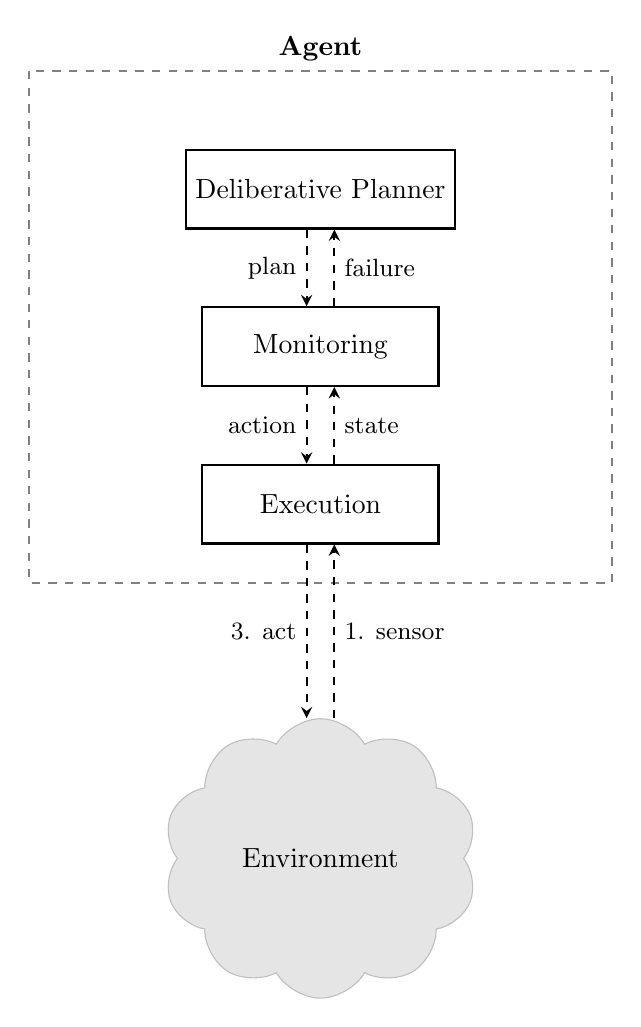
\begin{tikzpicture}[
        box/.style={rectangle, draw=black, thick, minimum width=3cm, minimum height=1cm, align=center},
        env/.style={cloud, draw=gray!50, fill=gray!20, minimum width=4cm, minimum height=2cm, cloud puffs=10, cloud puff arc=120},
        arrow/.style={->, >=stealth, dashed, thick},
        label/.style={font=\small}
    ]
    
    % Agent components (enclosed in dashed box)
    \begin{scope}[local bounding box=agent]
        % Deliberative Planner
        \node[box] (planner) at (0,2) {Deliberative Planner};
        
        % Monitoring
        \node[box] (monitoring) at (0,0) {Monitoring};
        
        % Execution
        \node[box] (execution) at (0,-2) {Execution};
    \end{scope}
    
    % Draw dashed box around agent (ending above environment)
    \draw[dashed, gray, thick] ([shift={(-2cm,1cm)}]agent.north west) rectangle ([shift={(2cm,-0.5cm)}]agent.south east);
    \node[above] at ([shift={(0,1cm)}]agent.north) {\textbf{Agent}};
    
    % Environment (outside agent boundaries)
    \node[env] (env) at (0,-6.5) {Environment};
    
    % Arrows
    % Environment to Execution (sensor) - UP arrow, goes on the right
    \draw[arrow] ([xshift=5pt]env.north) -- node[right, label] {1. sensor} ([xshift=5pt]execution.south);
    
    % Execution to Environment (act) - DOWN arrow, goes on the left
    \draw[arrow] ([xshift=-5pt]execution.south) -- node[left, label] {3. act} ([xshift=-5pt]env.north);
    
    % Execution to Monitoring (state)
    \draw[arrow] ([xshift=5pt]execution.north) -- node[right, label] {state} ([xshift=5pt]monitoring.south);
    
    % Monitoring to Execution (action)
    \draw[arrow] ([xshift=-5pt]monitoring.south) -- node[left, label] {action} ([xshift=-5pt]execution.north);
    
    % Monitoring to Deliberative Planner (failure)
    \draw[arrow] ([xshift=5pt]monitoring.north) -- node[right, label] {failure} ([xshift=5pt]planner.south);
    
    % Deliberative Planner to Monitoring (plan)
    \draw[arrow] ([xshift=-5pt]planner.south) -- node[left, label] {plan} ([xshift=-5pt]monitoring.north);
    
    \end{tikzpicture}
    \caption{Classic deliberative agent architecture (Sense-Plan-Act cycle)}
    \label{fig:deliberative_architecture}
    \end{figure}
    

The flow operates as a continuous cycle:
\begin{enumerate}
    \item The agent \textbf{senses} the environment through sensors (1. sensor), providing raw data to the Execution component.
    \item Execution updates Monitoring with the current \textbf{state}.
    \item Monitoring compares the state with the \textbf{plan} received from the Deliberative Planner and determines the next \textbf{action} for Execution. If the plan is not progressing as expected, Monitoring sends a \textbf{failure} signal to the Deliberative Planner.
    \item The Deliberative Planner receives failure signals and generates or refines a \textbf{plan}, which is sent to Monitoring.
    \item Execution \textbf{acts} (3. act) upon the environment based on the action received from Monitoring.
\end{enumerate}

This cycle represents how a deliberative agent continuously perceives, plans, and acts to achieve its goals, with a mechanism for detecting and responding to plan failures.

\subsubsection{Examples of Deliberative Architectures}

\begin{itemize}
    \item \textbf{Planning agents}: These agents use automated planning algorithms to generate sequences of actions that achieve specific goals. They maintain a symbolic representation of the world state and use search algorithms to find optimal or near-optimal plans. Planning agents are commonly used in robotics, autonomous systems, and game AI where complex sequences of actions need to be coordinated.

    \item \textbf{Belief Desire \& Intention (BDI)}: This architecture models agents based on three mental attitudes: \textbf{Beliefs} (what the agent knows about the world), \textbf{Desires} (the agent's goals or objectives), and \textbf{Intentions} (the commitments to specific plans of action). BDI agents reason about their beliefs, select desires to pursue, and commit to intentions (plans) to achieve those desires. This architecture is particularly useful for modeling complex, goal-oriented behavior in multi-agent systems and autonomous agents.
    
\end{itemize}


\subsection{Reactive Architecture}

A \textbf{reactive architecture} (also known as a \textit{behavior-based} architecture) is characterized by the agent's direct mapping from perceptions to actions without maintaining an internal world model or engaging in complex reasoning. The agent responds quickly to environmental stimuli through simple stimulus-response rules.

\textbf{Key characteristics:}
\begin{itemize}
    \item No internal world model or symbolic representation
    \item Direct mapping from sensors to actuators
    \item Simple stimulus-response rules or behaviors
    \item Fast response time
    \item Emergent behavior from simple rules
\end{itemize}

\textit{Example}: Consider a simple obstacle-avoidance robot with a reactive architecture. The robot has sensors on its front and sides, and it follows these simple rules:
\begin{itemize}
    \item If the front sensor detects an obstacle, turn right
    \item If the right sensor detects an obstacle, turn left
    \item If no obstacles are detected, move forward
    \item If both sensors detect obstacles, move backward
\end{itemize}

The robot doesn't maintain a map of its environment or plan a path. It simply reacts to what it perceives at each moment. This makes it very fast and efficient for simple tasks, though it may not find the optimal path. The robot's navigation behavior emerges from these simple reactive rules.

Figure~\ref{fig:reactive_planner_architecture} illustrates a reactive agent architecture that incorporates a \textbf{Reactive Planner} component:

\begin{itemize}
    \item \textbf{Reactive Planner}: Positioned at the top, this component generates reactive action sequences in direct response to the current state. Unlike deliberative planners, it does not maintain a complex world model but instead quickly generates actions based on immediate perceptions. It receives failure signals from Monitoring and sends actions back to Monitoring.
    \item \textbf{Monitoring}: Positioned in the middle, it monitors the execution of actions and the current state. It receives state information from Execution, sends failure signals to the Reactive Planner when deviations occur, receives actions from the Reactive Planner, and sends action commands to Execution. It also receives external plans.
    \item \textbf{Execution}: Located at the bottom, it interacts directly with the environment through sensors and actuators. It receives sensor data from the environment, updates Monitoring with the current state, receives action commands from Monitoring, and executes actions in the environment.
\end{itemize}


\begin{figure}[H]
    \centering
    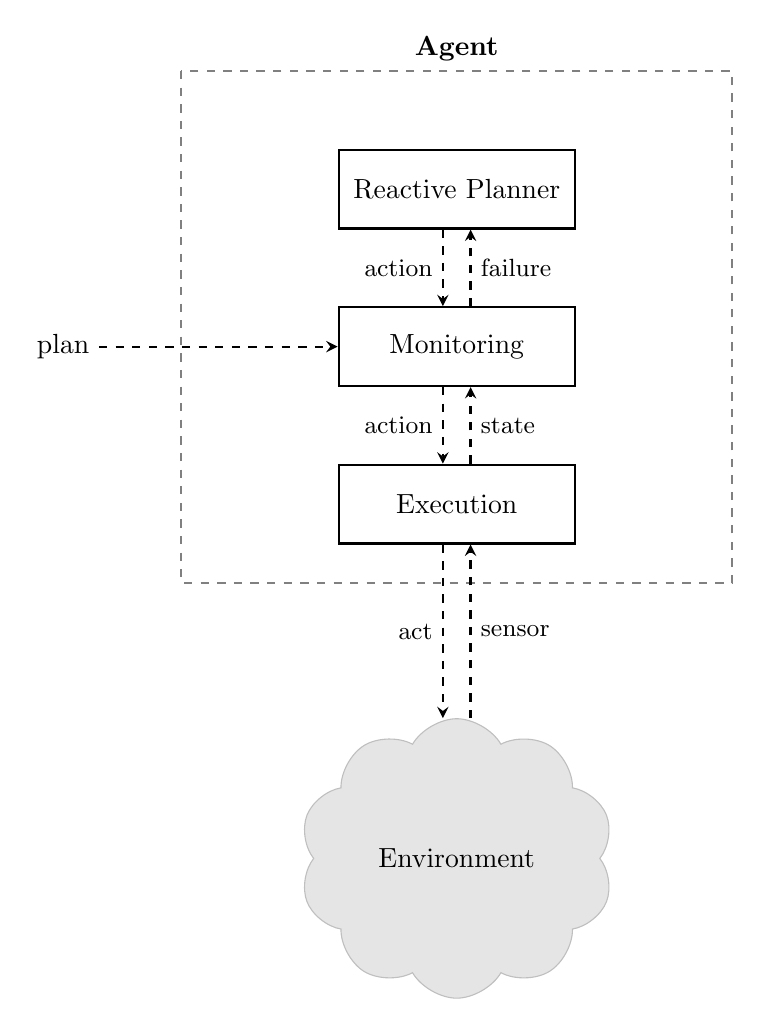
\begin{tikzpicture}[
        box/.style={rectangle, draw=black, thick, minimum width=3cm, minimum height=1cm, align=center},
        env/.style={cloud, draw=gray!50, fill=gray!20, minimum width=4cm, minimum height=2cm, cloud puffs=10, cloud puff arc=120},
        arrow/.style={->, >=stealth, dashed, thick},
        label/.style={font=\small}
    ]
    
    % Agent components (enclosed in dashed box)
    \begin{scope}[local bounding box=agent]
        % Reactive Planner (top) - centered
        \node[box] (reactive_planner) at (0,2) {Reactive Planner};
        
        % Monitoring (middle) - centered
        \node[box] (monitoring) at (0,0) {Monitoring};
        
        % Execution (bottom) - centered
        \node[box] (execution) at (0,-2) {Execution};
    \end{scope}
    
    % Draw dashed box around agent (ending above environment)
    \draw[dashed, gray, thick] ([shift={(-2cm,1cm)}]agent.north west) rectangle ([shift={(2cm,-0.5cm)}]agent.south east);
    \node[above] at ([shift={(0,1cm)}]agent.north) {\textbf{Agent}};
    
    % Plan source (outside agent boundaries, to the left of monitoring)
    \node (plan_source) at (-5,0) {plan};
    
    % Environment (outside agent boundaries)
    \node[env] (env) at (0,-6.5) {Environment};
    
    % Arrows
    % Plan to Monitoring
    \draw[arrow] (plan_source.east) -- node[above, label] {} (monitoring.west);
    
    % Environment to Execution (sensor) - UP arrow, goes on the right
    \draw[arrow] ([xshift=5pt]env.north) -- node[right, label] {sensor} ([xshift=5pt]execution.south);
    
    % Execution to Environment (act) - DOWN arrow, goes on the left
    \draw[arrow] ([xshift=-5pt]execution.south) -- node[left, label] {act} ([xshift=-5pt]env.north);
    
    % Execution to Monitoring (state)
    \draw[arrow] ([xshift=5pt]execution.north) -- node[right, label] {state} ([xshift=5pt]monitoring.south);
    
    % Monitoring to Reactive Planner (failure)
    \draw[arrow] ([xshift=5pt]monitoring.north) -- node[right, label] {failure} ([xshift=5pt]reactive_planner.south);
    
    % Reactive Planner to Monitoring (action)
    \draw[arrow] ([xshift=-5pt]reactive_planner.south) -- node[left, label] {action} ([xshift=-5pt]monitoring.north);
    
    % Monitoring to Execution (action)
    \draw[arrow] ([xshift=-5pt]monitoring.south) -- node[left, label] {action} ([xshift=-5pt]execution.north);
    
    \end{tikzpicture}
    \caption{Reactive agent architecture with Reactive Planner}
    \label{fig:reactive_planner_architecture}
    \end{figure}



The flow operates as follows:
\begin{enumerate}
    \item An external \textbf{plan} is provided to the Monitoring component (this could come from a higher-level planner or user input).
    \item The Environment sends \textbf{sensor} data to the Execution component, providing raw information about the current state of the environment.
    \item Execution processes the sensor data and updates Monitoring with the current \textbf{state}.
    \item Monitoring evaluates the state against the plan. If there is a deviation or problem, it sends a \textbf{failure} signal to the Reactive Planner.
    \item The Reactive Planner receives the failure signal and immediately generates a reactive \textbf{action} response, which it sends back to Monitoring.
    \item Monitoring receives the action from the Reactive Planner and forwards the \textbf{action} command to Execution.
    \item Execution \textbf{acts} upon the environment based on the action received from Monitoring.
\end{enumerate}

This architecture emphasizes fast, reactive responses to environmental changes while still allowing for external plan guidance. The Reactive Planner provides quick adaptation without the overhead of maintaining complex internal models. The bidirectional flow between Monitoring and the Reactive Planner enables rapid failure detection and action generation.

\subsubsection{Examples of Reactive Architectures}

\begin{itemize}
    \item \textbf{Subsumption architecture}: A layered architecture where behaviors are organized in levels of increasing complexity. Lower-level behaviors (like obstacle avoidance) can subsume or override higher-level behaviors (like exploration) when triggered by environmental conditions. Each layer operates independently and reactively, with no central control or world model.
    
    \item \textbf{Agent network architecture from Pattie Maes}: A distributed reactive architecture where multiple simple agents (or behaviors) are connected in a network. Each agent has local rules and can activate or inhibit other agents. The overall behavior emerges from the interactions between these agents, without centralized planning.
    
    \item \textbf{Reactive execution model}: Is domain independent and operates with structures precalculated at runtime.
\end{itemize}

\subsection{Hybrid Architecture}
\label{subsec:hybrid}

A \textbf{hybrid architecture} combines elements of both deliberative and reactive architectures. It typically has multiple layers: a reactive layer for fast, immediate responses to critical situations, and a deliberative layer for complex planning and reasoning. This architecture attempts to get the best of both worlds: the speed of reactive systems and the intelligence of deliberative systems.

\textbf{Key characteristics:}
\begin{itemize}
    \item Combines reactive and deliberative components
    \item Multiple layers of control (reactive at the bottom, deliberative at the top)
    \item Fast response for urgent situations (reactive layer)
    \item Complex reasoning and planning for strategic decisions (deliberative layer)
    \item Coordination between layers
\end{itemize}

\textit{Example}: Consider an autonomous vehicle with a hybrid architecture. The vehicle has two main layers:

\begin{itemize}
    \item \textbf{Reactive layer}: Handles immediate, critical situations. For example:
    \begin{itemize}
        \item If a pedestrian suddenly appears in front, immediately apply brakes (no time for planning)
        \item If another vehicle swerves into the lane, quickly adjust steering
    \end{itemize}
    
    \item \textbf{Deliberative layer}: Handles strategic planning and navigation. For example:
    \begin{itemize}
        \item Plans the route from origin to destination
        \item Analyzes traffic conditions and selects the best path
        \item Decides when to change lanes based on traffic patterns
        \item Maintains a map and tracks the vehicle's position
    \end{itemize}
\end{itemize}

The reactive layer ensures safety by responding instantly to immediate threats, while the deliberative layer handles the overall navigation strategy. The layers work together: the deliberative layer sets the general plan, and the reactive layer handles unexpected situations that require immediate action.

\subsubsection{Examples of Hybrid Architectures}

\begin{itemize}
    \item \textbf{Procedural Reasoning System (PRS)}: A BDI (Belief-Desire-Intention) architecture that combines deliberative reasoning with reactive capabilities. The agent maintains \textbf{Beliefs} (facts about the world expressed in first-order logic), \textbf{Desires} (system behaviors or goals), and \textbf{Intentions} (the current set of active plans). PRS includes a library of partially specified plans called Knowledge Areas (KAs), each with an activation condition. KAs can be activated by goals or by data, and can be reactive, allowing PRS to respond quickly to environmental changes while also reasoning about which plans to execute.
    
    \item \textbf{COSY (Cooperative System)}: A BDI architecture that combines elements from both PRS and IRMA architectures. It has five main components: \textbf{Sensors} (receive perceptual inputs), \textbf{Actuators} (perform actions), \textbf{Communications} (send messages), \textbf{Cognition} (mediates between intentions and knowledge to choose actions), and \textbf{Intention} (contains long-term goals and control elements). COSY combines deliberative reasoning with reactive communication and action capabilities, making it suitable for interactive and collaborative environments.
\end{itemize}


\subsection{Cognitive Architecture}

A \textbf{cognitive architecture} is a computational framework that models the structure and processes of human cognition. It provides a unified theory of how the mind works, including perception, memory, reasoning, learning, and decision-making. Cognitive architectures can be defined as a hypothesis about the fixed structures that provide a mind, whether in natural or artificial systems, and how they work together—along with the knowledge and skills incorporated within the architecture—to produce intelligent behavior in a diversity of complex environments. Cognitive architectures aim to create artificial agents that can exhibit human-like intelligence and behavior.

\textbf{Key characteristics:}
\begin{itemize}
    \item Models human cognitive processes and structures
    \item Provides unified framework for multiple cognitive functions
    \item Includes memory systems (short-term and long-term)
    \item Supports learning and adaptation
    \item Integrates perception, reasoning, and action
    \item Based on cognitive science and psychology principles
\end{itemize}

\subsubsection{Examples of Cognitive Architectures}

\begin{itemize}
    \item \textbf{ACT-R}: A cognitive architecture developed primarily by John Robert Anderson at Carnegie Mellon University. The most important assumption of ACT-R is that human knowledge can be divided into two irreducible types of representations:
    \begin{itemize}
        \item \textbf{Declarative knowledge}: Represented as \textbf{chunks} (vector representations of individual properties, each accessible from a labeled slot)
        \item \textbf{Procedural knowledge}: Represented as production rules
    \end{itemize}
    Chunks are maintained and accessed through \textbf{buffers}, which are the front-end of \textbf{modules} (specialized and largely independent brain structures). ACT-R has two main types of modules:
    \begin{itemize}
        \item \textbf{Perceptual-motor module}: Handles interaction with the environment, managing the flow of perception and action necessary to connect the agent with the world
        \item \textbf{Memory module}: Divided into:
        \begin{itemize}
            \item \textbf{Long-term memory} (production memory): Contains production rules
            \item \textbf{Short-term memory} (working memory or declarative memory): Contains current facts about the world
        \end{itemize}
    \end{itemize}
     
    \item \textbf{SOAR}: A cognitive architecture created at Carnegie Mellon University by Laird, Newell, and Rosenbloom (1987). The ultimate goal of SOAR is to provide a foundation for a system capable of general intelligent behavior, supporting the full range of cognitive tasks, problem-solving methods, and knowledge representations. SOAR is both a theory of cognition and a computational implementation of that theory.
    
    The design of SOAR is based on the hypothesis that all goal-oriented deliberate behavior can be understood as the selection and application of \textbf{operators} to a \textbf{state}:
    \begin{itemize}
        \item \textbf{State}: A representation of the current problem situation
        \item \textbf{Operator}: Transforms a state (performs changes in the representation)
        \item \textbf{Goal}: A desired result for the problem
    \end{itemize}
    SOAR runs continuously, attempting to apply the current operator and select the next operator (a state can have only one operator at a time) until the goal is achieved.
    
    SOAR has separate memories with different representation modes:
    \begin{itemize}
        \item \textbf{Short-term memory}: Stores sensor data, intermediate inferences about current data, currently active goals, and active operators (actions and plans)
        \item \textbf{Long-term memory} (production memory): Maintains knowledge for responding to situations through procedures. It stores problem-solving knowledge, inference rules, and knowledge for selecting and applying operators in specific states
    \end{itemize}
\end{itemize}


\subsection{Other Architectures}

\begin{itemize}
    \item Three layer architecture
    \item Multilayer architecture
    \item Three tower architecture
\end{itemize}




\clearpage
\section{Summary - Lecture 001}
\begin{figure}[H]
\centering
\resizebox{1\textwidth}{!}{
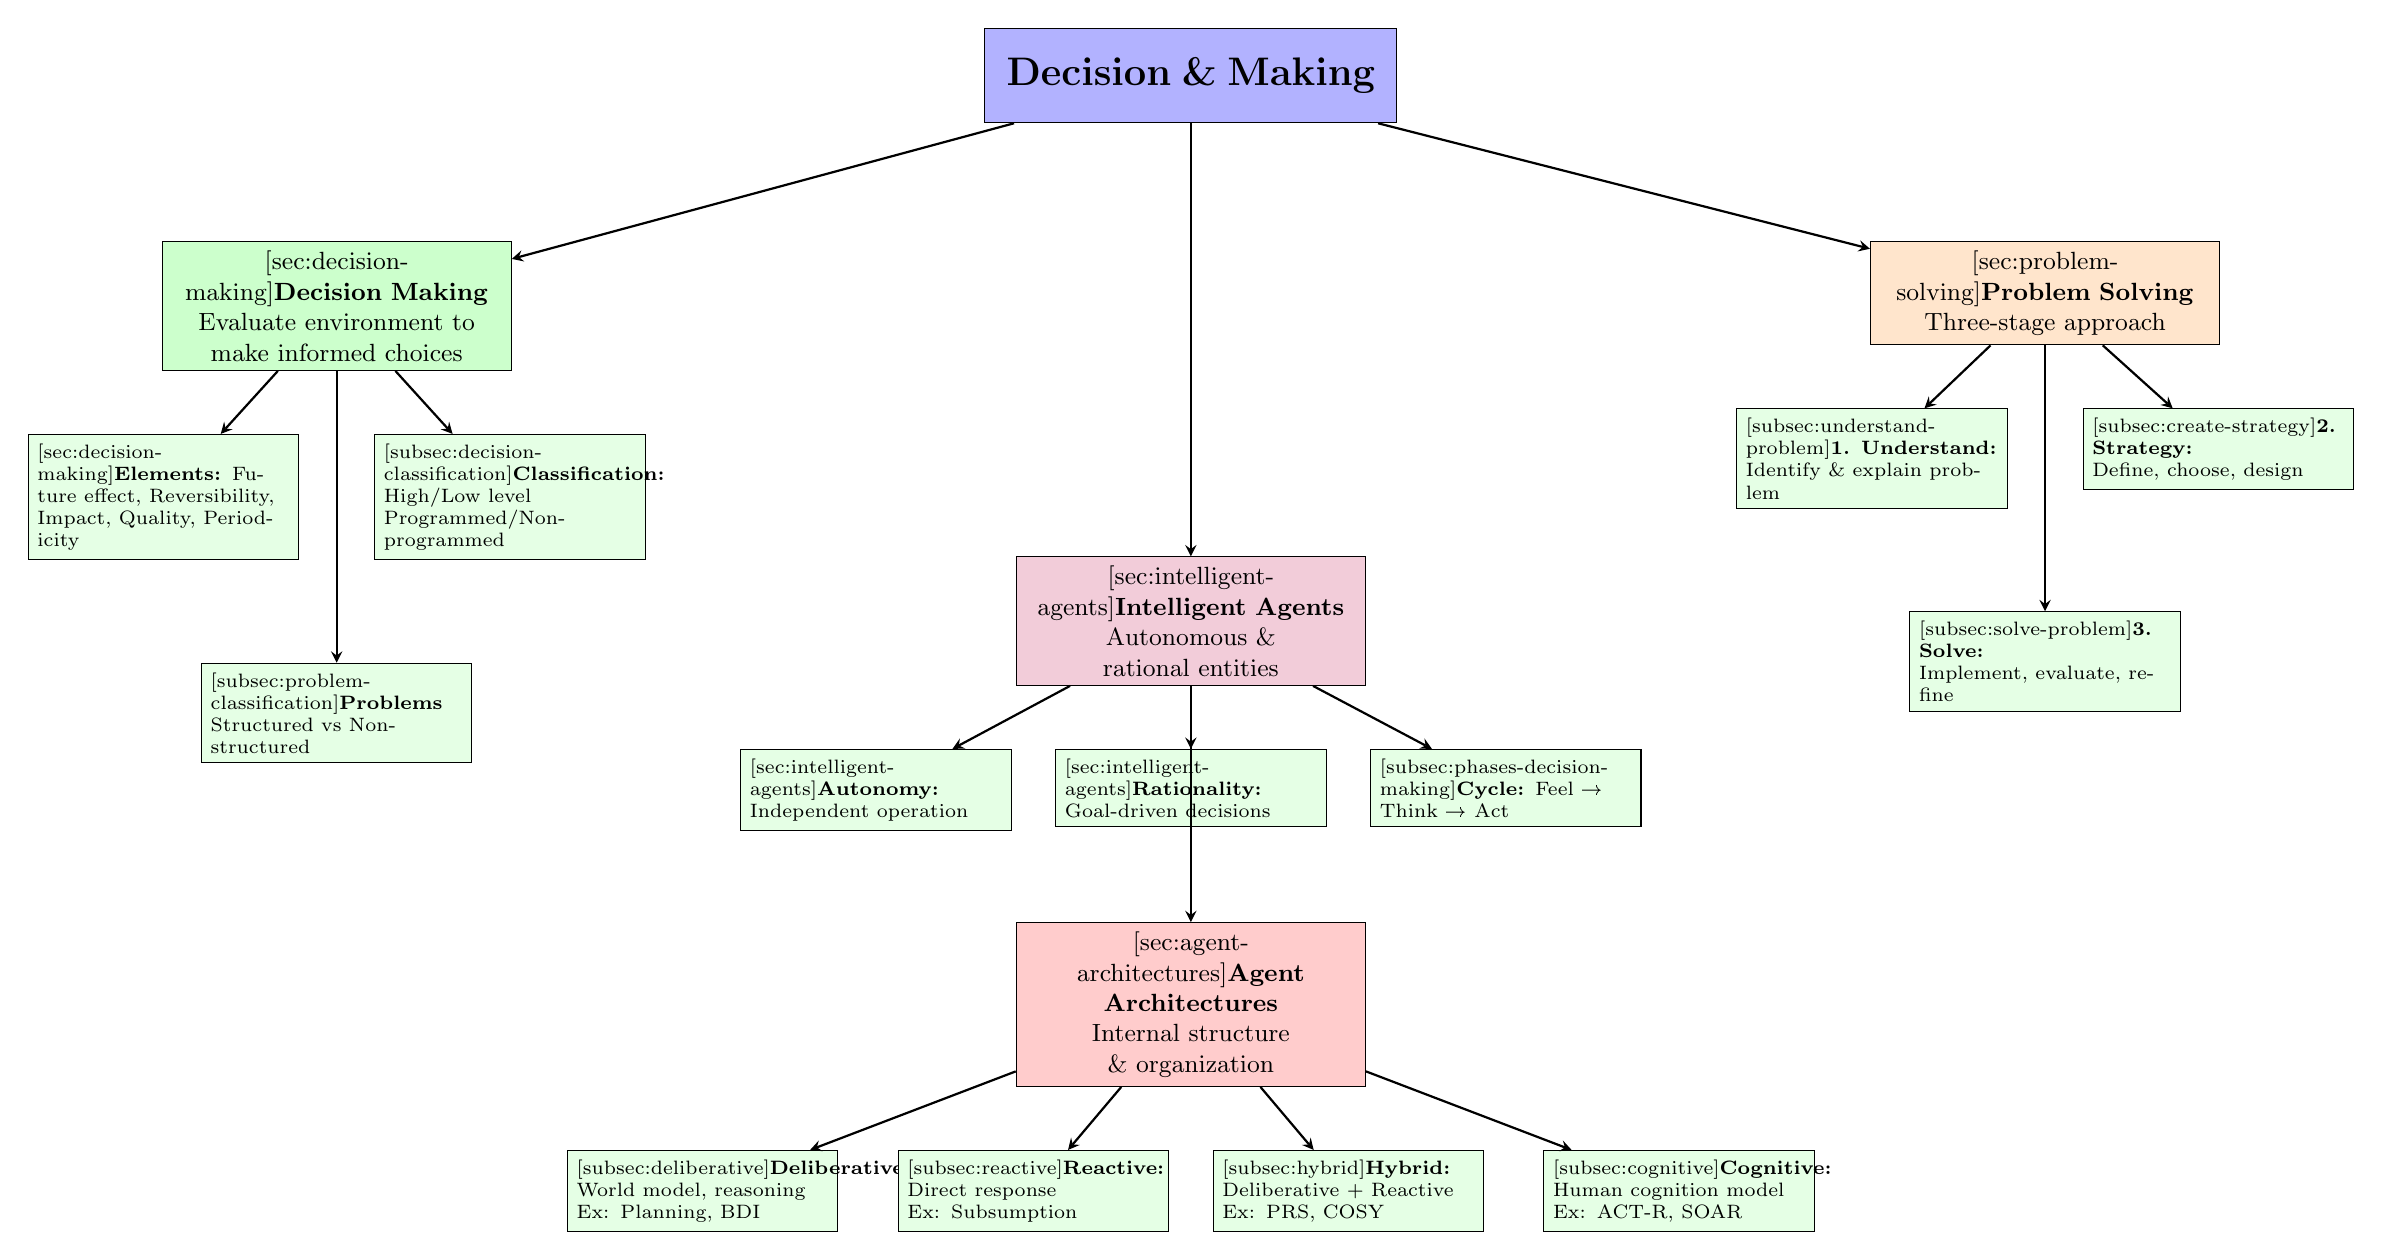
\begin{tikzpicture}[
    node distance=1.5cm and 2cm,
    box/.style={rectangle, draw, fill=blue!10, text width=4.2cm, align=center, minimum height=1cm, font=\small},
    titlebox/.style={rectangle, draw, fill=blue!30, text width=5cm, align=center, minimum height=1.2cm, font=\bfseries},
    smallbox/.style={rectangle, draw, fill=green!10, text width=3.2cm, align=left, minimum height=0.8cm, font=\scriptsize},
    arrow/.style={->, >=stealth, thick}
]

% Main title
\node[titlebox] (main) at (0,0) {\Large Decision \& Making};

% Decision Making section
\node[box, fill=green!20, below left=of main, xshift=-4cm] (dm) {\hyperref[sec:decision-making]{\textbf{Decision Making}}\\Evaluate environment to make informed choices};
\node[smallbox, below=0.8cm of dm, xshift=-2.2cm] (dm-elem) {\hyperref[sec:decision-making]{\textbf{Elements:}} Future effect, Reversibility, Impact, Quality, Periodicity};
\node[smallbox, below=0.8cm of dm, xshift=2.2cm] (dm-class) {\hyperref[subsec:decision-classification]{\textbf{Classification:}}\\High/Low level\\Programmed/Non-programmed};
\node[smallbox, below=0.8cm of dm-elem, yshift=-0.5cm, xshift=2.2cm] (prob-class) {\hyperref[subsec:problem-classification]{\textbf{Problems}}\\Structured vs Non-structured};

% Problem Solving section
\node[box, fill=orange!20, below right=of main, xshift=4cm] (ps) {\hyperref[sec:problem-solving]{\textbf{Problem Solving}}\\Three-stage approach};
\node[smallbox, below=0.8cm of ps, xshift=-2.2cm] (ps1) {\hyperref[subsec:understand-problem]{\textbf{1. Understand:}}\\Identify \& explain problem};
\node[smallbox, below=0.8cm of ps, xshift=2.2cm] (ps2) {\hyperref[subsec:create-strategy]{\textbf{2. Strategy:}}\\Define, choose, design};
\node[smallbox, below=0.8cm of ps1, yshift=-0.5cm, xshift=2.2cm] (ps3) {\hyperref[subsec:solve-problem]{\textbf{3. Solve:}}\\Implement, evaluate, refine};

% Intelligent Agents section
\node[box, fill=purple!20, below=5.5cm of main] (ia) {\hyperref[sec:intelligent-agents]{\textbf{Intelligent Agents}}\\Autonomous \& rational entities};
\node[smallbox, below=0.8cm of ia, xshift=-4cm] (ia-auto) {\hyperref[sec:intelligent-agents]{\textbf{Autonomy:}}\\Independent operation};
\node[smallbox, below=0.8cm of ia] (ia-rat) {\hyperref[sec:intelligent-agents]{\textbf{Rationality:}}\\Goal-driven decisions};
\node[smallbox, below=0.8cm of ia, xshift=4cm] (ia-cycle) {\hyperref[subsec:phases-decision-making]{\textbf{Cycle:}} Feel → Think → Act};

% Agent Architectures section
\node[box, fill=red!20, below=3cm of ia] (arch) {\hyperref[sec:agent-architectures]{\textbf{Agent Architectures}}\\Internal structure \& organization};

\node[smallbox, below=0.8cm of arch, xshift=-6.2cm] (delib) {\hyperref[subsec:deliberative]{\textbf{Deliberative:}}\\World model, reasoning\\Ex: Planning, BDI};
\node[smallbox, below=0.8cm of arch, xshift=-2cm] (react) {\hyperref[subsec:reactive]{\textbf{Reactive:}}\\Direct response\\Ex: Subsumption};
\node[smallbox, below=0.8cm of arch, xshift=2cm] (hybrid) {\hyperref[subsec:hybrid]{\textbf{Hybrid:}}\\Deliberative + Reactive\\Ex: PRS, COSY};
\node[smallbox, below=0.8cm of arch, xshift=6.2cm] (cogn) {\hyperref[subsec:cognitive]{\textbf{Cognitive:}}\\Human cognition model\\Ex: ACT-R, SOAR};

% Arrows
\draw[arrow] (main) -- (dm);
\draw[arrow] (main) -- (ps);
\draw[arrow] (main) -- (ia);
\draw[arrow] (ia) -- (arch);

\draw[arrow] (dm) -- (dm-elem);
\draw[arrow] (dm) -- (dm-class);
\draw[arrow] (dm) -- (prob-class);

\draw[arrow] (ps) -- (ps1);
\draw[arrow] (ps) -- (ps2);
\draw[arrow] (ps) -- (ps3);

\draw[arrow] (ia) -- (ia-auto);
\draw[arrow] (ia) -- (ia-rat);
\draw[arrow] (ia) -- (ia-cycle);

\draw[arrow] (arch) -- (delib);
\draw[arrow] (arch) -- (react);
\draw[arrow] (arch) -- (hybrid);
\draw[arrow] (arch) -- (cogn);

\end{tikzpicture}
}
\caption{Conceptual map of the Reasoning and Planning course - Lecture 001}
\end{figure}



% Lecture 002
\section*{Lecture 002}
\section{Symbolic Representation of Knowledge}
\label{sec:symbolic-representation}

When agents make decisions based on changes in the environment, a fundamental question arises: \textbf{how do we represent the environment and the problem's information?} Agents need a way to understand and work with information about the world, which is where symbolic representation becomes essential.

Reasoning is an internal process that operates on external entities. The key insight is that \textbf{operations with representations substitute operations with the real world}. Instead of directly interacting with the environment, agents can manipulate symbolic representations of it, allowing them to reason about possible actions and outcomes before actually taking action.

Symbolic representation allows agents to create \textbf{internal models of the external world using symbols} (such as variables, predicates, logical formulas, or other formal structures). These representations enable reasoning processes that can:
\begin{itemize}
    \item \textbf{Simulate} different scenarios and outcomes
    \item \textbf{Predict} the consequences of actions
    \item \textbf{Plan} sequences of actions before execution
    \item \textbf{Learn} from experience without direct interaction
\end{itemize}

This makes decision-making more efficient and safer, as agents can explore possibilities and evaluate strategies in a controlled, internal environment before committing to actions in the real world. It is important to note that reasoning and action are \textbf{complementary} rather than substitutes: reasoning often precedes and guides action, enabling agents to make informed decisions rather than acting randomly.

\subsection{Requirements for Knowledge Representation}
\label{subsec:requirements-representation}

According to \citep{upm14207} a knowledge representation must satisfy:

\begin{enumerate}
    \item \textbf{Formal}: The representation must be unambiguous. Natural language is not considered a knowledge representation because of its ambiguities.
    
    \textit{Example}: The sentence "I saw the man with binoculars" is ambiguous—it could mean "I used binoculars to see the man" or "I saw the man who had binoculars." A formal representation would explicitly distinguish these meanings, such as \texttt{Saw(I, man) $\land$ Used(I, binoculars)} versus \texttt{Saw(I, man) $\land$ Has(man, binoculars)}.
    
    \item \textbf{Expressive}: The representation must be rich enough to capture the different aspects that need to be distinguished. For example, first-order predicate logic formulas are more expressive than propositional calculus.
    
    \textit{Example}: Propositional logic can only express simple statements like "It is raining" (P) or "The ground is wet" (Q). Predicate logic can express relationships and quantification, such as \texttt{$\forall$x (Bird(x) $\rightarrow$ CanFly(x))} meaning "All birds can fly," or \texttt{Loves(john, mary)} expressing the relationship "John loves Mary."
    
    \item \textbf{Natural}: The representation should be sufficiently analogous to natural ways of expressing knowledge. Traditional quantitative mathematical representations (e.g., matrices) can be too artificial for emulating reasoning processes.
    
    \textit{Example}: Representing "John loves Mary" as a matrix entry (row 1, column 2 = 1) is mathematically precise but doesn't match how humans naturally think about relationships. A more natural representation would be a semantic network with nodes and edges: \texttt{[John] --loves--> [Mary]}, or a frame structure with properties, which aligns better with human cognitive patterns.
    
    \item \textbf{Tractable}: The representation must be computationally tractable, meaning there must exist sufficiently efficient procedures to generate answers through manipulation of the knowledge base elements.
    
    \textit{Example}: While a representation might be perfectly formal and expressive, if answering queries requires exponential time or is undecidable, it becomes impractical. For instance, certain logical formalisms may be too complex to reason about efficiently, making them unsuitable for real-time applications despite their theoretical expressiveness.
\end{enumerate}

It is important to note that "natural" in this context refers to \textbf{cognitive naturalness}—how well the representation aligns with human thinking patterns—not to natural language. Natural language is ambiguous and therefore not formal, while we seek representations that are both formal (unambiguous) and natural (intuitive). The ideal representation balances both requirements.

In general, it is convenient to create information representations based on a \textbf{single representation}. This approach improves knowledge base maintenance, as it provides consistency and simplifies updates across the system.

\textit{Example}: A system might use only first-order predicate logic to represent all knowledge:
\begin{itemize}
    \item Facts: \texttt{Student(john)}, \texttt{Course(cs101)}, \texttt{Enrolled(john, cs101)}
    \item Rules: \texttt{$\forall$x (Student(x) $\land$ Enrolled(x, y) $\rightarrow$ TakesCourse(x, y))}
    \item Relationships: \texttt{Teaches(profSmith, cs101)}, \texttt{Prerequisite(cs101, cs201)}
\end{itemize}
Alternatively, a system might use only semantic networks, representing everything as nodes and edges: \texttt{[John] --is\_a--> [Student]}, \texttt{[John] --enrolled\_in--> [CS101]}, etc.

However, in some cases, attempting to represent all knowledge in a single representation can \textbf{limit the application of techniques and algorithms}. Different problems and subtasks may require different representation formalisms or specialized techniques that are not well-suited to a unified representation.

For complex systems that require making decisions at different levels, it is common to employ the idea of generating \textbf{multi-layer agents} \citep{upm14207} that decompose the problem into levels. For each level, a treatment is established oriented to a specialized agent that needs a \textbf{concrete representation of part of the environment information}. Each agent at its respective layer uses a representation tailored to its specific needs and the techniques it employs.

\subsection{Types of Knowledge}
\label{subsec:types-knowledge}

To solve problems in a natural way, it is necessary to carry out a precise analysis of knowledge. For this, we must take into account the different classifications of knowledge used in artificial intelligence \citep{upm14207}. The main types of knowledge are:

\begin{enumerate}
    \item \textbf{Domain Knowledge}: Knowledge about a specific context or problem, represented in a \textbf{declarative} way (describes what exists, properties, and constraints). It can be incomplete and does not require order or relationships between elements.
    
    \item \textbf{Explicit Knowledge}: \textbf{Knowledge extracted from introspective analysis of one's own reasoning and problem-solving processes}. It is usually expressed through frames or rules about how problems are solved.
    
    \item \textbf{Implicit Knowledge}: Knowledge about innate capacities or abilities that are not easily expressed verbally. Bayesian networks or neural networks are used for its representation or modeling.
    
    \item \textbf{Superficial Knowledge}: Knowledge obtained through experience in solving similar problems. It uses practical rules or heuristics that work but don't explain the underlying theoretical principles.
    
    \item \textbf{Deep Knowledge}: Knowledge based on a well-structured theoretical framework that explains the underlying principles and mechanisms in detail. However, it is not present in many problems because it is not easy to have a theoretical analysis of the environment's functioning in all problems.
    
    \item \textbf{Control Knowledge}: The \textbf{strategy/organization for the problem-solving process} — the execution order and approach for how to solve the problem, not just the steps of the task itself. In many cases, it can lead to coding a program in the expansion sequence of search algorithms.
    
    \item \textbf{Metaknowledge}: \textbf{Knowledge about how to generate, transfer, and learn from knowledge}. It allows generating new models from previous problem models and establishes relationships between levels of knowledge bases.
\end{enumerate}
\section{Introduction to Reasoning}
\label{sec:introduction-reasoning}

Reasoning refers to a set of mental activities that connect ideas based on rules that justify an idea, allowing problem-solving through conclusions.



As can be observed in these definitions, all authors refer to the same concepts: \textbf{premises} (initial propositions, what is already known) and \textbf{conclusion} (final proposition obtained from the premises, representing new knowledge).

\subsection{Elements of Reasoning: Content and Form}
\label{subsec:content-form}

In all reasoning, there exist two elements: \textbf{content} and \textbf{form}.

\begin{itemize}
    \item \textbf{Content}: What makes a proposition true or false. It is the reference to objects and properties. Content deals with the actual meaning and truth value of statements in the real world.
    
    \textit{Example}: In the proposition "It is raining," the content refers to the actual weather condition. This proposition can be true or false depending on whether it is actually raining.
    
    \item \textbf{Form}: The logical connection between the antecedents (what is already known, the premises) and the consequents (the conclusion inferred from the antecedents). This connection that implies inference is expressed through conjunctions. Form is what makes the proposition \textbf{valid}, and consists of using symbols to express the validity of propositions. Form deals with the logical structure of reasoning, independent of whether the statements are actually true or false.
    
    \textit{Example}: Consider the following reasoning:
    \begin{itemize}
        \item Premise 1: "If it rains, then the ground gets wet"
        \item Premise 2: "It is raining"
        \item Conclusion: "Therefore, the ground gets wet"
    \end{itemize}
    The form of this reasoning is: \texttt{If P, then Q. P. Therefore, Q.} This logical structure is valid regardless of whether it is actually raining or not. The same form can be applied to different content:
    \begin{itemize}
        \item Premise 1: "If John is a student, then John studies"
        \item Premise 2: "John is a student"
        \item Conclusion: "Therefore, John studies"
    \end{itemize}
    Both examples share the same valid logical form, even though they have different content.
\end{itemize}

The distinction between content and form is crucial: \textbf{content} determines whether propositions are true or false in the real world, while \textbf{form} determines whether the reasoning structure is valid (whether the conclusion follows logically from the premises).

We speak of \textbf{valid reasoning} when the conclusion follows from the premises. A reasoning is considered valid based on its logical form, even if the conclusion or the premises are false. On the other hand, \textbf{invalid reasoning} occurs when, from true premises, a false conclusion is obtained.

Table~\ref{tab:validity-reasoning} shows the different scenarios for reasoning validity based on the truth values of premises and conclusion:

\begin{table}[H]
\centering
\caption{Validity or Non-Validity of a Reasoning}
\label{tab:validity-reasoning}
\begin{tabular}{p{5cm}p{4cm}p{4cm}}
\toprule
\textbf{If the premises are...} & \textbf{And the conclusion is...} & \textbf{The reasoning is...} \\
\midrule
True & True & \textcolor{green}{Valid} \\
\midrule
\rowcolor{gray!30}
True & False & \textcolor{red}{Invalid} \\
\midrule
False & True & \textcolor{green}{Valid} \\
\midrule
False & False & \textcolor{green}{Valid} \\
\bottomrule
\end{tabular}
\end{table}

The concept of reasoning validity is directly analogous to the truth conditions of a conditional proposition. Table~\ref{tab:conditional-truth} shows the truth table for a conditional proposition (p → q), where p represents the premises (antecedent) and q represents the conclusion (consequent):

\begin{table}[H]
\centering
\caption{Truth Table of a Conditional Proposition}
\label{tab:conditional-truth}
\begin{tabular}{ccc}
\toprule
\textbf{p} & \textbf{q} & \textbf{p → q} \\
\midrule
1 (True) & 1 (True) & 1 (True) \\
\midrule
\rowcolor{gray!30}
1 (True) & 0 (False) & 0 (False) \\
\midrule
0 (False) & 1 (True) & 1 (True) \\
\midrule
0 (False) & 0 (False) & 1 (True) \\
\bottomrule
\end{tabular}
\end{table}

As can be observed, the highlighted row in both tables (premises True, conclusion False) represents the only scenario where the reasoning is invalid and the conditional proposition is false. This emphasizes that an argument is invalid if and only if it is possible for its premises to be true and its conclusion false.

The following examples illustrate each scenario from Table~\ref{tab:validity-reasoning}:

\begin{enumerate}
    \item \textbf{True premises → True conclusion (Valid)}:
    \begin{itemize}
        \item Premise 1: "If it rains, then the ground gets wet" (True)
        \item Premise 2: "It is raining" (True)
        \item Conclusion: "Therefore, the ground is wet" (True)
    \end{itemize}
    This reasoning is \textbf{valid} because the conclusion follows logically from the premises (modus ponens), and all statements are true.
    
    \item \textbf{True premises → False conclusion (Invalid)}:
    \begin{itemize}
        \item Premise 1: "All dogs are animals" (True)
        \item Premise 2: "Lassie is an animal" (True)
        \item Conclusion: "Therefore, Lassie is a dog" (False - Lassie could be any animal)
    \end{itemize}
    This reasoning is \textbf{invalid} because the conclusion does not follow from the premises (fallacy of affirming the consequent). Even though the premises are true, the logical form is incorrect, making it possible for the conclusion to be false.
    
    \item \textbf{False premises → True conclusion (Valid)}:
    \begin{itemize}
        \item Premise 1: "If it is July, then it is winter" (False - in the Northern Hemisphere)
        \item Premise 2: "It is July" (False - assume it is actually January)
        \item Conclusion: "Therefore, it is winter" (True - it is winter in January)
    \end{itemize}
    This reasoning is \textbf{valid} because the logical form (modus ponens) is correct, even though both premises are false and the conclusion happens to be true. The validity depends on the form, not the truth values.
    
    \item \textbf{False premises → False conclusion (Valid)}:
    \begin{itemize}
        \item Premise 1: "All insects are mammals" (False)
        \item Premise 2: "Spiders are insects" (False - spiders are arachnids)
        \item Conclusion: "Therefore, spiders are mammals" (False)
    \end{itemize}
    This reasoning is \textbf{valid} because the conclusion follows logically from the premises using a valid syllogistic form. Even though both premises and the conclusion are false, the logical structure is correct—if the premises were true, the conclusion would necessarily follow.
\end{enumerate}

\section{Reasoning Classification}
\label{sec:reasoning-classification}

Although there are many types of reasoning, we will focus on the most important ones for artificial intelligence: \textbf{deductive}, \textbf{inductive}, and \textbf{abductive} reasoning.

\subsection{Deductive Reasoning}
\label{subsec:deductive-reasoning}

Reasoning is \textbf{deductive} when it requires that the conclusion necessarily and forcibly derives from the premises. For this reason, it is considered rigorous.

\textit{Example of deductive reasoning}:
\begin{itemize}
    \item "If it snows, then it is cold"
    \item "It is snowing"
    \item "Therefore, I am cold"
\end{itemize}

It is understood that validity exists when, from true premises, a false conclusion cannot be obtained. From false premises, true conclusions can be derived, and yet the argument can still be valid.

\textbf{Truth} occurs when what is described in the premises corresponds to reality. This type of reasoning goes from \textbf{general to particular}.

\subsubsection{Types of Deductive Reasoning}
\label{subsubsec:types-deductive}

Within deductive reasoning, several types are distinguished:

\begin{itemize}
    \item \textbf{Categorical deductive reasoning}: Starts from two true premises that will lead to a true conclusion.
    
    \textit{Example}:
    \begin{itemize}
        \item Premise 1: "All humans are mortal" (True)
        \item Premise 2: "Socrates is a human" (True)
        \item Conclusion: "Therefore, Socrates is mortal" (True)
    \end{itemize}
    
    \item \textbf{Propositional deductive reasoning}: Relates two premises where one is a condition of the other, antecedent and consequent.
    
    \textit{Example}:
    \begin{itemize}
        \item Premise 1: "If it rains, then the ground gets wet" (antecedent: it rains, consequent: ground gets wet)
        \item Premise 2: "It is raining" (antecedent is true)
        \item Conclusion: "Therefore, the ground is wet" (consequent follows)
    \end{itemize}
    
    \item \textbf{Disjunction or dilemma}: The relationship between the premises is one of contraries, therefore the conclusion discards one of them.
    
    \textit{Example}:
    \begin{itemize}
        \item Premise 1: "Either it is day or it is night"
        \item Premise 2: "It is not day"
        \item Conclusion: "Therefore, it is night" (discards the first option)
    \end{itemize}
\end{itemize}

\subsubsection{Forms of Deductive Reasoning}
\label{subsubsec:forms-deductive}

There are two forms of deductive reasoning:

\begin{itemize}
    \item \textbf{Immediate}: The only logical operation is the change of judgment.
    
    \textit{Example}:
    \begin{itemize}
        \item Original judgment: "All students are learners"
        \item Immediate conclusion: "No students are non-learners" (direct conversion/transformation of the same judgment)
    \end{itemize}
    In immediate reasoning, the conclusion is obtained directly from a single premise by changing its form, without needing additional premises.
    
    \item \textbf{Mediate}: A mediation relationship is established between judgments to reach the conclusion.
    
    \textit{Example}:
    \begin{itemize}
        \item Premise 1: "All mammals are warm-blooded"
        \item Premise 2: "All dogs are mammals" (middle term: "mammals")
        \item Conclusion: "Therefore, all dogs are warm-blooded"
    \end{itemize}
    In mediate reasoning, the conclusion is reached by connecting two premises through a middle term (in this case, "mammals"), which mediates the relationship between the other terms.
\end{itemize}

The deductive method goes from \textbf{general to particular}. Table~\ref{tab:syllogism-example} illustrates a classic syllogism example:

\begin{table}[H]
\centering
\caption{Example of a syllogism}
\label{tab:syllogism-example}
\begin{tabular}{p{3cm}p{3cm}p{5cm}}
\toprule
\textbf{Part} & \textbf{Abbreviation} & \textbf{Statement} \\
\midrule
Major Premise & MP & Humans are mortal. \\
\midrule
Minor Premise & SM & Greeks are humans. \\
\midrule
Conclusion & SP & Greeks are mortal. \\
\bottomrule
\end{tabular}
\end{table}

In syllogistic logic, the abbreviations follow a standard terminology:
\begin{itemize}
    \item \textbf{S (Subject)}: The subject of the conclusion ("Greeks")
    \item \textbf{P (Predicate)}: The predicate of the conclusion ("mortal")
    \item \textbf{M (Middle)}: The term that appears in both premises but not in the conclusion ("humans")
\end{itemize}

In this syllogism:
\begin{itemize}
    \item \textbf{Major Premise (MP)}: Contains the Major Term (P = "mortal") and Middle Term (M = "humans")
    \item \textbf{Minor Premise (SM)}: Contains the Minor Term (S = "Greeks") and Middle Term (M = "humans")
    \item \textbf{Conclusion (SP)}: Contains the Minor Term (S = "Greeks") and Major Term (P = "mortal")
\end{itemize}

The conclusion is labeled \textbf{SP} because it contains the Subject (S) and Predicate (P) terms. The middle term (M = "humans") connects the premises but does not appear in the conclusion.

\subsection{Inductive Reasoning}
\label{subsec:inductive-reasoning}

\textbf{Inductive reasoning} creates probable conclusions according to the given premises. It is based on the idea that if various events present the same situation as their premises, there is a probability that the result will be identical. To induce means precisely to extract general conclusions from particular experiences.

The difference with deductive reasoning is that the conclusion is \textbf{not necessarily obtained} from the premises. The conclusion of inductive reasoning is obtained through the direct observation of particular cases.

\subsubsection{Types of Inductive Reasoning}
\label{subsubsec:types-inductive}

Within inductive reasoning, there are different types:

\begin{itemize}
    \item \textbf{Complete inductive reasoning} (also called perfect inductive reasoning): Occurs when all particular cases are included in the premises.
    
    \textit{Example}:
    \begin{itemize}
        \item Observation: "Student 1 passed the exam"
        \item Observation: "Student 2 passed the exam"
        \item Observation: "Student 3 passed the exam"
        \item Observation: "Student 4 passed the exam"
        \item Observation: "Student 5 passed the exam"
        \item (These are all the students in the class)
        \item Conclusion: "Therefore, all students in the class passed the exam"
    \end{itemize}
    Since all particular cases (all students) have been observed, this is complete inductive reasoning.
    
    \item \textbf{Incomplete inductive reasoning} or imperfect inductive reasoning: Only certain particular cases are included in the premises.
    
    \textit{Example}:
    \begin{itemize}
        \item Observation: "The swan I saw in the park is white"
        \item Observation: "The swan I saw at the lake is white"
        \item Observation: "The swan I saw in the zoo is white"
        \item Observation: "The swan I saw in the river is white"
        \item (These are only some of all the swans that exist)
        \item Conclusion: "Therefore, all swans are white"
    \end{itemize}
    Since only some particular cases (some swans) have been observed, this is incomplete inductive reasoning. The conclusion is probable but not certain, as there might be swans that haven't been observed (e.g., black swans in Australia).
\end{itemize}

The inductive method goes from \textbf{particular to general}. Table~\ref{tab:inductive-example} illustrates how inductive reasoning works, showing the reverse direction compared to deductive reasoning:

\begin{table}[H]
\centering
\caption{Example of inductive reasoning}
\label{tab:inductive-example}
\begin{tabular}{p{4cm}p{3cm}p{5cm}}
\toprule
\textbf{Part} & \textbf{Abbreviation} & \textbf{Statement} \\
\midrule
Minor Premise & SM & Greeks are human beings. \\
\midrule
Conclusion & SP & Greeks are mortal. \\
\midrule
Major Premise & MP & Human beings are mortal. \\
\bottomrule
\end{tabular}
\end{table}

In inductive reasoning, we start by observing particular cases (Greeks are humans, Greeks are mortal) and then infer the general rule (Human beings are mortal). This is the opposite direction of deductive reasoning, which starts with the general rule and applies it to particular cases.

\subsection{Abductive Reasoning}
\label{subsec:abductive-reasoning}

\textbf{Abductive reasoning} (also called retroduction) is a method used to find explanations for observed facts. From a fact, we arrive at the actions that caused it. Aristotle was the first to describe this type of reasoning.

\textbf{Key characteristics:}
\begin{itemize}
    \item Starts from \textbf{facts} and seeks a \textbf{theory} (from effect to cause)
    \item The key concept is the \textbf{syllogism}, where:
    \begin{itemize}
        \item Major premise is considered \textbf{certain}
        \item Minor premise is considered \textbf{probable}
        \item Conclusion has the same level of \textbf{probability} as the minor premise
    \end{itemize}
    
    \textit{Example}:
    \begin{itemize}
        \item Major Premise (certain): "If it rains, then the ground gets wet"
        \item Minor Premise (probable): "The ground is wet" (observed fact)
        \item Conclusion (probable): "Therefore, it probably rained" (inferred cause from the effect)
    \end{itemize}
    \item Relates the observable with something that cannot be directly observed
    \item For Charles S. Peirce (Peirce, 1867), it is an inferential process related to the \textbf{generation of hypotheses}
\end{itemize}

\textbf{Abductive reasoning process} (three steps):
\begin{enumerate}
    \item The object or fact (observation)
    \item Hypothesis of why the object or fact occurs
    \item Affirm that the cause was responsible for the object or fact
\end{enumerate}

\textbf{Scheme:} "I see A with characteristic Z. Since all A I see are Z, then any element A has characteristic Z."

\textbf{Importance:}
\begin{itemize}
    \item Allows thinking in an \textbf{alternative way}, without following usual reasoning paths
    \item Leads to \textbf{disruptive and novel solutions}
    \item Contrary to deductive reasoning, which keeps us in the comfort zone
    \item \textbf{Innovation} is strongly linked to abductive reasoning
    \item Enriches processes in the testing phase, providing a perspective of change
\end{itemize}


\section{Summary - Lecture 002}
\begin{figure}[H]
\centering
\resizebox{1\textwidth}{!}{
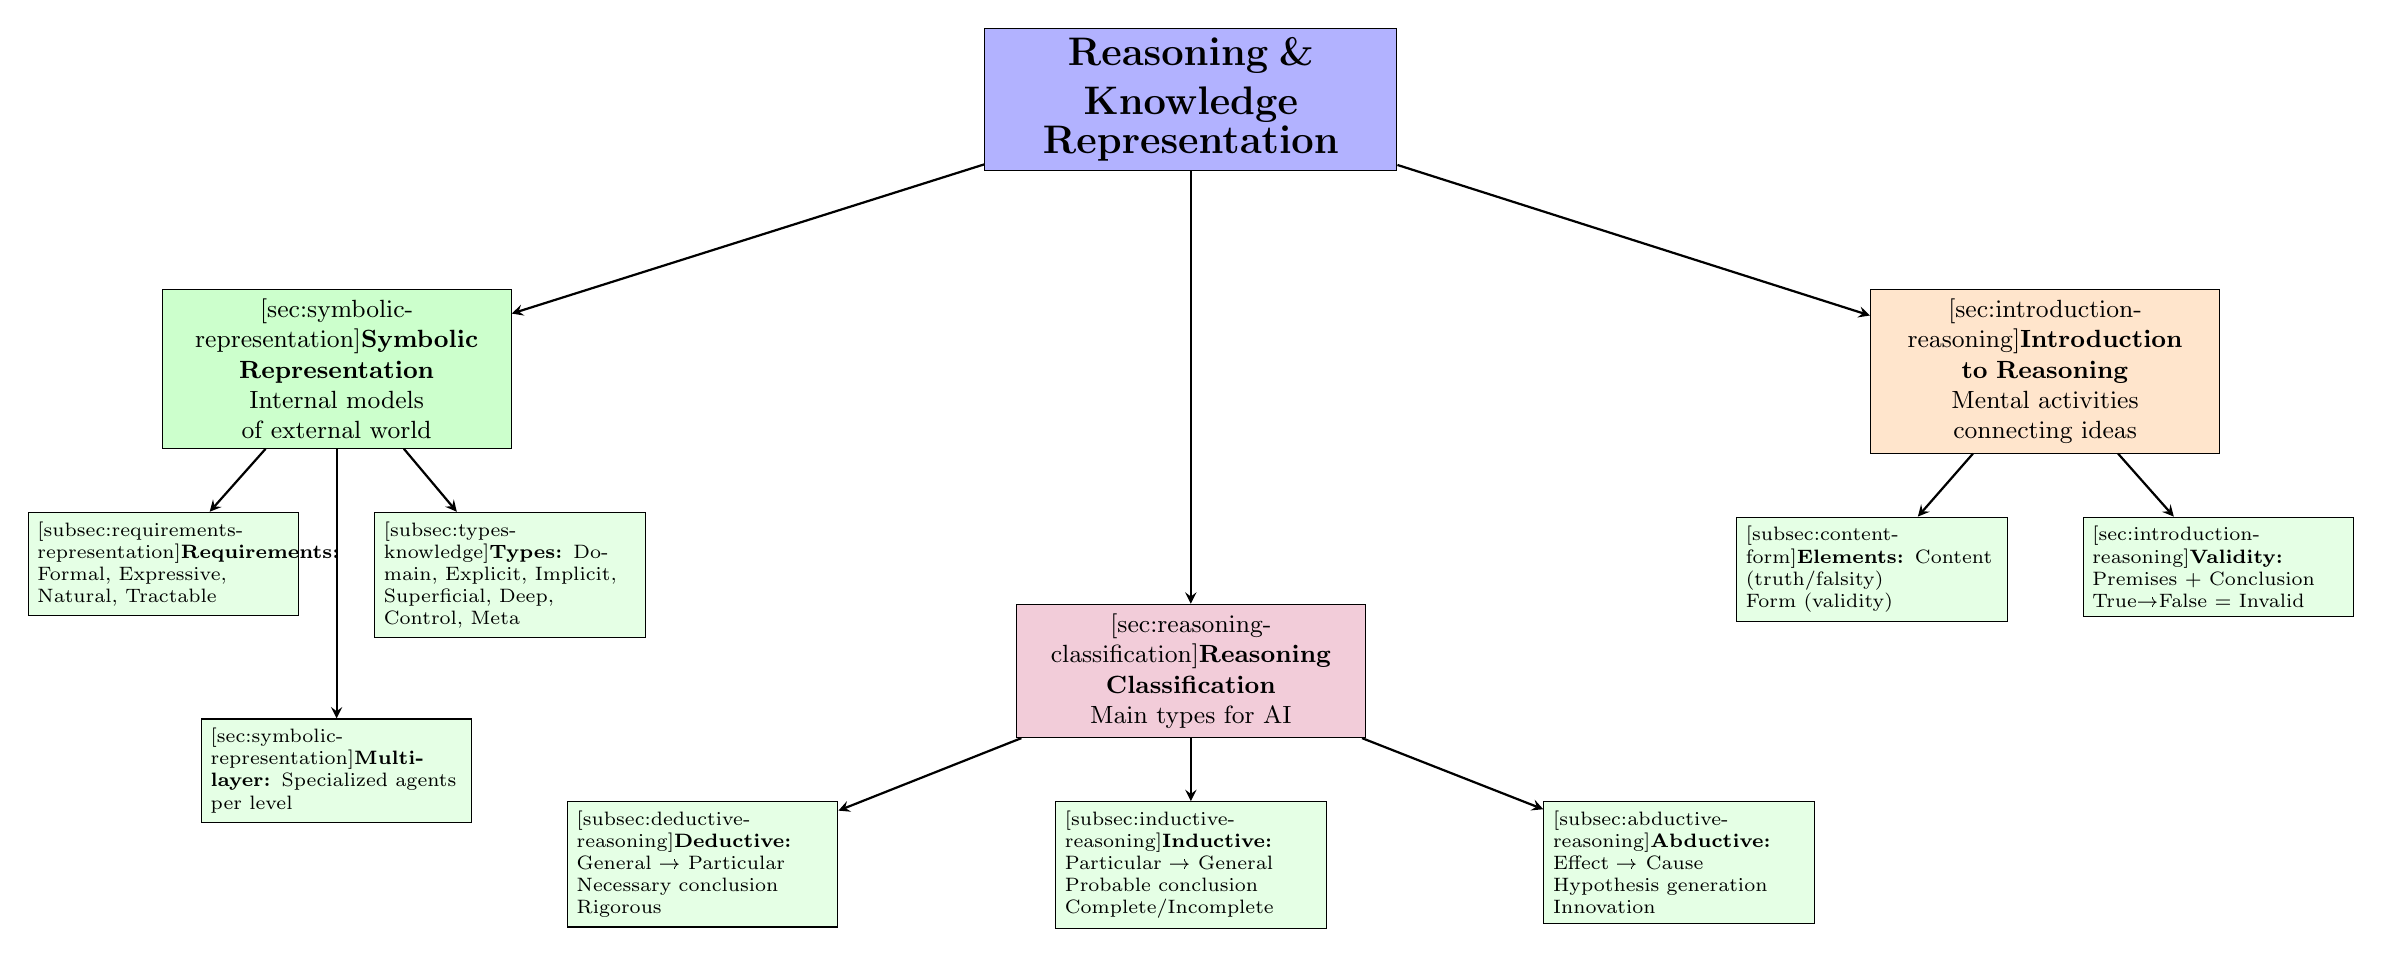
\begin{tikzpicture}[
    node distance=1.5cm and 2cm,
    box/.style={rectangle, draw, fill=blue!10, text width=4.2cm, align=center, minimum height=1cm, font=\small},
    titlebox/.style={rectangle, draw, fill=blue!30, text width=5cm, align=center, minimum height=1.2cm, font=\bfseries},
    smallbox/.style={rectangle, draw, fill=green!10, text width=3.2cm, align=left, minimum height=0.8cm, font=\scriptsize},
    arrow/.style={->, >=stealth, thick}
]

% Main title
\node[titlebox] (main) at (0,0) {\Large Reasoning \& Knowledge\\Representation};

% Symbolic Representation section
\node[box, fill=green!20, below left=of main, xshift=-4cm] (sr) {\hyperref[sec:symbolic-representation]{\textbf{Symbolic Representation}}\\Internal models of external world};
\node[smallbox, below=0.8cm of sr, xshift=-2.2cm] (sr-req) {\hyperref[subsec:requirements-representation]{\textbf{Requirements:}} Formal, Expressive,\\Natural, Tractable};
\node[smallbox, below=0.8cm of sr, xshift=2.2cm] (sr-types) {\hyperref[subsec:types-knowledge]{\textbf{Types:}} Domain, Explicit, Implicit,\\Superficial, Deep,\\Control, Meta};
\node[smallbox, below=0.8cm of sr-req, yshift=-0.5cm, xshift=2.2cm] (sr-multi) {\hyperref[sec:symbolic-representation]{\textbf{Multi-layer:}} Specialized agents\\per level};

% Introduction to Reasoning section
\node[box, fill=orange!20, below right=of main, xshift=4cm] (ir) {\hyperref[sec:introduction-reasoning]{\textbf{Introduction to Reasoning}}\\Mental activities connecting ideas};
\node[smallbox, below=0.8cm of ir, xshift=-2.2cm] (ir-elem) {\hyperref[subsec:content-form]{\textbf{Elements:}} Content (truth/falsity)\\Form (validity)};
\node[smallbox, below=0.8cm of ir, xshift=2.2cm] (ir-valid) {\hyperref[sec:introduction-reasoning]{\textbf{Validity:}} Premises + Conclusion\\True→False = Invalid};

% Reasoning Classification section
\node[box, fill=purple!20, below=5.5cm of main] (rc) {\hyperref[sec:reasoning-classification]{\textbf{Reasoning Classification}}\\Main types for AI};

\node[smallbox, below=0.8cm of rc, xshift=-6.2cm] (ded) {\hyperref[subsec:deductive-reasoning]{\textbf{Deductive:}} General → Particular\\Necessary conclusion\\Rigorous};
\node[smallbox, below=0.8cm of rc, xshift=0cm] (ind) {\hyperref[subsec:inductive-reasoning]{\textbf{Inductive:}} Particular → General\\Probable conclusion\\Complete/Incomplete};
\node[smallbox, below=0.8cm of rc, xshift=6.2cm] (abd) {\hyperref[subsec:abductive-reasoning]{\textbf{Abductive:}} Effect → Cause\\Hypothesis generation\\Innovation};

% Arrows
\draw[arrow] (main) -- (sr);
\draw[arrow] (main) -- (ir);
\draw[arrow] (main) -- (rc);

\draw[arrow] (sr) -- (sr-req);
\draw[arrow] (sr) -- (sr-types);
\draw[arrow] (sr) -- (sr-multi);

\draw[arrow] (ir) -- (ir-elem);
\draw[arrow] (ir) -- (ir-valid);

\draw[arrow] (rc) -- (ded);
\draw[arrow] (rc) -- (ind);
\draw[arrow] (rc) -- (abd);

\end{tikzpicture}
}
\caption{Conceptual map of the Reasoning and Planning course - Lecture 002}
\end{figure}



% Lecture 003
\section*{Lecture 003}
\section{Introduction to Logic}
\label{sec:introduction-logic}

Logic is key for representing human thinking and building systems that emulate thought processes. It's a tool for explaining knowledge based on reasoning elements: categories, definitions, judgments, and propositions. From Aristotle to today, logic has evolved into a powerful tool for modeling behavior in AI.

Logic is a \textbf{formal science} (not empirical). \textbf{Formal sciences} like logic and mathematics work with abstract structures, symbols, and inference rules through \textbf{deductive} reasoning—starting from axioms and deriving conclusions via formal rules, no empirical observation needed. \textbf{Empirical sciences} like physics and biology observe the world and test hypotheses through experimentation using \textbf{inductive} reasoning. Logic studies the \textbf{structure of reasoning itself}, focusing on abstract relationships and formal rules, regardless of whether statements are actually true in reality.

Logic enables \textbf{formal representation of relationships} between objects and their properties, useful for emulating human thinking, modeling AI behavior, and identifying valid reasoning patterns.

\textbf{Aristotle} is considered the father of logic. He developed the \textbf{syllogism}—two premises leading to one conclusion. Example: "All humans are mortal. Socrates is a human. Therefore, Socrates is mortal."


\subsection{Types of Logic}
\label{subsec:types-logic}

There are several types of logic, all focused on understanding reasoning and determining if it's correct or incorrect. They study statements beyond natural language, extending to mathematics and computer science with very different structures.

\begin{itemize}
    \item \textbf{Propositional logic}: Uses propositions (statements that can be true or false) connected with logical operators ($\land$ [and], $\lor$ [or], $\neg$ [not]) and rules with implication ($\rightarrow$). Uses inference mechanisms like modus ponens and modus tollens.
    
    \item \textbf{Predicate logic}: Extends propositional logic by adding quantifiers:
    \begin{itemize}
        \item $\forall$ (for all)
        \item $\exists$ (there exists)
    \end{itemize}
    Uses traditional inference mechanisms (modus ponens, modus tollens). Example: PROLOG programming language.
    
    \item \textbf{First-order logic}: Formal system for studying inference in first-order languages. Uses quantifiers over individual variables with predicates and functions. Establishes objects and relationships between them. Foundation of computational logic.
    
    \item \textbf{Formal logic} (classical/Aristotelian): Studies propositions and arguments from a structural perspective. Focuses on argument structure, not content truth/falsity. Includes:
    \begin{itemize}
        \item \textbf{Deductive logic}
        \item \textbf{Inductive logic}
    \end{itemize}
    
    \item \textbf{Symbolic/Mathematical logic}: Uses symbols to build a new language for expressing arguments. Translates human thought to mathematical language, converting abstract thinking into formal structures. Used in mathematics to prove theorems.
    
    \item \textbf{Class logic}: Based on set theory. Analyzes logical propositions about membership (or non-membership) of an element to a class (set of elements sharing a characteristic).
    
    \item \textbf{Material logic}: Studied from epistemology. Includes uncertainty—conclusions involve some degree of doubt. Proves validity of reasoning based on reality.
    
    \item \textbf{Natural logic}: Related to empiricism, learning through trial and error. Innate reason that prevents humans from repeating the same mistake.
    
    \item \textbf{Scientific logic}: Extends natural logic by including reason, creating frameworks for everything that exists. Based on finding reasons or justifications for why facts occur.
    
    \item \textbf{Informal logic}: Focuses on language and meaning of semantic constructions and arguments. Differs from formal logic by focusing on sentence content rather than structure.
    
    \item \textbf{Modern logic}: Born in the 19th century, differs from classical logic by including mathematical and symbolic elements, theorems that replace formal logic limitations. Includes:
    \begin{itemize}
        \item \textbf{Modal logic}: Adds modal operators to determine if statements are true/false. Considers expressions like "always", "very likely", "sometimes", "maybe".
        \item \textbf{Mathematical logic}
        \item \textbf{Trivalent logic}
    \end{itemize}
    
    \item \textbf{Computational logic}: Derives from symbolic/mathematical logic (first-order) and applies to computer science. Enables working with programming languages for specific verification tasks.
\end{itemize}

The logics most relevant to artificial intelligence (which will be covered in detail later) are: mathematical logic, description logic (ALC), higher-order logic, multivalued logic, and fuzzy logic.


\section{Propositional Logic}
\label{sec:propositional-logic}

Propositional logic (also called sentential logic or statement logic) is the most basic form of logic. It deals with simple propositions that can be true or false, and how they can be combined using logical connectives.

\subsection{Basic Concepts}
\label{subsec:propositional-basics}

A \textbf{proposition} is any statement or expression that has meaning and of which we can say whether it is false (F/0) or true (V/1). Propositions can be linked together using logical connectives to form structures with precise meaning.

\textbf{Not propositions}: imperative sentences (commands like "read this"), exclamatory and interrogative sentences (questions like "what's your name?"), and instructions (like "go back").

Propositions are usually represented with lowercase letters, e.g., $p$, $q$, $r$. By relating propositions, it's possible to obtain other propositions. All logical reasoning must necessarily start from an adequate connection of some elementary propositions.

Propositions can be classified into:

\begin{itemize}
    \item \textbf{Tautologies}: A compound proposition is a tautology if it's true for all assignments of truth values to its component propositions. Its truth value doesn't depend on the truth values of the propositions that form it, but on the way syntactic relationships are established between propositions.
    
    \item \textbf{Contradictions}: Propositions that, in all possible cases of their truth table, are always false. Their false value doesn't depend on the truth values of the propositions that form them, but on the way syntactic relationships are established between propositions.
    
    \item \textbf{Contingencies, fallacies, or inconsistencies}: Also called "truth of fact," these are propositions that can be true or false, combining tautology and contradiction, depending on the values of the propositions that compose them.
\end{itemize}

A \textbf{truth table} is a table that shows all possible combinations of truth values for the component propositions and the resulting truth value of the compound proposition.

\subsection{Logical Connectives}
\label{subsec:logical-connectives}

The main logical connectives and their truth tables are:

\begin{itemize}
    \item \textbf{Negation} ($\neg$): Denies a proposition. The negation of $p$ is true when $p$ is false, and false when $p$ is true.
    
    \begin{table}[H]
    \centering
    \caption{Truth Table for Negation}
    \label{tab:negation}
    \begin{tabular}{c|c}
    \toprule
    $p$ & $\neg p$ \\
    \midrule
    1 & 0 \\
    0 & 1 \\
    \bottomrule
    \end{tabular}
    \end{table}
    
    \item \textbf{Conjunction} ($\land$): "And". The conjunction $p \land q$ is true only when both $p$ and $q$ are true.
    
    \begin{table}[H]
    \centering
    \caption{Truth Table for Conjunction}
    \label{tab:conjunction}
    \begin{tabular}{cc|c}
    \toprule
    $p$ & $q$ & $p \land q$ \\
    \midrule
    1 & 1 & 1 \\
    1 & 0 & 0 \\
    0 & 1 & 0 \\
    0 & 0 & 0 \\
    \bottomrule
    \end{tabular}
    \end{table}
    
    \item \textbf{Non-exclusive disjunction} ($\lor$): "Or" (inclusive). The disjunction $p \lor q$ is true when at least one of $p$ or $q$ is true (or both).
    
    \begin{table}[H]
    \centering
    \caption{Truth Table for Non-exclusive Disjunction}
    \label{tab:disjunction}
    \begin{tabular}{cc|c}
    \toprule
    $p$ & $q$ & $p \lor q$ \\
    \midrule
    1 & 1 & 1 \\
    1 & 0 & 1 \\
    0 & 1 & 1 \\
    0 & 0 & 0 \\
    \bottomrule
    \end{tabular}
    \end{table}
    
    \item \textbf{Exclusive disjunction} ($\oplus$ or $\veebar$): "Either...or" (exclusive). The exclusive disjunction $p \oplus q$ is true when exactly one of $p$ or $q$ is true, but not both.
    
    \begin{table}[H]
    \centering
    \caption{Truth Table for Exclusive Disjunction}
    \label{tab:exclusive-disjunction}
    \begin{tabular}{cc|c}
    \toprule
    $p$ & $q$ & $p \oplus q$ \\
    \midrule
    1 & 1 & 0 \\
    1 & 0 & 1 \\
    0 & 1 & 1 \\
    0 & 0 & 0 \\
    \bottomrule
    \end{tabular}
    \end{table}
    
    \item \textbf{Conditional} ($\rightarrow$): "If...then". The conditional $p \rightarrow q$ is false only when $p$ is true and $q$ is false. Otherwise, it's true.
    
    \begin{table}[H]
    \centering
    \caption{Truth Table for Conditional}
    \label{tab:conditional}
    \begin{tabular}{cc|c}
    \toprule
    $p$ & $q$ & $p \rightarrow q$ \\
    \midrule
    1 & 1 & 1 \\
    1 & 0 & 0 \\
    0 & 1 & 1 \\
    0 & 0 & 1 \\
    \bottomrule
    \end{tabular}
    \end{table}
    
    \item \textbf{Biconditional} ($\leftrightarrow$): "If and only if". The biconditional $p \leftrightarrow q$ is true when both $p$ and $q$ have the same truth value (both true or both false).
    
    \begin{table}[H]
    \centering
    \caption{Truth Table for Biconditional}
    \label{tab:biconditional}
    \begin{tabular}{cc|c}
    \toprule
    $p$ & $q$ & $p \leftrightarrow q$ \\
    \midrule
    1 & 1 & 1 \\
    1 & 0 & 0 \\
    0 & 1 & 0 \\
    0 & 0 & 1 \\
    \bottomrule
    \end{tabular}
    \end{table}
\end{itemize}

Key concepts for relationships between propositions:

\begin{itemize}
    \item \textbf{Logical implication}: Any conditional that is a tautology. When a conditional statement ($p \rightarrow q$) is always true regardless of the truth values of its component propositions, it represents a logical implication.
    
    \textit{Example}: $(p \land q) \rightarrow p$ (if both $p$ and $q$ are true, then $p$ is true). This is a logical implication because the conditional is always true, as shown in Table~\ref{tab:logical-implication}:
    
    \begin{table}[H]
    \centering
    \caption{Truth Table for Logical Implication: $(p \land q) \rightarrow p$}
    \label{tab:logical-implication}
    \begin{tabular}{ccc|c}
    \toprule
    $p$ & $q$ & $p \land q$ & $(p \land q) \rightarrow p$ \\
    \midrule
    1 & 1 & 1 & \textcolor{green}{1} \\
    1 & 0 & 0 & \textcolor{green}{1} \\
    0 & 1 & 0 & \textcolor{green}{1} \\
    0 & 0 & 0 & \textcolor{green}{1} \\
    \bottomrule
    \end{tabular}
    \end{table}
    
    \item \textbf{Logical equivalence}: Any biconditional that is a tautology. When a biconditional statement ($p \leftrightarrow q$) is always true regardless of the truth values of its component propositions, the propositions are logically equivalent.
    
    \textit{Example}: $\neg(\neg p) \leftrightarrow p$ (double negation). This is a logical equivalence because the biconditional is always true, as shown in Table~\ref{tab:logical-equivalence}:
    
    \begin{table}[H]
    \centering
    \caption{Truth Table for Logical Equivalence: $\neg(\neg p) \leftrightarrow p$}
    \label{tab:logical-equivalence}
    \begin{tabular}{cc|c}
    \toprule
    $p$ & $\neg(\neg p)$ & $\neg(\neg p) \leftrightarrow p$ \\
    \midrule
    1 & 1 & \textcolor{green}{1} \\
    0 & 0 & \textcolor{green}{1} \\
    \bottomrule
    \end{tabular}
    \end{table}
\end{itemize}

\subsubsection{Example: Robbery Investigation}
\label{subsubsec:robbery-example}

\textbf{Problem statement}: A robbery has occurred and it's known that the perpetrators fled in a car. Three known criminals (Par, Qun, and Rag) are interrogated. The police obtain the following information:

\begin{enumerate}
    \item Par, Qun, and Rag are the only possible culprits
    \item Rag never does a job without Par as an accomplice (doesn't exclude others)
    \item Qun doesn't know how to drive
\end{enumerate}

How can we identify the guilty persons?

\textbf{Solution using Truth Tables}:

\textit{Step 1: Define propositions}

Let's represent each suspect with a proposition:
\begin{itemize}
    \item $P$: Par participated in the robbery
    \item $Q$: Qun participated in the robbery
    \item $R$: Rag participated in the robbery
\end{itemize}

\textit{Step 2: Translate information into logical statements}

\begin{enumerate}
    \item At least one person participated (there was a robbery): $P \lor Q \lor R$
    \item Rag never works without Par: $R \rightarrow P$
    \item Qun doesn't know how to drive, someone must drive: $Q \rightarrow (P \lor R)$
\end{enumerate}

Let $C$ represent all constraints combined:
$$C = (P \lor Q \lor R) \land (R \rightarrow P) \land (Q \rightarrow (P \lor R))$$

\textit{Step 3: Build the truth table for all combinations}

\begin{table}[H]
\centering
\caption{Truth Table for Constraints}
\label{tab:robbery-truth-table}
\begin{tabular}{ccc|ccc|c}
\toprule
$P$ & $Q$ & $R$ & $P \lor Q \lor R$ & $R \rightarrow P$ & $Q \rightarrow (P \lor R)$ & $C$ \\
\midrule
0 & 0 & 0 & 0 & 1 & 1 & 0 \\
\rowcolor{gray!30}
0 & 0 & 1 & 1 & 0 & 1 & 0 \\
\rowcolor{gray!30}
0 & 1 & 0 & 1 & 1 & 0 & 0 \\
\rowcolor{gray!30}
0 & 1 & 1 & 1 & 0 & 1 & 0 \\
1 & 0 & 0 & 1 & 1 & 1 & \textcolor{green}{1} \\
1 & 0 & 1 & 1 & 1 & 1 & \textcolor{green}{1} \\
1 & 1 & 0 & 1 & 1 & 1 & \textcolor{green}{1} \\
1 & 1 & 1 & 1 & 1 & 1 & \textcolor{green}{1} \\
\bottomrule
\end{tabular}
\end{table}

Notice that $C = 1$ (constraints are satisfied) only when $P = 1$ in rows 5, 6, 7, and 8.

\textit{Step 4: Check which suspects must be guilty using logical implication}

To determine who must be guilty, we check if $C \rightarrow X$ is a tautology for each suspect $X$:

\begin{table}[H]
\centering
\caption{Testing Logical Implications}
\label{tab:robbery-implications}
\begin{tabular}{ccc|c|ccc}
\toprule
$P$ & $Q$ & $R$ & $C$ & $C \rightarrow P$ & $C \rightarrow Q$ & $C \rightarrow R$ \\
\midrule
0 & 0 & 0 & 0 & 1 & 1 & 1 \\
0 & 0 & 1 & 0 & 1 & 1 & 1 \\
0 & 1 & 0 & 0 & 1 & 1 & 1 \\
0 & 1 & 1 & 0 & 1 & 1 & 1 \\
1 & 0 & 0 & 1 & \textcolor{green}{1} & \textcolor{red}{0} & \textcolor{red}{0} \\
1 & 0 & 1 & 1 & \textcolor{green}{1} & \textcolor{red}{0} & \textcolor{green}{1} \\
1 & 1 & 0 & 1 & \textcolor{green}{1} & \textcolor{green}{1} & \textcolor{red}{0} \\
1 & 1 & 1 & 1 & \textcolor{green}{1} & \textcolor{green}{1} & \textcolor{green}{1} \\
\bottomrule
\end{tabular}
\end{table}

\textit{Step 5: Conclusion}

\begin{itemize}
    \item $C \rightarrow P$ is a \textbf{tautology} (all values are 1) $\rightarrow$ \textbf{Par is definitely guilty}
    \item $C \rightarrow Q$ is \textbf{not} a tautology (contains 0) $\rightarrow$ Qun may or may not be guilty
    \item $C \rightarrow R$ is \textbf{not} a tautology (contains 0) $\rightarrow$ Rag may or may not be guilty
\end{itemize}

\textbf{Answer}: \textbf{Par is definitely guilty}. We cannot determine with certainty whether Qun and/or Rag participated. Since $C \rightarrow P$ is a tautology, $P$ is a \textbf{logical consequence} of the constraints.

\textbf{Alternative Solution using Logical Reasoning}:

We can also solve this by analyzing scenarios:

Notice that in \textbf{all valid scenarios (where $C = 1$), Par must be true}:
\begin{itemize}
    \item Par alone: $P \land \neg Q \land \neg R$ (row 5)
    \item Par and Rag: $P \land \neg Q \land R$ (row 6)
    \item Par and Qun: $P \land Q \land \neg R$ (row 7)
    \item All three: $P \land Q \land R$ (row 8)
\end{itemize}

We can prove Par's guilt by contradiction:
\begin{itemize}
    \item Suppose $\neg P$ (Par didn't participate)
    \item From $R \rightarrow P$, by contrapositive: $\neg P \rightarrow \neg R$, so Rag didn't participate
    \item If only Qun participated ($Q \land \neg P \land \neg R$), no one could drive $\rightarrow$ impossible
    \item Therefore, $P$ must be true
\end{itemize}

\subsection{Propositional Logic - Detailed Concept Map}
\label{subsec:propositional-logic-conceptmap}

\begin{figure}[H]
\centering
\resizebox{1\textwidth}{!}{
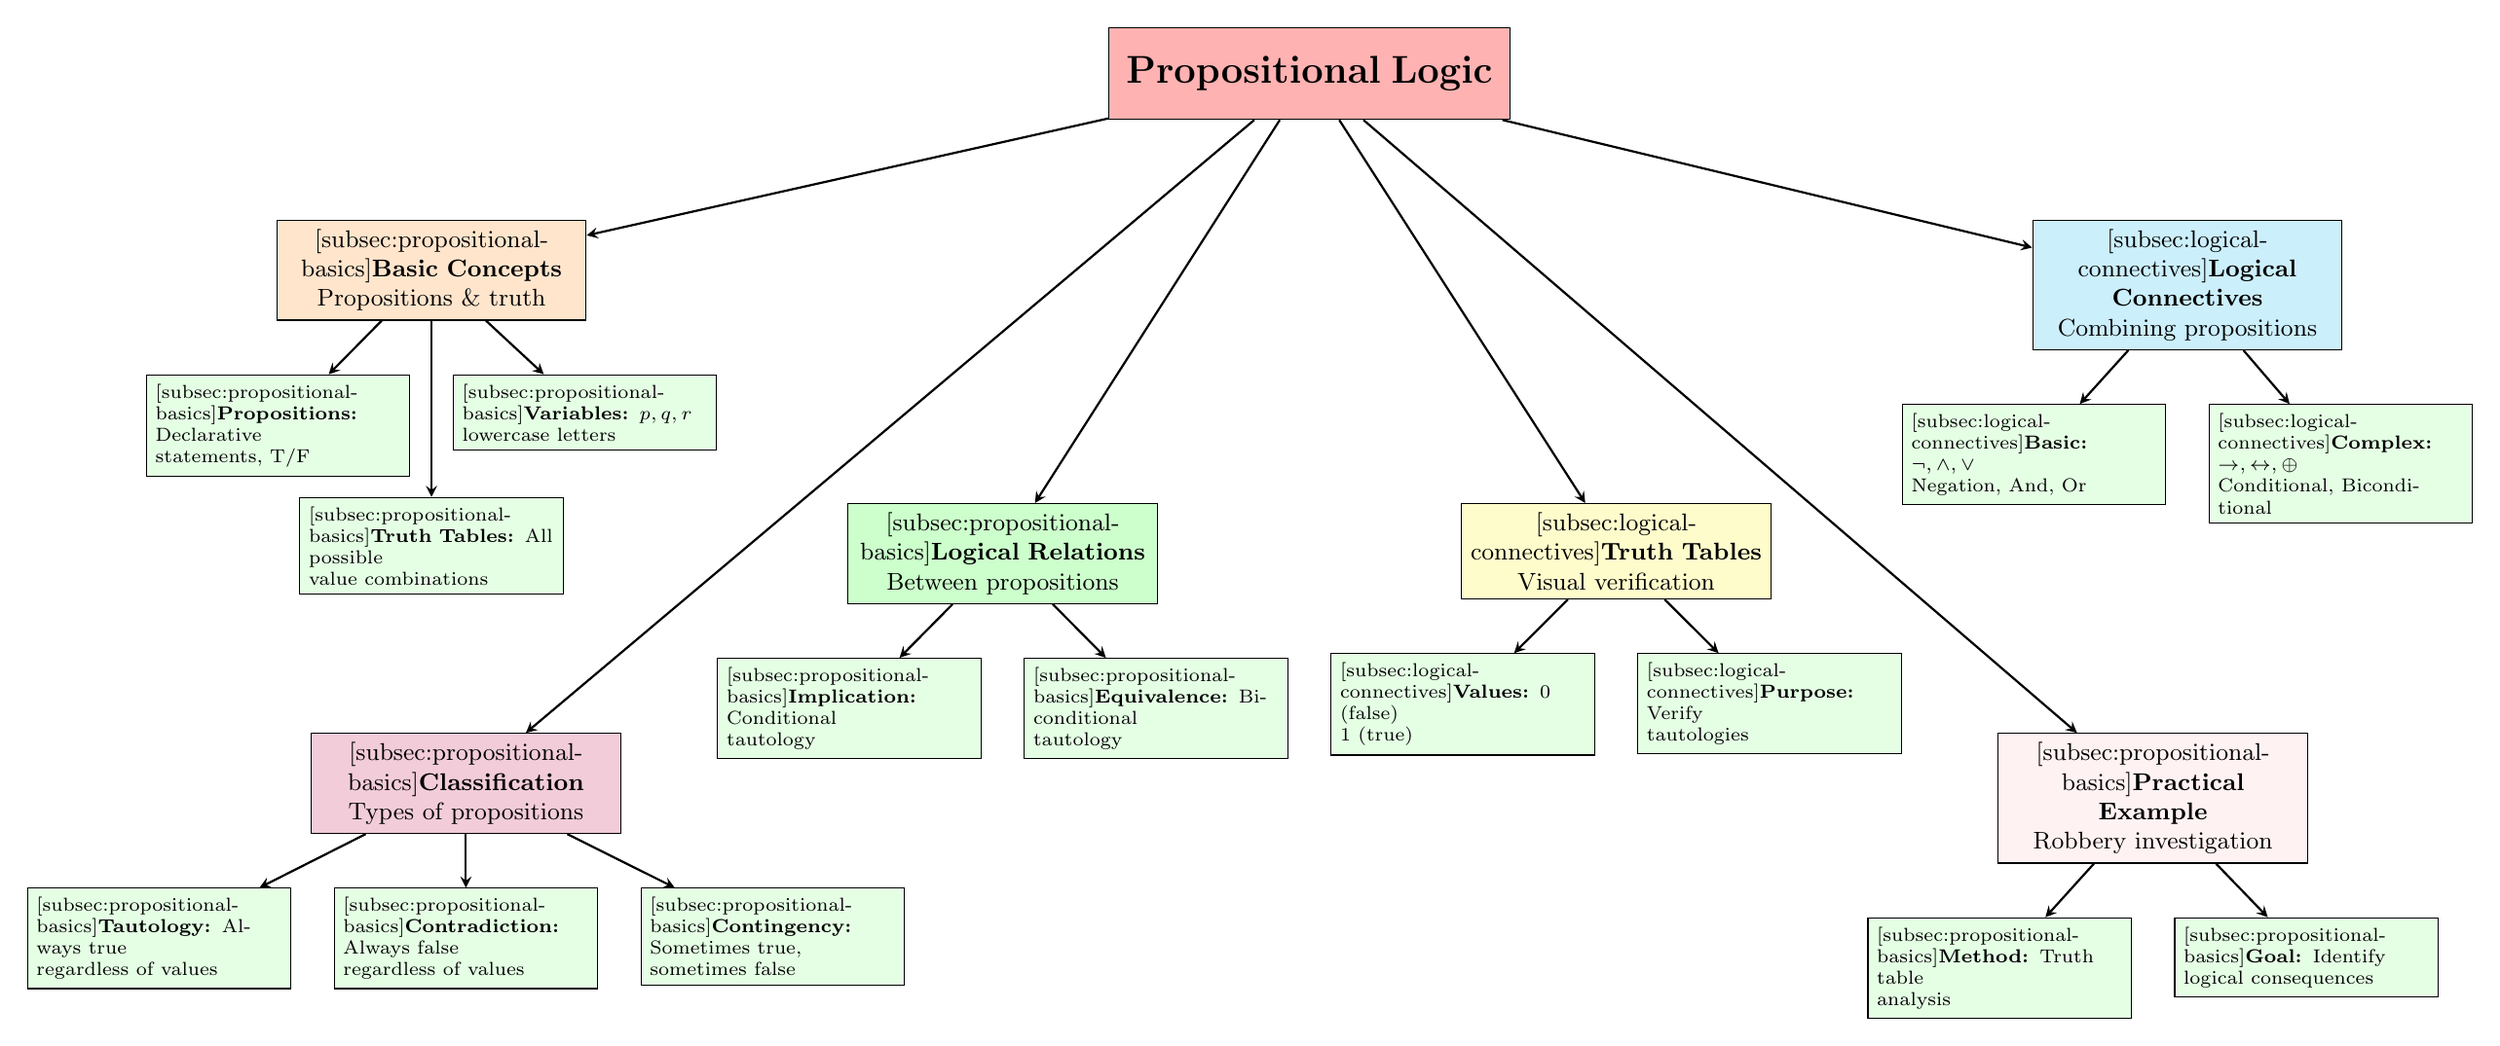
\begin{tikzpicture}[
    node distance=1.3cm and 1.8cm,
    box/.style={rectangle, draw, fill=blue!10, text width=3.8cm, align=center, minimum height=1cm, font=\small},
    titlebox/.style={rectangle, draw, fill=red!30, text width=5cm, align=center, minimum height=1.2cm, font=\bfseries},
    smallbox/.style={rectangle, draw, fill=green!10, text width=3.2cm, align=left, minimum height=0.8cm, font=\scriptsize},
    arrow/.style={->, >=stealth, thick}
]

% Main title
\node[titlebox] (main) at (0,0) {\Large Propositional Logic};

% Row 1: Basic Concepts
\node[box, fill=orange!20, below left=of main, xshift=-5cm, ] (basics) {\hyperref[subsec:propositional-basics]{\textbf{Basic Concepts}}\\Propositions \& truth};
\node[smallbox, below=0.7cm of basics, xshift=-2cm] (basics-1) {\hyperref[subsec:propositional-basics]{\textbf{Propositions:}} Declarative\\statements, T/F};
\node[smallbox, below=0.7cm of basics, xshift=2cm] (basics-2) {\hyperref[subsec:propositional-basics]{\textbf{Variables:}} $p, q, r$\\lowercase letters};
\node[smallbox, below=2.3cm of basics] (basics-3) {\hyperref[subsec:propositional-basics]{\textbf{Truth Tables:}} All possible\\value combinations};

% Row 1: Logical Connectives
\node[box, fill=cyan!20, below right=of main, xshift=5cm, ] (connectives) {\hyperref[subsec:logical-connectives]{\textbf{Logical Connectives}}\\Combining propositions};
\node[smallbox, below=0.7cm of connectives, xshift=-2cm] (conn-1) {\hyperref[subsec:logical-connectives]{\textbf{Basic:}} $\neg, \land, \lor$\\Negation, And, Or};
\node[smallbox, below=0.7cm of connectives, xshift=2cm] (conn-2) {\hyperref[subsec:logical-connectives]{\textbf{Complex:}} $\rightarrow, \leftrightarrow, \oplus$\\Conditional, Biconditional};

% Row 2: Classification
\node[box, fill=purple!20, below=8cm of main, xshift=-11cm] (class) {\hyperref[subsec:propositional-basics]{\textbf{Classification}}\\Types of propositions};
\node[smallbox, below=0.7cm of class, xshift=-4cm] (class-1) {\hyperref[subsec:propositional-basics]{\textbf{Tautology:}} Always true\\regardless of values};
\node[smallbox, below=0.7cm of class] (class-2) {\hyperref[subsec:propositional-basics]{\textbf{Contradiction:}} Always false\\regardless of values};
\node[smallbox, below=0.7cm of class, xshift=4cm] (class-3) {\hyperref[subsec:propositional-basics]{\textbf{Contingency:}} Sometimes true,\\sometimes false};

% Row 2: Logical Relations
\node[box, fill=green!20, below=5cm of main, xshift=-4cm] (relations) {\hyperref[subsec:propositional-basics]{\textbf{Logical Relations}}\\Between propositions};
\node[smallbox, below=0.7cm of relations, xshift=-2cm] (rel-1) {\hyperref[subsec:propositional-basics]{\textbf{Implication:}} Conditional\\tautology};
\node[smallbox, below=0.7cm of relations, xshift=2cm] (rel-2) {\hyperref[subsec:propositional-basics]{\textbf{Equivalence:}} Biconditional\\tautology};

% Row 2: Truth Tables
\node[box, fill=yellow!20, below=5cm of main, xshift=4cm] (tables) {\hyperref[subsec:logical-connectives]{\textbf{Truth Tables}}\\Visual verification};
\node[smallbox, below=0.7cm of tables, xshift=-2cm] (tab-1) {\hyperref[subsec:logical-connectives]{\textbf{Values:}} 0 (false)\\1 (true)};
\node[smallbox, below=0.7cm of tables, xshift=2cm] (tab-2) {\hyperref[subsec:logical-connectives]{\textbf{Purpose:}} Verify\\tautologies};

% Row 2: Examples
\node[box, fill=pink!20, below=8cm of main, xshift=11cm] (examples) {\hyperref[subsec:propositional-basics]{\textbf{Practical Example}}\\Robbery investigation};
\node[smallbox, below=0.7cm of examples, xshift=-2cm] (ex-1) {\hyperref[subsec:propositional-basics]{\textbf{Method:}} Truth table\\analysis};
\node[smallbox, below=0.7cm of examples, xshift=2cm] (ex-2) {\hyperref[subsec:propositional-basics]{\textbf{Goal:}} Identify\\logical consequences};

% Arrows from main
\draw[arrow] (main) -- (basics);
\draw[arrow] (main) -- (connectives);
\draw[arrow] (main) -- (class);
\draw[arrow] (main) -- (relations);
\draw[arrow] (main) -- (tables);
\draw[arrow] (main) -- (examples);

% Arrows to sub-boxes
\draw[arrow] (basics) -- (basics-1);
\draw[arrow] (basics) -- (basics-2);
\draw[arrow] (basics) -- (basics-3);
\draw[arrow] (connectives) -- (conn-1);
\draw[arrow] (connectives) -- (conn-2);
\draw[arrow] (class) -- (class-1);
\draw[arrow] (class) -- (class-2);
\draw[arrow] (class) -- (class-3);
\draw[arrow] (relations) -- (rel-1);
\draw[arrow] (relations) -- (rel-2);
\draw[arrow] (tables) -- (tab-1);
\draw[arrow] (tables) -- (tab-2);
\draw[arrow] (examples) -- (ex-1);
\draw[arrow] (examples) -- (ex-2);

\end{tikzpicture}
}
\caption{Detailed conceptual map of Propositional Logic}
\label{fig:propositional-logic-conceptmap}
\end{figure}


\section{First-Order Logic}
\label{sec:first-order-logic}

First-order logic (also called predicate logic) extends propositional logic by allowing quantification over individuals and the use of predicates, functions, and variables. It's more expressive than propositional logic and can represent relationships between objects and properties.

\textbf{Key components}:
\begin{itemize}
    \item \textbf{Constants}: Specific individuals (e.g., $john$, $mary$)
    \item \textbf{Variables}: Placeholders for individuals (e.g., $x$, $y$, $z$)
    \item \textbf{Predicates}: Properties or relations (e.g., $Student(x)$, $Loves(x,y)$)
    \item \textbf{Functions}: Map individuals to individuals (e.g., $mother(x)$)
    \item \textbf{Quantifiers}:
    \begin{itemize}
        \item $\forall x$ (universal): "For all $x$"
        \item $\exists x$ (existential): "There exists an $x$"
    \end{itemize}
\end{itemize}

\textbf{Example}: "All humans are mortal" can be expressed as:
$$\forall x \ (Human(x) \rightarrow Mortal(x))$$

This reads: "For all $x$, if $x$ is a human, then $x$ is mortal."

Another example: "Some students study" can be expressed as:
$$\exists x \ (Student(x) \land Studies(x))$$

This reads: "There exists an $x$ such that $x$ is a student and $x$ studies."

\textbf{More examples}:

"Every mother loves her children" (using a binary relation):
$$\forall x \forall y \ (Mother(x,y) \rightarrow Loves(x,y))$$

This reads: "For all $x$ and $y$, if $x$ is the mother of $y$, then $x$ loves $y$."

"All students have at least one teacher":
$$\forall x \ (Student(x) \rightarrow \exists y \ (Teacher(y) \land Teaches(y,x)))$$

This reads: "For all $x$, if $x$ is a student, then there exists a $y$ such that $y$ is a teacher and $y$ teaches $x$."

"Nobody loves everyone" (combining negation and quantifiers):
$$\neg \exists x \forall y \ Loves(x,y)$$

This reads: "There does not exist an $x$ such that for all $y$, $x$ loves $y$." Or equivalently: "For all $x$, there exists a $y$ such that $x$ does not love $y$."

"Everyone has a mother" (using a function):
$$\forall x \exists y \ (Mother(y,x))$$

This reads: "For all $x$, there exists a $y$ such that $y$ is the mother of $x$." Alternatively, using a function: $\forall x \ (Mother(mother(x),x))$ where $mother(x)$ is a function that returns the mother of $x$.

"All teachers who teach students are professors":
$$\forall x \ (Teacher(x) \land \exists y \ (Student(y) \land Teaches(x,y)) \rightarrow Professor(x))$$

This reads: "For all $x$, if $x$ is a teacher and there exists a $y$ such that $y$ is a student and $x$ teaches $y$, then $x$ is a professor."

First-order logic is the foundation for many advanced logics, including Description Logic ALC, which is a specialized fragment of first-order logic designed for knowledge representation.

\subsection{First-Order Logic - Detailed Concept Map}
\label{subsec:first-order-logic-conceptmap}

\begin{figure}[H]
\centering
\resizebox{1\textwidth}{!}{
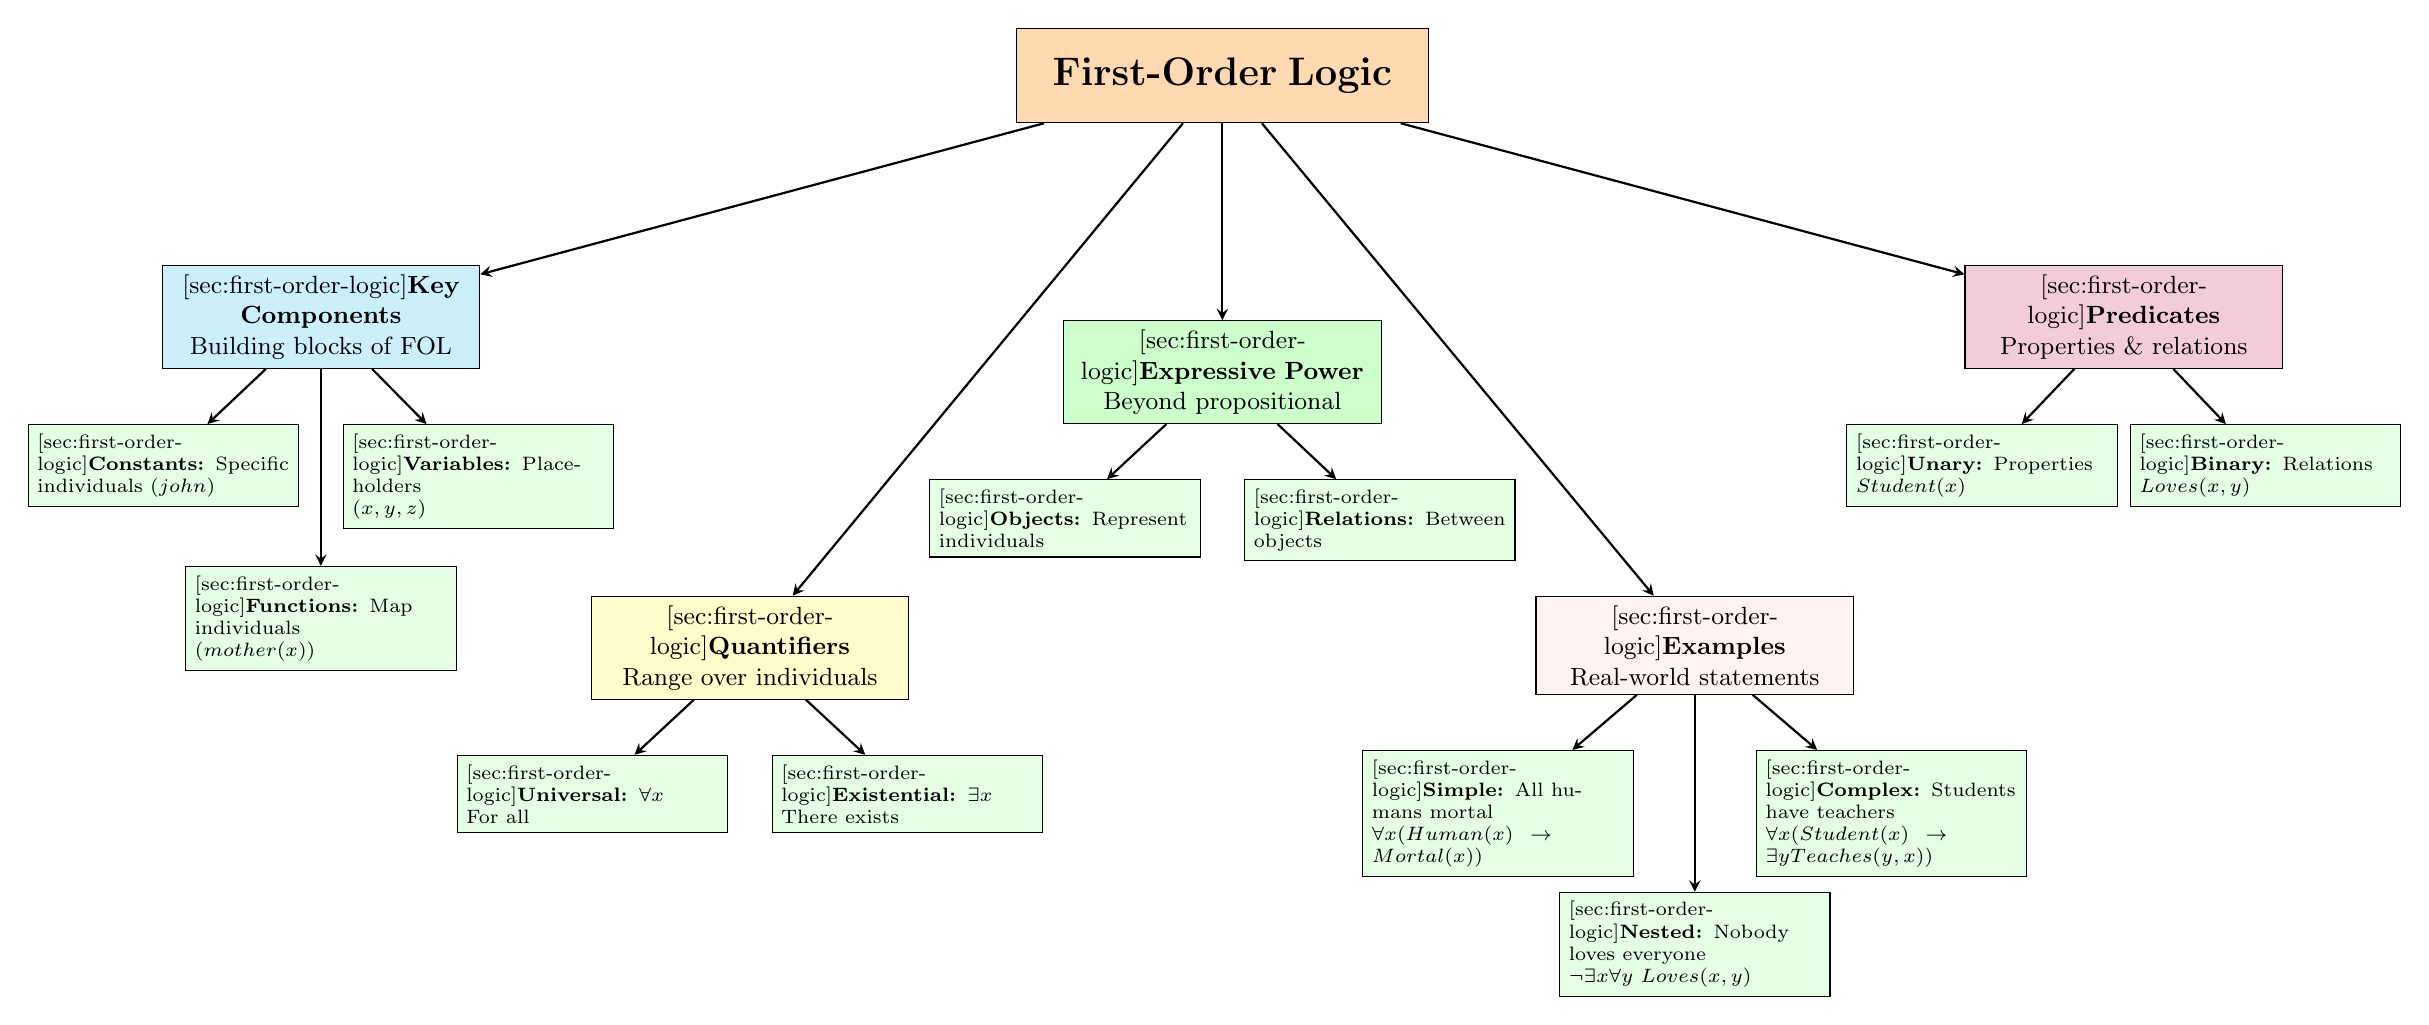
\begin{tikzpicture}[
    node distance=1.3cm and 1.8cm,
    box/.style={rectangle, draw, fill=blue!10, text width=3.8cm, align=center, minimum height=1cm, font=\small},
    titlebox/.style={rectangle, draw, fill=orange!30, text width=5cm, align=center, minimum height=1.2cm, font=\bfseries},
    smallbox/.style={rectangle, draw, fill=green!10, text width=3.2cm, align=left, minimum height=0.8cm, font=\scriptsize},
    arrow/.style={->, >=stealth, thick}
]

% Main title
\node[titlebox] (main) at (0,0) {\Large First-Order Logic};

% Row 1: Components
\node[box, fill=cyan!20, below left=of main, xshift=-5cm, yshift=-0.5cm] (components) {\hyperref[sec:first-order-logic]{\textbf{Key Components}}\\Building blocks of FOL};
\node[smallbox, below=0.7cm of components, xshift=-2cm] (comp-1) {\hyperref[sec:first-order-logic]{\textbf{Constants:}} Specific\\individuals ($john$)};
\node[smallbox, below=0.7cm of components, xshift=2cm] (comp-2) {\hyperref[sec:first-order-logic]{\textbf{Variables:}} Placeholders\\($x, y, z$)};
\node[smallbox, below=2.5cm of components] (comp-3) {\hyperref[sec:first-order-logic]{\textbf{Functions:}} Map individuals\\($mother(x)$)};

% Row 1: Predicates
\node[box, fill=purple!20, below right=of main, xshift=5cm, yshift=-0.5cm] (predicates) {\hyperref[sec:first-order-logic]{\textbf{Predicates}}\\Properties \& relations};
\node[smallbox, below=0.7cm of predicates, xshift=-1.8cm] (pred-1) {\hyperref[sec:first-order-logic]{\textbf{Unary:}} Properties\\$Student(x)$};
\node[smallbox, below=0.7cm of predicates, xshift=1.8cm] (pred-2) {\hyperref[sec:first-order-logic]{\textbf{Binary:}} Relations\\$Loves(x,y)$};

% Row 2: Quantifiers
\node[box, fill=yellow!20, below=6cm of main, xshift=-6cm] (quant) {\hyperref[sec:first-order-logic]{\textbf{Quantifiers}}\\Range over individuals};
\node[smallbox, below=0.7cm of quant, xshift=-2cm] (quant-1) {\hyperref[sec:first-order-logic]{\textbf{Universal:}} $\forall x$\\For all};
\node[smallbox, below=0.7cm of quant, xshift=2cm] (quant-2) {\hyperref[sec:first-order-logic]{\textbf{Existential:}} $\exists x$\\There exists};

% Row 2: Expressive Power
\node[box, fill=green!20, below=2.5cm of main] (power) {\hyperref[sec:first-order-logic]{\textbf{Expressive Power}}\\Beyond propositional};
\node[smallbox, below=0.7cm of power, xshift=-2cm] (pow-1) {\hyperref[sec:first-order-logic]{\textbf{Objects:}} Represent\\individuals};
\node[smallbox, below=0.7cm of power, xshift=2cm] (pow-2) {\hyperref[sec:first-order-logic]{\textbf{Relations:}} Between\\objects};

% Row 2: Examples
\node[box, fill=pink!20, below=6cm of main, xshift=6cm] (examples) {\hyperref[sec:first-order-logic]{\textbf{Examples}}\\Real-world statements};
\node[smallbox, below=0.7cm of examples, xshift=-2.5cm] (ex-1) {\hyperref[sec:first-order-logic]{\textbf{Simple:}} All humans mortal\\$\forall x (Human(x) \rightarrow Mortal(x))$};
\node[smallbox, below=0.7cm of examples, xshift=2.5cm] (ex-2) {\hyperref[sec:first-order-logic]{\textbf{Complex:}} Students have teachers\\$\forall x (Student(x) \rightarrow \exists y Teaches(y,x))$};
\node[smallbox, below=2.5cm of examples] (ex-3) {\hyperref[sec:first-order-logic]{\textbf{Nested:}} Nobody loves everyone\\$\neg \exists x \forall y \ Loves(x,y)$};

% Arrows from main
\draw[arrow] (main) -- (components);
\draw[arrow] (main) -- (predicates);
\draw[arrow] (main) -- (quant);
\draw[arrow] (main) -- (power);
\draw[arrow] (main) -- (examples);

% Arrows to sub-boxes
\draw[arrow] (components) -- (comp-1);
\draw[arrow] (components) -- (comp-2);
\draw[arrow] (components) -- (comp-3);
\draw[arrow] (predicates) -- (pred-1);
\draw[arrow] (predicates) -- (pred-2);
\draw[arrow] (quant) -- (quant-1);
\draw[arrow] (quant) -- (quant-2);
\draw[arrow] (power) -- (pow-1);
\draw[arrow] (power) -- (pow-2);
\draw[arrow] (examples) -- (ex-1);
\draw[arrow] (examples) -- (ex-2);
\draw[arrow] (examples) -- (ex-3);

\end{tikzpicture}
}
\caption{Detailed conceptual map of First-Order Logic}
\label{fig:first-order-logic-conceptmap}
\end{figure}


\section{Description Logic ALC}
\label{sec:description-logic-alc}

Description logics are more than languages for formalizing concepts—they are a set of knowledge representation languages used to represent the terminological knowledge of a specific domain in a structured and formal way, ensuring clear understanding.

They are used to represent \textbf{ontologies} (formalization of a domain) and enable reasoning about them. They introduce new language and semantic elements necessary to formalize:

Description logics are particularly appropriate for the \textbf{semantic web} because they are useful for adding reasoning capabilities to the web. They have a formal syntax that allows describing:
\begin{itemize}
    \item Important concepts of a universe or domain
    \item Relationships that arise or exist between them
    \item Constructors for building new concepts
\end{itemize}

Like all formal logics, they make it possible to reason based on knowledge that has been defined as such. Description logics are \textbf{variants of first-order logic}.


The formal characteristics of description logic include:

\begin{itemize}
    \item \textbf{Ontology modeling}: They model ontologies, provide descriptions to domains, and formalize the elements of a terminology or descriptions of an ontology. The syntax and semantics have no ambiguity, as they are formal.
    
    \item \textbf{Descriptive formalism}: Uses three main components:
    \begin{itemize}
        \item \textbf{Roles}: Represent relationships between individuals (e.g., "hasChild", "teaches")
        \item \textbf{Constructors}: Build complex concepts from simpler ones (e.g., conjunction, disjunction, negation, quantifiers)
        \item \textbf{Concepts}: Represent classes or categories of individuals (e.g., "Student", "Teacher", "Person")
    \end{itemize}
\end{itemize}

\subsection{ALC Building Blocks}
\label{subsec:alc-building-blocks}

ALC (Attributive Language with Complements) is built from atomic types and constructors that allow building complex concepts.

\subsubsection{Atomic Types}
\label{subsubsec:atomic-types}

\begin{itemize}
    \item \textbf{Concept names}: $A, B, \ldots$ — Individual concept identifiers (e.g., "Student", "Teacher", "Person")
    
    \item \textbf{Special concepts}:
    \begin{itemize}
        \item $\top$ — \textbf{Top} (universal concept): Represents the concept that encompasses all individuals
        \item $\bot$ — \textbf{Bottom} (empty concept): Represents the empty or contradictory concept that encompasses no individuals
    \end{itemize}
    
    \item \textbf{Role names}: $R, S, \ldots$ — Individual role identifiers representing relationships (e.g., "hasChild", "teaches", "loves")
\end{itemize}

\subsubsection{Constructors}
\label{subsubsec:constructors}

Constructors are used to build complex concepts from simpler ones:

\begin{itemize}
    \item \textbf{Negation}: $\neg C$ — The negation of concept $C$ (everything that is not $C$)
    
    \item \textbf{Conjunction}: $C \sqcap D$ — The intersection of concepts $C$ and $D$ (individuals that belong to both $C$ and $D$)
    
    \item \textbf{Disjunction}: $C \sqcup D$ — The union of concepts $C$ and $D$ (individuals that belong to $C$ or $D$ or both)
    
    \item \textbf{Existential quantifier}: $\exists R.C$ — "There exists" — Individuals that have at least one $R$-relationship to an individual in concept $C$
    
    \item \textbf{Universal quantifier}: $\forall R.C$ — "For all" — Individuals where all $R$-relationships lead to individuals in concept $C$
\end{itemize}

\subsubsection{Class Relationships}
\label{subsubsec:class-relationships}

ALC allows expressing relationships between concepts:

\begin{itemize}
    \item \textbf{Class Inclusion}: $C \sqsubseteq D$ — Concept $C$ is a subclass of $D$ (every $C$ is a $D$)
    
    \textit{Example}: $Professor \sqsubseteq FacultyMember$ means "every Professor is a Faculty Member"
    
    In first-order logic: $\forall x \ (Professor(x) \rightarrow FacultyMember(x))$
    
    \item \textbf{Class Equivalence}: $C \equiv D$ — Concepts $C$ and $D$ are equivalent (they represent the same set of individuals)
    
    \textit{Example}: $Professor \equiv FacultyMember$ means "the Faculty Members are exactly the Professors"
    
    In first-order logic: $\forall x \ (Professor(x) \leftrightarrow FacultyMember(x))$
\end{itemize}

\subsection{Quantifiers on Roles}
\label{subsec:quantifiers-roles}

Quantifiers can be used to bind the range of a role to a class, restricting what types of individuals can be related through that role. There are two main types of binding:

\subsubsection{Strict Binding}
\label{subsubsec:strict-binding}

\textbf{Strict binding} uses the universal quantifier ($\forall$) to require that \textbf{all} relationships through a role must satisfy a constraint.

\textit{Example}: $Examination \sqsubseteq \forall hasSupervisor.Professor$

\begin{itemize}
    \item \textbf{Natural language}: "An Examination must be supervised by a Professor" (all supervisors must be professors)
    
    \item \textbf{First-order logic}: $\forall x \ (Examination(x) \rightarrow (\forall y \ (hasSupervisor(x,y) \rightarrow Professor(y))))$
    
    This reads: "For all $x$, if $x$ is an Examination, then for all $y$, if $x$ has supervisor $y$, then $y$ is a Professor."
\end{itemize}

Strict binding means that if an examination has any supervisor, that supervisor \textbf{must} be a professor. It doesn't require that an examination has a supervisor, but if it does, all supervisors must be professors.

\subsubsection{Open Binding}
\label{subsubsec:open-binding}

\textbf{Open binding} uses the existential quantifier ($\exists$) to require that \textbf{at least one} relationship through a role exists and satisfies a constraint.

\textit{Example}: $Examination \sqsubseteq \exists hasSupervisor.Person$

\begin{itemize}
    \item \textbf{Natural language}: "Every Examination has at least one supervisor (who is a person)"
    
    \item \textbf{First-order logic}: $\forall x \ (Examination(x) \rightarrow (\exists y \ (hasSupervisor(x,y) \land Person(y))))$
    
    This reads: "For all $x$, if $x$ is an Examination, then there exists a $y$ such that $x$ has supervisor $y$ and $y$ is a Person."
\end{itemize}

Open binding means that every examination \textbf{must have} at least one supervisor, and that supervisor must be a person. However, it doesn't restrict what other supervisors (if any) the examination might have.

\subsection{ALC - Formal Syntax}
\label{subsec:alc-formal-syntax}

The formal syntax of ALC defines how concepts (classes) can be constructed and how knowledge bases are structured.

\subsubsection{Production Rules for Classes}
\label{subsubsec:production-rules}

The production rules define how complex classes can be built from atomic components. Let $A$ be an atomic class, $C$ and $D$ be complex classes, and $R$ be a role.

The formal grammar for creating classes in ALC is:

$$C, D ::= A \mid \top \mid \bot \mid \neg C \mid C \sqcap D \mid C \sqcup D \mid \exists R.C \mid \forall R.C$$

This means that a class $C$ or $D$ can be:
\begin{itemize}
    \item An atomic class $A$
    \item The top concept $\top$ (universal concept)
    \item The bottom concept $\bot$ (empty concept)
    \item The negation of a class $\neg C$
    \item The conjunction of two classes $C \sqcap D$
    \item The disjunction of two classes $C \sqcup D$
    \item An existential restriction $\exists R.C$ (there exists an $R$-relationship to a $C$)
    \item A universal restriction $\forall R.C$ (all $R$-relationships lead to a $C$)
\end{itemize}

\subsubsection{TBox (Terminological Box)}
\label{subsubsec:tbox}

A \textbf{TBox} contains terminological knowledge—assertions about relationships between concepts (classes). It defines the vocabulary and structure of the domain.

An ALC TBox contains assertions of the form:
\begin{itemize}
    \item $C \sqsubseteq D$ — Concept inclusion (subsumption): $C$ is a subclass of $D$
    \item $C \equiv D$ — Concept equivalence: $C$ and $D$ are equivalent
\end{itemize}

where $C$ and $D$ are complex classes.

\textit{Examples}:
\begin{itemize}
    \item $Student \sqsubseteq Person$ — "Every student is a person"
    \item $Professor \equiv FacultyMember$ — "Professors and faculty members are the same"
    \item $Examination \sqsubseteq \forall hasSupervisor.Professor$ — "Examinations must be supervised by professors"
\end{itemize}

\subsubsection{ABox (Assertional Box)}
\label{subsubsec:abox}

An \textbf{ABox} contains assertional knowledge—facts about specific individuals in the domain.

An ALC ABox contains assertions of the form:
\begin{itemize}
    \item $C(a)$ — Concept assertion: Individual $a$ belongs to class $C$
    \item $R(a,b)$ — Role assertion: Individual $a$ is related to individual $b$ through role $R$
\end{itemize}

where $C$ is a complex class, $R$ is a role, and $a, b$ are individuals.

\textit{Examples}:
\begin{itemize}
    \item $Student(john)$ — "John is a student"
    \item $Professor(mary)$ — "Mary is a professor"
    \item $teaches(mary, john)$ — "Mary teaches John"
    \item $(Student \sqcap \exists hasSupervisor.Professor)(alice)$ — "Alice is a student who has a professor as supervisor"
\end{itemize}


Together, the TBox and ABox form a complete knowledge base that allows reasoning about both the structure of concepts and specific instances in the domain.

\begin{tcolorbox}[colback=blue!5!white,colframe=blue!75!black,title=Curious Fact: What are Semantics?]
\textbf{Semantics} refers to the meaning or interpretation of formal expressions. While \textbf{syntax} defines the structure and rules for forming valid expressions (like grammar rules), semantics assigns meaning to those expressions by interpreting them in a specific domain or model.

In logic, semantics provides a way to determine whether statements are true or false by mapping formal symbols to real-world objects, properties, and relationships. For example, in ALC, semantics tells us what it means for an individual to belong to a concept or for two individuals to be related through a role.

\textbf{Real-world example}: Consider the expression "$Student(john)$". The \textbf{syntax} tells us this is a valid ALC expression (a concept assertion). The \textbf{semantics} tells us what it means: we need an interpretation that maps "$john$" to an actual person (say, John Smith) and "$Student$" to the set of all students. Only then can we determine if the statement is true (is John Smith actually a student?) or false (is he not a student?). Without semantics, "$Student(john)$" is just a string of symbols with no meaning.

Model-theoretic semantics (used in ALC) defines meaning through interpretations that map formal expressions to sets and relations in a mathematical domain, allowing us to reason about truth and entailment.
\end{tcolorbox}

\subsection{ALC - Semantics (Interpretation)}
\label{subsec:alc-semantics}

ALC uses a \textbf{model-theoretic semantics}, meaning that entailment (logical consequence) is defined through interpretations. This provides a formal way to assign meaning to ALC expressions.

An \textbf{interpretation} $\mathcal{I} = (\Delta^{\mathcal{I}}, \cdot^{\mathcal{I}})$ consists of:

\begin{itemize}
    \item \textbf{Domain} $\Delta^{\mathcal{I}}$: A non-empty set of individuals (the universe of discourse). This represents all the objects in the domain we're modeling.
    
    \item \textbf{Interpretation function} $\cdot^{\mathcal{I}}$: A function that maps:
    \begin{itemize}
        \item \textbf{Individual names} $a$ to domain elements: $a^{\mathcal{I}} \in \Delta^{\mathcal{I}}$
        
        \item \textbf{Class names} $C$ to sets of domain elements: $C^{\mathcal{I}} \subseteq \Delta^{\mathcal{I}}$
        
        \item \textbf{Role names} $R$ to sets of pairs of domain elements: $R^{\mathcal{I}} \subseteq \Delta^{\mathcal{I}} \times \Delta^{\mathcal{I}}$
    \end{itemize}
\end{itemize}

The interpretation function $\cdot^{\mathcal{I}}$ provides the semantic meaning by mapping abstract symbols (names) to concrete mathematical objects (elements, sets, and relations) in the domain.

\textbf{Example}: Consider a university domain with the following interpretation $\mathcal{I}$:

\begin{itemize}
    \item \textbf{Domain}: $\Delta^{\mathcal{I}} = \{john, mary, alice, bob\}$
    
    \item \textbf{Individual names}:
    \begin{itemize}
        \item $john^{\mathcal{I}} = john$ (the person John)
        \item $mary^{\mathcal{I}} = mary$ (the person Mary)
        \item $alice^{\mathcal{I}} = alice$ (the person Alice)
        \item $bob^{\mathcal{I}} = bob$ (the person Bob)
    \end{itemize}
    
    \item \textbf{Class names}:
    \begin{itemize}
        \item $Student^{\mathcal{I}} = \{john, alice, bob\}$ (John, Alice, and Bob are students)
        \item $Professor^{\mathcal{I}} = \{mary\}$ (Mary is a professor)
        \item $Person^{\mathcal{I}} = \{john, mary, alice, bob\}$ (all individuals are persons)
    \end{itemize}
    
    \item \textbf{Role names}:
    \begin{itemize}
        \item $teaches^{\mathcal{I}} = \{(mary, john), (mary, alice)\}$ (Mary teaches John and Alice)
        \item $hasSupervisor^{\mathcal{I}} = \{(alice, mary)\}$ (Alice has Mary as supervisor)
    \end{itemize}
\end{itemize}

With this interpretation, we can determine the truth of assertions:
\begin{itemize}
    \item $Student(john)$ is \textbf{true} because $john^{\mathcal{I}} \in Student^{\mathcal{I}}$
    \item $Professor(john)$ is \textbf{false} because $john^{\mathcal{I}} \notin Professor^{\mathcal{I}}$
    \item $teaches(mary, john)$ is \textbf{true} because $(mary^{\mathcal{I}}, john^{\mathcal{I}}) \in teaches^{\mathcal{I}}$
    \item $teaches(mary, bob)$ is \textbf{false} because $(mary^{\mathcal{I}}, bob^{\mathcal{I}}) \notin teaches^{\mathcal{I}}$
\end{itemize}

\subsubsection{Semantic Interpretation of Constructors}
\label{subsubsec:semantic-constructors}

The interpretation function extends to complex concepts built using constructors. The semantic interpretation rules are:

\begin{itemize}
    \item \textbf{Top and Bottom concepts}:
    \begin{itemize}
        \item $\top^{\mathcal{I}} = \Delta^{\mathcal{I}}$ — The top concept is interpreted as the entire domain
        \item $\bot^{\mathcal{I}} = \emptyset$ — The bottom concept is interpreted as the empty set
    \end{itemize}
    
    \item \textbf{Conjunction and Disjunction}:
    \begin{itemize}
        \item $(C \sqcup D)^{\mathcal{I}} = C^{\mathcal{I}} \cup D^{\mathcal{I}}$ — Disjunction is interpreted as set union
        \item $(C \sqcap D)^{\mathcal{I}} = C^{\mathcal{I}} \cap D^{\mathcal{I}}$ — Conjunction is interpreted as set intersection
    \end{itemize}
    
    \item \textbf{Negation}:
    \begin{itemize}
        \item $(\neg C)^{\mathcal{I}} = \Delta^{\mathcal{I}} \setminus C^{\mathcal{I}}$ — Negation is interpreted as set difference (complement)
    \end{itemize}
    
    \item \textbf{Universal quantifier}:
    \begin{itemize}
        \item $(\forall R.C)^{\mathcal{I}} = \{a \in \Delta^{\mathcal{I}} \mid (\forall b \in \Delta^{\mathcal{I}}) ((a,b) \in R^{\mathcal{I}} \rightarrow b \in C^{\mathcal{I}})\}$
        
        An individual $a$ belongs to $\forall R.C$ if, for all individuals $b$ related to $a$ through role $R$, $b$ belongs to concept $C$.
    \end{itemize}
    
    \item \textbf{Existential quantifier}:
    \begin{itemize}
        \item $(\exists R.C)^{\mathcal{I}} = \{a \in \Delta^{\mathcal{I}} \mid (\exists b \in \Delta^{\mathcal{I}}) ((a,b) \in R^{\mathcal{I}} \land b \in C^{\mathcal{I}})\}$
        
        An individual $a$ belongs to $\exists R.C$ if there exists at least one individual $b$ related to $a$ through role $R$ such that $b$ belongs to concept $C$.
    \end{itemize}
\end{itemize}

\subsection{Properties}
\label{subsec:properties}

The following properties describe how individuals belong to concepts based on their relationships through roles:

\begin{itemize}
    \item \hypertarget{item:existential}{\textbf{Existential}} ($\exists R.C$):
    
    An individual $x$ belongs to $\exists R.C$ if there exists some value $y \in C$ such that $R(x, y)$.
    
    \textit{Example}: An individual belongs to $\exists hasChild.Student$ if they have at least one child who is a student.
    
    \item \hypertarget{item:universal}{\textbf{Universal}} ($\forall R.C$):
    
    An individual $x$ belongs to $\forall R.C$ if for all $y$, if $R(x, y)$, then $y \in C$.
    
    \textit{Example}: An individual belongs to $\forall hasChild.Student$ if all their children are students.
    
    \item \hypertarget{item:cardinality}{\textbf{Cardinality}} ($= n R.C$):
    
    An individual $x$ belongs to $(= n R.C)$ if there exist exactly $n$ individuals $y \in C$ such that $R(x, y)$.
    
    \textit{Example}: An individual belongs to $(= 2 hasChild.Person)$ if they have exactly 2 children.
    
    \item \hypertarget{item:max-cardinality}{\textbf{Maximum cardinality}} ($\leq n R.C$):
    
    An individual $x$ belongs to $(\leq n R.C)$ if there exist $n$ or fewer individuals $y \in C$ such that $R(x, y)$.
    
    \textit{Example}: An individual belongs to $(\leq 3 hasChild.Person)$ if they have at most 3 children.
    
    \item \hypertarget{item:min-cardinality}{\textbf{Minimum cardinality}} ($\geq n R.C$):
    
    An individual $x$ belongs to $(\geq n R.C)$ if there exist $n$ or more individuals $y \in C$ such that $R(x, y)$.
    
    \textit{Example}: An individual belongs to $(\geq 1 hasChild.Student)$ if they have at least 1 child who is a student.
\end{itemize}

\subsubsection{Property Attributes}
\label{subsubsec:property-attributes}

Properties (relations/roles) can have the following attributes that describe how they behave. These attributes are important for understanding the structure and constraints of relationships in a knowledge base.

\begin{itemize}
    \item \hypertarget{item:reflexive}{\textbf{Reflexive}} ($\forall x \ P(x, x)$):
    
    A property $P$ is reflexive if every element is related to itself through $P$.
    
    \textit{Example}: The relation "is equal to" is reflexive because every element is equal to itself: $\forall x \ (x = x)$. In a university domain, "hasSameAge" could be reflexive if we consider that everyone has the same age as themselves.
    
    \item \hypertarget{item:irreflexive}{\textbf{Irreflexive}} ($\forall x \ \neg P(x, x)$):
    
    A property $P$ is irreflexive if no element is related to itself through $P$.
    
    \textit{Example}: The relation "is parent of" is irreflexive because no one is their own parent: $\forall x \ \neg Parent(x, x)$. Similarly, "teaches" is typically irreflexive (a professor doesn't teach themselves).
    
    \item \hypertarget{item:symmetry}{\textbf{Symmetry}} (If $P(x, y)$ then $P(y, x)$):
    
    A property $P$ is symmetric if whenever $x$ is related to $y$ through $P$, then $y$ is also related to $x$ through $P$.
    
    \textit{Example}: The relation "is sibling of" is symmetric because if $x$ is a sibling of $y$, then $y$ is a sibling of $x$: if $Sibling(x, y)$ then $Sibling(y, x)$. Another example: "is married to" is symmetric.
    
    \item \hypertarget{item:asymmetry}{\textbf{Asymmetry}} (If $P(x, y)$ then $\neg P(y, x)$):
    
    A property $P$ is asymmetric if whenever $x$ is related to $y$ through $P$, then $y$ cannot be related to $x$ through $P$.
    
    \textit{Example}: The relation "is parent of" is asymmetric because if $x$ is a parent of $y$, then $y$ cannot be a parent of $x$: if $Parent(x, y)$ then $\neg Parent(y, x)$. Another example: "teaches" is typically asymmetric (if Mary teaches John, John doesn't teach Mary).
    
    \item \hypertarget{item:transitivity}{\textbf{Transitivity}} (If $P(x, y)$ and $P(y, z)$ then $P(x, z)$):
    
    A property $P$ is transitive if whenever $x$ is related to $y$ and $y$ is related to $z$ through $P$, then $x$ is also related to $z$ through $P$.
    
    \textit{Example}: The relation "is ancestor of" is transitive because if $x$ is an ancestor of $y$ and $y$ is an ancestor of $z$, then $x$ is an ancestor of $z$: if $Ancestor(x, y)$ and $Ancestor(y, z)$ then $Ancestor(x, z)$. Another example: "is part of" is transitive (if A is part of B and B is part of C, then A is part of C).
\end{itemize}

\subsubsection{Relationships between Properties}
\label{subsubsec:relationships-properties}

Properties (relations) can have relationships with each other. These relationships define how different properties are related in the knowledge base.

\begin{itemize}
    \item \hypertarget{item:inverse}{\textbf{Inverse}} ($P$ is inverse of $Q$ $\Leftrightarrow$ $P(x, y) \Leftrightarrow Q(y, x)$):
    
    A property $P$ is the inverse of property $Q$ if whenever $x$ is related to $y$ through $P$, then $y$ is related to $x$ through $Q$, and vice versa.
    
    \textit{Example}: If $P$ is "hasChild" and $Q$ is "hasParent", then $P$ is the inverse of $Q$ because if $hasChild(x, y)$ (x has child y), then $hasParent(y, x)$ (y has parent x), and if $hasParent(y, x)$ (y has parent x), then $hasChild(x, y)$ (x has child y). So $hasChild(x, y) \Leftrightarrow hasParent(y, x)$. Another example: "teaches" and "isTaughtBy" are inverses: if $teaches(x, y)$ then $isTaughtBy(y, x)$.
    
    \item \hypertarget{item:subproperty}{\textbf{Subproperty}} ($P$ is subproperty of $Q$ if $P(x, y) \Rightarrow Q(x, y)$):
    
    A property $P$ is a subproperty of property $Q$ if whenever $x$ is related to $y$ through $P$, then $x$ is also related to $y$ through $Q$.
    
    \textit{Example}: If $P$ is "hasSon" and $Q$ is "hasChild", then $P$ is a subproperty of $Q$ because if $hasSon(x, y)$ (x has son y), then $hasChild(x, y)$ (x has child y). However, the reverse is not necessarily true: if $hasChild(x, y)$, it doesn't mean $hasSon(x, y)$ (y could be a daughter). So $hasSon(x, y) \Rightarrow hasChild(x, y)$. Another example: "isMotherOf" is a subproperty of "isParentOf" because if someone is a mother of someone, they are also a parent of that person.
\end{itemize}

\subsubsection{Functionality Properties}
\label{subsubsec:functionality-properties}

Properties can have a series of functionality properties that constrain how many values they can relate to.

\begin{itemize}
    \item \hypertarget{item:functional}{\textbf{Functional property}} (If $P(x, y)$ and $P(x, z)$ then $y = z$):
    
    A property is functional if each individual can be related to at most one value through that property.
    
    \textit{Example}: "hasMother" is functional because each person has exactly one biological mother. If $hasMother(x, y)$ and $hasMother(x, z)$, then $y = z$ (the same person).
    
    \item \hypertarget{item:inverse-functional}{\textbf{Inverse functional property}} (If $P(x, y)$ and $P(z, y)$ then $x = z$):
    
    A property is inverse functional if each value can be related to at most one individual through that property.
    
    \textit{Example}: "hasSSN" (has Social Security Number) is inverse functional because each SSN belongs to exactly one person. If $hasSSN(x, y)$ and $hasSSN(z, y)$ (both $x$ and $z$ have the same SSN $y$), then $x = z$ (they are the same person).
    
    \item \hypertarget{item:keys}{\textbf{Keys}} (If $P(x, y)$ and $P(z, y)$ then $x = z$):
    
    Keys are properties that uniquely identify individuals. They have the same constraint as inverse functional properties. Keys are often used in databases and knowledge bases to uniquely identify entities.
    
    \textit{Example}: "hasEmail" can be a key if each email address belongs to exactly one person. If $hasEmail(x, y)$ and $hasEmail(z, y)$ (both $x$ and $z$ have the same email $y$), then $x = z$ (they are the same person).
\end{itemize}

\begin{figure}[H]
\centering
\resizebox{0.9\textwidth}{!}{
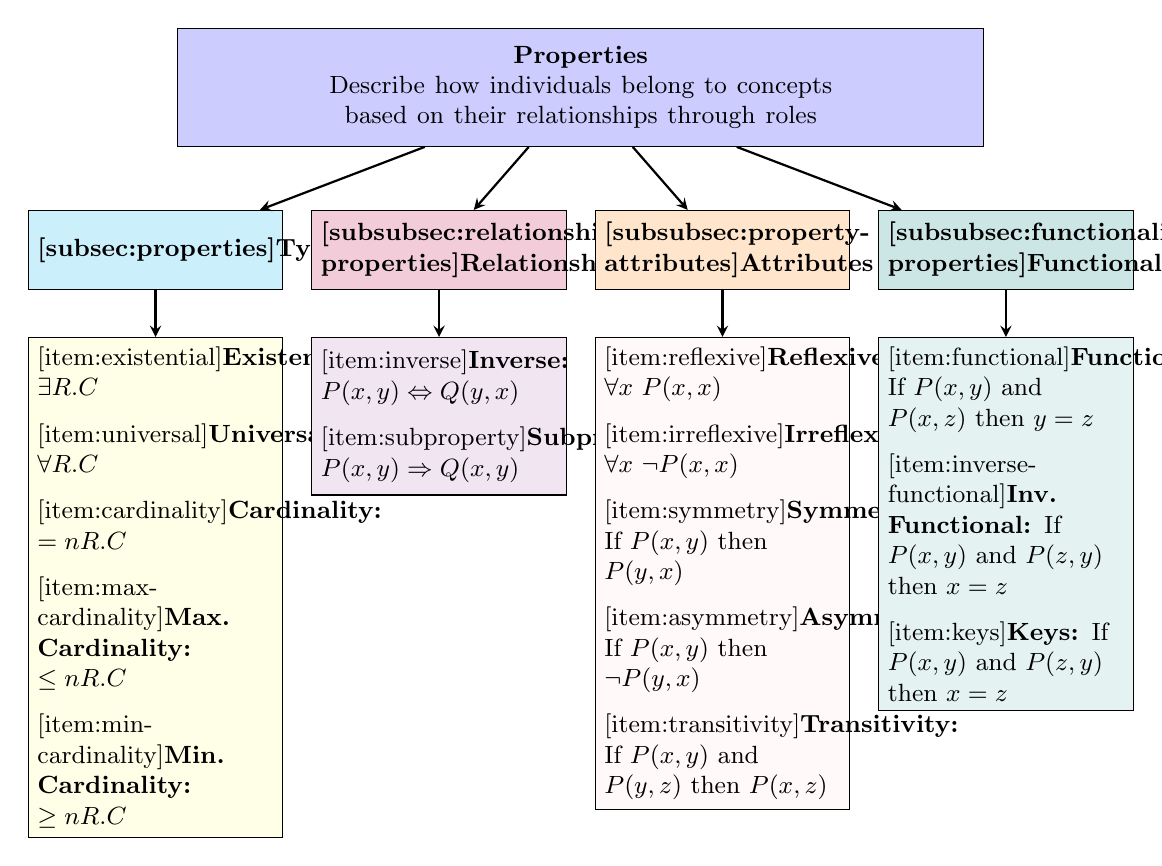
\begin{tikzpicture}[
    node distance=0.8cm and 1.2cm,
    titlebox/.style={rectangle, draw, fill=blue!20, text width=5cm, align=center, minimum height=1cm, font=\small\bfseries},
    defbox/.style={rectangle, draw, fill=green!10, text width=10cm, align=center, minimum height=0.8cm, font=\small},
    typesbox/.style={rectangle, draw, fill=cyan!20, text width=3cm, align=center, minimum height=1cm, font=\small\bfseries},
    typescontent/.style={rectangle, draw, fill=yellow!10, text width=3cm, align=left, minimum height=2.5cm, font=\small},
    attrsbox/.style={rectangle, draw, fill=orange!20, text width=3cm, align=center, minimum height=1cm, font=\small\bfseries},
    attrscontent/.style={rectangle, draw, fill=pink!10, text width=3cm, align=left, minimum height=3cm, font=\small},
    relsbox/.style={rectangle, draw, fill=purple!20, text width=3cm, align=center, minimum height=1cm, font=\small\bfseries},
    relscontent/.style={rectangle, draw, fill=violet!10, text width=3cm, align=left, minimum height=2cm, font=\small},
    funcbox/.style={rectangle, draw, fill=teal!20, text width=3cm, align=center, minimum height=1cm, font=\small\bfseries},
    funccontent/.style={rectangle, draw, fill=teal!10, text width=3cm, align=left, minimum height=2.5cm, font=\small},
    arrow/.style={->, >=stealth, thick}
]

% Main title and definition combined
\node[titlebox, text width=10cm, minimum height=1.5cm] (properties) at (0,0) {\textbf{Properties}\\\normalfont Describe how individuals belong to concepts\\based on their relationships through roles};
\node[typesbox, below=0.8cm of properties, xshift=-5.4cm] (types) {\hyperref[subsec:properties]{Types}};
\node[typescontent, below=0.6cm of types] (types-list) {
    \hyperref[item:existential]{\textbf{Existential:}} $\exists R.C$\\[0.2cm]
    \hyperref[item:universal]{\textbf{Universal:}} $\forall R.C$\\[0.2cm]
    \hyperref[item:cardinality]{\textbf{Cardinality:}} $= n R.C$\\[0.2cm]
    \hyperref[item:max-cardinality]{\textbf{Max. Cardinality:}} $\leq n R.C$\\[0.2cm]
    \hyperref[item:min-cardinality]{\textbf{Min. Cardinality:}} $\geq n R.C$
};
\node[relsbox, below=0.8cm of properties, xshift=-1.8cm] (relationships) {\hyperref[subsubsec:relationships-properties]{Relationships}};
\node[relscontent, below=0.6cm of relationships] (rels-list) {
    \hyperref[item:inverse]{\textbf{Inverse:}} $P(x, y) \Leftrightarrow Q(y, x)$\\[0.2cm]
    \hyperref[item:subproperty]{\textbf{Subproperty:}} $P(x, y) \Rightarrow Q(x, y)$
};
\node[attrsbox, below=0.8cm of properties, xshift=1.8cm] (attributes) {\hyperref[subsubsec:property-attributes]{Attributes}};
\node[attrscontent, below=0.6cm of attributes] (attrs-list) {
    \hyperref[item:reflexive]{\textbf{Reflexive:}} $\forall x \ P(x, x)$\\[0.2cm]
    \hyperref[item:irreflexive]{\textbf{Irreflexive:}} $\forall x \ \neg P(x, x)$\\[0.2cm]
    \hyperref[item:symmetry]{\textbf{Symmetry:}} If $P(x, y)$ then $P(y, x)$\\[0.2cm]
    \hyperref[item:asymmetry]{\textbf{Asymmetry:}} If $P(x, y)$ then $\neg P(y, x)$\\[0.2cm]
    \hyperref[item:transitivity]{\textbf{Transitivity:}} If $P(x, y)$ and $P(y, z)$ then $P(x, z)$
};
\node[funcbox, below=0.8cm of properties, xshift=5.4cm] (functionality) {\hyperref[subsubsec:functionality-properties]{Functionality}};
\node[funccontent, below=0.6cm of functionality] (func-list) {
    \hyperref[item:functional]{\textbf{Functional:}} If $P(x, y)$ and $P(x, z)$ then $y = z$\\[0.2cm]
    \hyperref[item:inverse-functional]{\textbf{Inv. Functional:}} If $P(x, y)$ and $P(z, y)$ then $x = z$\\[0.2cm]
    \hyperref[item:keys]{\textbf{Keys:}} If $P(x, y)$ and $P(z, y)$ then $x = z$
};

\draw[arrow] (properties) -- (types);
\draw[arrow] (types) -- (types-list);
\draw[arrow] (properties) -- (relationships);
\draw[arrow] (relationships) -- (rels-list);
\draw[arrow] (properties) -- (attributes);
\draw[arrow] (attributes) -- (attrs-list);
\draw[arrow] (properties) -- (functionality);
\draw[arrow] (functionality) -- (func-list);

\end{tikzpicture}
}
\caption{Concept map of Properties}
\label{fig:properties-conceptmap}
\end{figure}

\subsection{Reasoning}
\label{subsec:reasoning}

From a knowledge base, reasoning (inference) can be performed. Different types of reasoning tasks allow us to extract information and answer questions about the domain.

\begin{table}[H]
\centering
\caption{Types of Reasoning}
\label{tab:reasoning}
\begin{tabular}{p{5cm}p{9cm}}
\toprule
\textbf{Type of Reasoning} & \textbf{Description} \\
\midrule
\textbf{Concept Satisfaction} & From $\Sigma$ it is not deduced that $C \equiv \bot$ \\
\midrule
\textbf{Subsumption} & $\Sigma \Rightarrow C \sqsubseteq D$ \\
\midrule
\textbf{Instantiation} & $\Sigma \Rightarrow a \in C$ \\
\midrule
\textbf{Information Retrieval} & Given a concept $C$, obtain individuals $a$ such that $a \in C$ \\
\midrule
\textbf{Comprehension} & Given an individual $a$, obtain the most specific concept $C$ such that $a \in C$ \\
\bottomrule
\end{tabular}
\end{table}

\textbf{Explanation of each type}:

\begin{itemize}
    \item \textbf{Concept Satisfaction}: Checks if a given concept $C$ is satisfiable within the knowledge base $\Sigma$, meaning it's not equivalent to the bottom concept ($\bot$), which represents an inconsistent or empty concept. If a concept is unsatisfiable, it means there can be no individuals that belong to it.
    
    \textit{Example}: Check if the concept $Student \sqcap \neg Person$ is satisfiable. If the knowledge base states that all students are persons, then this concept is unsatisfiable (equivalent to $\bot$).
    
    \item \textbf{Subsumption}: Determines if concept $C$ is subsumed by concept $D$ within the knowledge base $\Sigma$, meaning all instances of $C$ are also instances of $D$. This checks if $C$ is a subclass of $D$.
    
    \textit{Example}: Check if $Student \sqsubseteq Person$ holds in the knowledge base. If true, it means every student is also a person.
    
    \item \textbf{Instantiation}: Checks if an individual $a$ is an instance of concept $C$ according to the knowledge base $\Sigma$. This verifies whether a specific individual belongs to a concept.
    
    \textit{Example}: Check if $Student(john)$ holds, i.e., whether John is a student according to the knowledge base.
    
    \item \textbf{Information Retrieval}: Given a concept $C$, retrieves all individuals $a$ such that $a \in C$. This is a query that finds all instances of a concept.
    
    \textit{Example}: Query "find all students" would return all individuals that belong to the $Student$ concept, such as $\{john, alice, bob\}$.
    
    \item \textbf{Comprehension}: Given an individual $a$, finds the most specific concept(s) $C$ such that $a \in C$. This determines what concepts an individual belongs to, focusing on the most specific ones.
    
    \textit{Example}: Given individual $john$, find the most specific concepts he belongs to. If John is a graduate student, the result might be $\{GraduateStudent, Student, Person\}$, but the most specific would be $GraduateStudent$.
\end{itemize}

\subsection{Description Logic ALC - Summary}
\label{subsec:alc-conceptmap}

\begin{figure}[H]
\centering
\resizebox{0.9\textwidth}{!}{
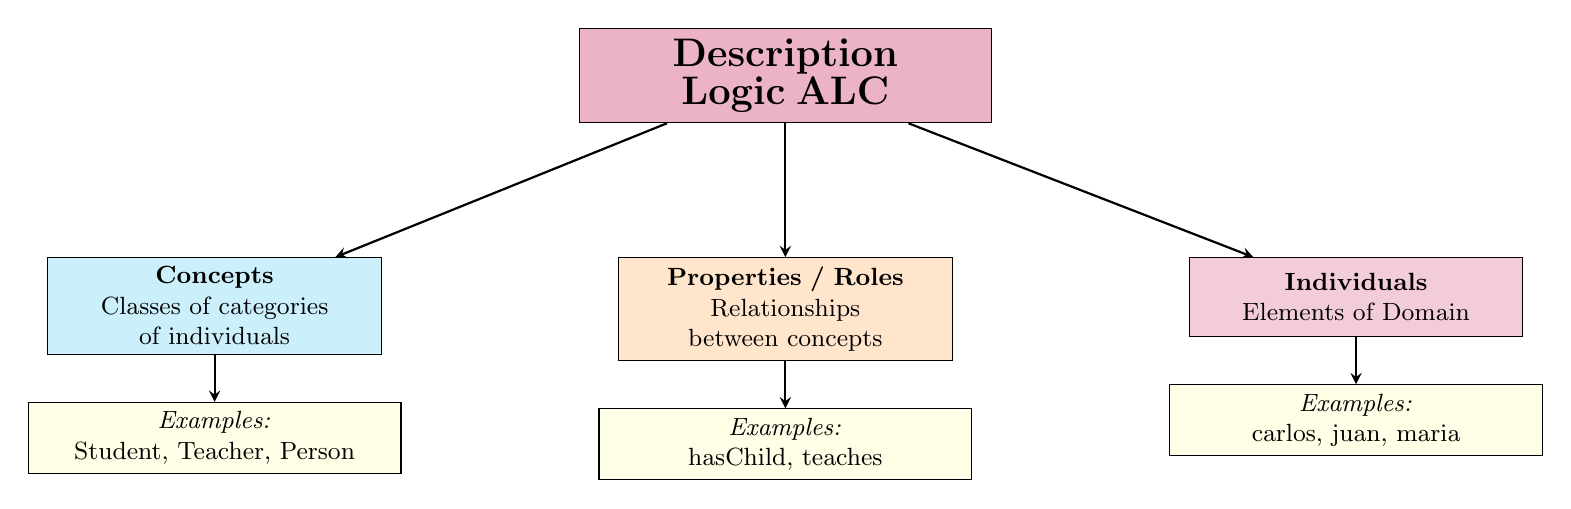
\begin{tikzpicture}[
    node distance=1.2cm and 1.5cm,
    box/.style={rectangle, draw, fill=blue!10, text width=4cm, align=center, minimum height=1cm, font=\small},
    titlebox/.style={rectangle, draw, fill=purple!30, text width=5cm, align=center, minimum height=1.2cm, font=\bfseries},
    defbox/.style={rectangle, draw, fill=green!10, text width=4.5cm, align=center, minimum height=0.8cm, font=\small},
    examplebox/.style={rectangle, draw, fill=yellow!10, text width=4.5cm, align=center, minimum height=0.8cm, font=\small},
    arrow/.style={->, >=stealth, thick}
]

% Main title
\node[titlebox] (main) at (0,0) {\Large Description Logic ALC};

% Left branch: Concepts
\node[box, fill=cyan!20, below left=of main, xshift=-1cm, yshift=-0.5cm] (concepts) {\textbf{Concepts}\\Classes of categories\\of individuals};
\node[examplebox, below=0.6cm of concepts] (concepts-ex) {\textit{Examples:}\\Student, Teacher, Person};

% Middle branch: Properties/Roles
\node[box, fill=orange!20, below=of main, yshift=-0.5cm] (properties) {\textbf{Properties / Roles}\\Relationships\\between concepts};
\node[examplebox, below=0.6cm of properties] (properties-ex) {\textit{Examples:}\\hasChild, teaches};

% Right branch: Individuals
\node[box, fill=purple!20, below right=of main, xshift=1cm, yshift=-0.5cm] (individuals) {\textbf{Individuals}\\Elements of Domain};
\node[examplebox, below=0.6cm of individuals] (individuals-ex) {\textit{Examples:}\\carlos, juan, maria};

% Arrows from main
\draw[arrow] (main) -- (concepts);
\draw[arrow] (main) -- (properties);
\draw[arrow] (main) -- (individuals);

% Arrows to examples
\draw[arrow] (concepts) -- (concepts-ex);
\draw[arrow] (properties) -- (properties-ex);
\draw[arrow] (individuals) -- (individuals-ex);

\end{tikzpicture}
}
\caption{Summary concept map of Description Logic ALC}
\label{fig:alc-summary-conceptmap}
\end{figure}

\section{Higher-Order Logic}
\label{sec:higher-order-logic}

Higher-order logic (or second-order logic) is an extension of first-order logic that adds variables for properties, functions, and relations, along with quantifiers that operate over those variables. This expands the expressive power of the language without having to add new logical symbols.

The need for second-order logic is reflected in Giuseppe Peano's induction axiom for arithmetic, which requires quantifiers that can range not only over concrete elements (like numbers), but also over relations and functions (like properties of numbers).

\textbf{Key distinction}:
\begin{itemize}
    \item \textbf{First-order logic}: Quantifiers only apply to objects. Example: "All students are smart" — $\forall x (Student(x) \rightarrow Smart(x))$
    
    \item \textbf{Higher-order logic}: Quantifiers can also apply to predicates/properties. Example: "All properties that hold for 0 and are preserved by succession hold for all numbers" (mathematical induction).
\end{itemize}

Second-order logic has greater expressive power than first-order logic, allowing the formalization of complex mathematical systems that cannot be captured in first-order logic.

\textbf{Types of Second-Order Logic}:

\begin{itemize}
    \item \textbf{Monadic Second-Order Logic (MSOL)}: Only allows quantification over unary predicates (sets).
    
    \textit{Example}: "There exists a group of people who all speak Spanish" — $\exists Group \forall p (p \in Group \rightarrow SpeaksSpanish(p))$. Here, $Group$ is a variable representing a set of people.
    
    \item \textbf{Full Second-Order Logic (FSOL)}: Allows quantification over predicates of any arity (unary, binary, etc.) and functions.
    
    \textit{Example}: "There exists a relation that is symmetric" — $\exists R \forall x \forall y (R(x,y) \rightarrow R(y,x))$. Here, $R$ is a variable representing a binary relation, like "is friend of".
\end{itemize}

\begin{table}[H]
\centering
\caption{First-Order vs Second-Order Logic}
\label{tab:fol-vs-sol}
\begin{tabular}{p{4.5cm}p{5cm}p{5cm}}
\toprule
\textbf{Aspect} & \textbf{First-Order Logic} & \textbf{Second-Order Logic} \\
\midrule
\textbf{Quantifiers range over} & Objects/individuals & Objects and predicates/relations \\
\midrule
\textbf{Expressive power} & Limited & Greater \\
\midrule
\textbf{Completeness} & Complete & Incomplete \\
\midrule
\textbf{Example} & $\forall x P(x)$ (all objects satisfy $P$) & $\forall P \forall x P(x)$ (all properties hold for all objects) \\
\bottomrule
\end{tabular}
\end{table}

\subsection{Syntax of Second-Order Logic}
\label{subsec:sol-syntax}

Given a vocabulary $\mathcal{L}$, second-order logic (SOL) over $\mathcal{L}$ is defined as an extension of first-order logic that includes the following rules:

\textbf{Formation Rules}:

\begin{itemize}
    \item \textbf{Rule 1}: If $t_1, \ldots, t_k$ are $\mathcal{L}$-terms and $X$ is a second-order variable of arity $k$ (that is, a relation with $k \geq 1$ arguments), then $X(t_1, \ldots, t_k)$ is a formula in SOL.
    
    \textit{Explanation}: We can apply second-order variables (which represent predicates/relations) to first-order terms.
    
    \textit{Example}: If $X$ is a second-order variable of arity 2 (binary relation) and $john$, $mary$ are constants, then $X(john, mary)$ is a valid SOL formula. This could represent "there exists some relation $X$ between John and Mary" (e.g., $X$ could be "knows", "likes", etc.).
    
    \item \textbf{Rule 2}: If $\varphi$ is a formula in SOL and $X$ is a second-order variable of arity $k$, then $\exists X \varphi$ and $\forall X \varphi$ are formulas in SOL.
    
    \textit{Explanation}: We can quantify over second-order variables (predicates/relations).
    
    \textit{Examples}:
    \begin{itemize}
        \item $\exists X \forall x (Student(x) \rightarrow X(x))$ — "There exists a property $X$ that all students have." ($X$ could be "intelligent", "young", etc.)
        
        \item $\forall R \forall x \forall y (R(x,y) \rightarrow R(y,x))$ — "For all binary relations $R$, if $R(x,y)$ holds, then $R(y,x)$ holds." This describes only symmetric relations.
        
        \item $\exists P (P(alice) \land \neg P(bob))$ — "There exists a property $P$ that Alice has but Bob doesn't."
    \end{itemize}
\end{itemize}

\textbf{Note}: The key difference from first-order logic is that in SOL, variables can represent not just objects (like people, numbers), but also predicates and relations (like "is tall", "is greater than", "knows"). This allows us to make statements about properties and relations themselves, not just about individual objects.

\subsection{Semantics of Second-Order Logic}
\label{subsec:sol-semantics}

Given a structure $\mathfrak{A}$ with domain $A$, an assignment $\sigma$ is a function that assigns:

\begin{itemize}
    \item \textbf{A value in $A$ to each first-order variable $x$}: $\sigma(x) \in A$
    
    This is the same as in first-order logic: each variable representing an object gets assigned a concrete object from the domain.
    
    \textit{Example}: If $A = \{john, mary, alice\}$ (set of people), then $\sigma(x) = john$ assigns the person John to variable $x$.
    
    \item \textbf{A subset of $A^k$ to each second-order variable $X$ with $k$ arguments}: $\sigma(X) \subseteq A^k$
    
    Each second-order variable (representing a predicate or relation) gets assigned a set of tuples. For a unary predicate ($k=1$), this is a subset of $A$. For a binary relation ($k=2$), this is a subset of $A \times A$ (pairs of elements).
    
    \textit{Examples}:
    \begin{itemize}
        \item If $P$ is a unary second-order variable (property), then $\sigma(P) = \{john, alice\} \subseteq A$ means that the property $P$ holds for John and Alice, but not for Mary.
        
        For instance, if $P$ represents "speaks Spanish", this assignment says John and Alice speak Spanish, but Mary doesn't.
        
        \item If $R$ is a binary second-order variable (relation with 2 arguments), then $\sigma(R) = \{(john, mary), (alice, john)\} \subseteq A \times A$ means that $R$ relates John to Mary and Alice to John.
        
        For instance, if $R$ represents "knows", this assignment says John knows Mary, and Alice knows John.
    \end{itemize}
\end{itemize}

\textbf{Key insight}: In first-order logic, we only assign concrete objects to variables. In second-order logic, we also assign sets of tuples to second-order variables, which represent the extensions of predicates and relations. This allows us to quantify over all possible predicates and relations, giving SOL its greater expressive power.

\subsection{Additional Semantic Cases for SOL}
\label{subsec:sol-additional-cases}

The definition of SOL includes three additional cases for evaluating formulas with second-order variables:

\textbf{For a second-order variable $X$ with arity $k$}:

\begin{enumerate}
    \item \textbf{Application of second-order variable}:
    \[
    (\mathfrak{A}, \sigma) \models X(t_1, \ldots, t_k) \text{ if and only if } (\sigma(t_1), \ldots, \sigma(t_k)) \in \sigma(X)
    \]
    
    \textit{Meaning}: The formula $X(t_1, \ldots, t_k)$ is satisfied if the tuple of values assigned to the terms $(t_1, \ldots, t_k)$ belongs to the set assigned to the second-order variable $X$.
    
    \textit{Example}: Suppose $X$ is a binary relation, $\sigma(X) = \{(john, mary), (alice, bob)\}$, and $\sigma(t_1) = john$, $\sigma(t_2) = mary$. Then $(\mathfrak{A}, \sigma) \models X(t_1, t_2)$ because $(john, mary) \in \sigma(X)$.
    
    If we think of $X$ as "knows", this says "John knows Mary" is true in this interpretation.
    
    \item \textbf{Existential quantification over second-order variables}:
    \[
    (\mathfrak{A}, \sigma) \models \exists X \varphi \text{ if and only if there exists } S \subseteq A^k \text{ such that } (\mathfrak{A}, \sigma[X/S]) \models \varphi
    \]
    
    \textit{Meaning}: The formula $\exists X \varphi$ is satisfied if there exists some subset $S$ of $A^k$ such that when we assign $S$ to $X$, the formula $\varphi$ becomes true. Here, $\sigma[X/S]$ denotes the assignment that is identical to $\sigma$ except that it assigns $S$ to $X$.
    
    \textit{Example}: Consider $\exists P \forall x (Student(x) \rightarrow P(x))$ — "There exists a property $P$ that all students have."
    
    This is satisfied if we can find some set $S \subseteq A$ (e.g., $S = \{john, mary, alice, bob\}$ representing "all people") such that when we assign $P$ to this set, every student is in that set.
    
    \item \textbf{Universal quantification over second-order variables}:
    \[
    (\mathfrak{A}, \sigma) \models \forall X \varphi \text{ if and only if for every } S \subseteq A^k, (\mathfrak{A}, \sigma[X/S]) \models \varphi
    \]
    
    \textit{Meaning}: The formula $\forall X \varphi$ is satisfied if for every possible subset $S$ of $A^k$, when we assign $S$ to $X$, the formula $\varphi$ is true.
    
    \textit{Example}: Consider $\forall P (P(john) \rightarrow P(mary))$ — "For all properties, if John has the property, then Mary also has it."
    
    This is satisfied if, no matter which property we choose (tall, smart, Spanish-speaking, etc.), whenever John has it, Mary has it too. This would only be true if Mary has all the properties that John has.
\end{enumerate}

\textbf{Summary}: These three cases extend the standard first-order semantics to handle second-order variables. The key difference is that quantifiers in SOL range over sets (subsets of $A^k$), not just individual elements, allowing us to express statements about all possible properties and relations.


\section{Multivalued Logic and Fuzzy Logic}
\label{sec:multivalued-fuzzy-logic}

\subsection{Multivalued Logic}
\label{subsec:multivalued-logic}

Multivalued logic is a logic that allows intermediate values (large, warm, far, few, many, etc.) and uses more than two truth values to describe concepts that go beyond true and false. Multivalued logics provide conceptual tools that make it possible to formally describe fuzzy, vague, or uncertain information.

\textbf{Key characteristics}:
\begin{itemize}
    \item Uses more than two truth values (unlike classical logic which only has true/false)
    \item Allows for degrees of truth (e.g., 0.0 to 1.0, or linguistic values like "very true", "somewhat true", "false")
    \item Suitable for representing imprecise or uncertain information
\end{itemize}

\textbf{Example}: Instead of saying "The temperature is hot" (true/false), multivalued logic allows us to say "The temperature is 0.8 hot" or "The temperature is somewhat hot", representing degrees of truth.

\subsection{Fuzzy Logic}
\label{subsec:fuzzy-logic}

Fuzzy logic (also called fuzzy logic) is a multivalued logic that allows the mathematical representation of uncertainty and vagueness, providing formal tools for their treatment. Lotfi A. Zadeh is considered the father of fuzzy logic. His career focused on work on fuzzy sets and the application of fuzzy logic in approximate reasoning. The term "fuzzy logic" first appeared in 1974.

\begin{tcolorbox}[colback=blue!5!white,colframe=blue!75!black,title=Curious Fact: Zadeh's Principle]
\textbf{Zadeh's Principle} (1973): "As complexity increases, precise statements lose their meaning and useful statements lose precision." 

This can be summarized as "you can't see the forest for the trees" — when dealing with complex systems, trying to be too precise can make statements meaningless, while useful statements often need to sacrifice some precision to remain comprehensible and applicable.
\end{tcolorbox}

\textbf{Key insight}: The model of characterizing a problem through fuzzy logic is based on the prerogative that the mapping between concepts is done through semantics, not numerical precision. It is very suitable for modeling problems from expert knowledge, which normally details their knowledge base in the form of imprecise expressions.

\textbf{Applications in Artificial Intelligence}:
\begin{itemize}
    \item Handling reasoning under uncertainty and with imprecise notions
    \item Management of databases and knowledge-based systems when information is known to be imprecise
    \item Automation of data mining techniques, which are often linked to fuzzy or multivalued sets
    \item Automatic reasoning methods for these logics
\end{itemize}

\subsection{Example: Air Conditioning System}
\label{subsec:fuzzy-ac-example}

Imagine a fuzzy system controlling an air conditioner that regulates temperature according to needs.

\textbf{Inputs}: The fuzzy chips of the air conditioner collect input data, which in this case could be simply:
\begin{itemize}
    \item Temperature
    \item Humidity
\end{itemize}

\textbf{Processing}: These data are subject to the rules of the inference engine (in the form IF... THEN...), which derives a results area.

\textbf{Example rules}:
\begin{itemize}
    \item IF temperature is \textit{very hot} AND humidity is \textit{high}, THEN cooling is \textit{maximum}
    \item IF temperature is \textit{warm} AND humidity is \textit{moderate}, THEN cooling is \textit{moderate}
    \item IF temperature is \textit{cool} AND humidity is \textit{low}, THEN cooling is \textit{minimum}
\end{itemize}

\textbf{Output}: From the results area, the center of gravity is chosen, providing it as an output. According to the result, the air conditioner could increase or decrease the temperature based on the output degree.

\textbf{Key advantage}: Unlike traditional systems that use precise thresholds (e.g., "if temperature > 25°C, turn on"), fuzzy systems handle gradual transitions and imprecise concepts naturally, making them more suitable for human-like reasoning and expert knowledge representation.



\section{Summary - Lecture 003}
\begin{figure}[H]
\centering
\resizebox{1\textwidth}{!}{
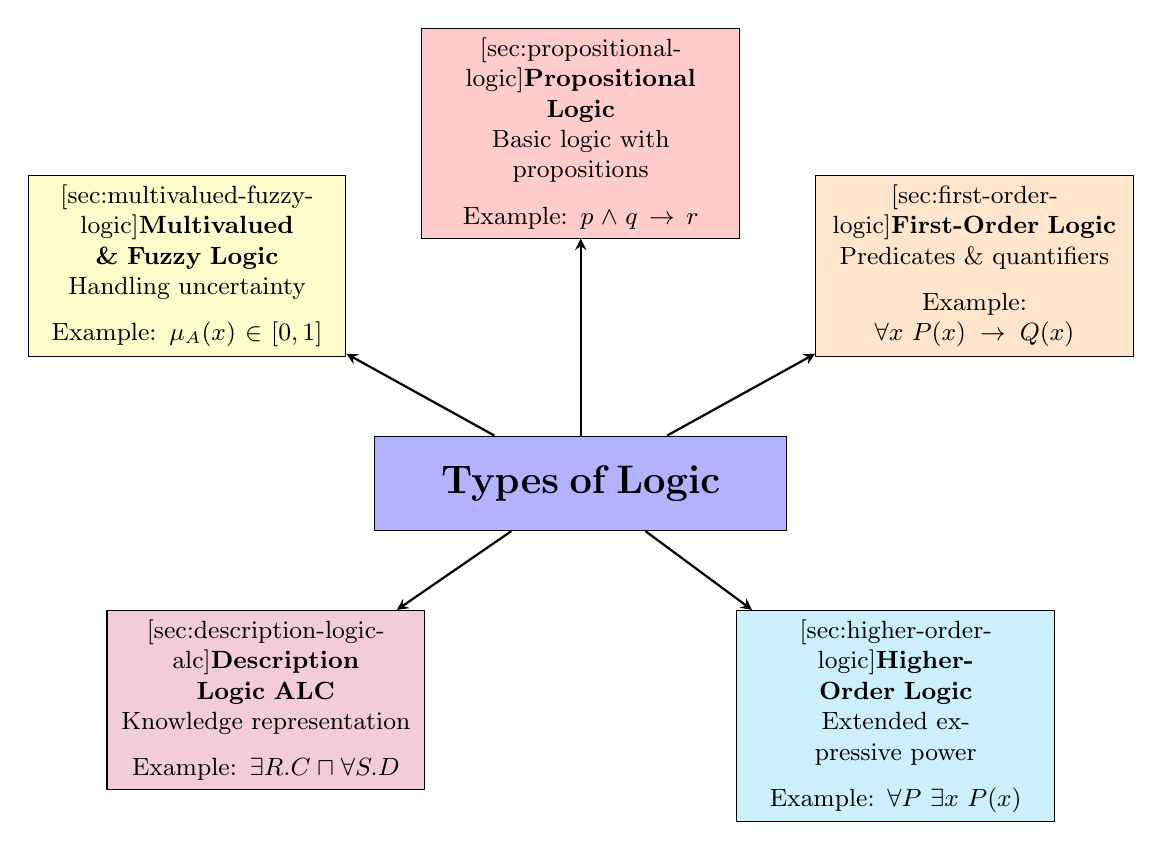
\begin{tikzpicture}[
    node distance=1.3cm and 1.8cm,
    box/.style={rectangle, draw, fill=blue!10, text width=3.8cm, align=center, minimum height=1cm, font=\small},
    titlebox/.style={rectangle, draw, fill=blue!30, text width=5cm, align=center, minimum height=1.2cm, font=\bfseries},
    smallbox/.style={rectangle, draw, fill=green!10, text width=3.2cm, align=left, minimum height=0.8cm, font=\scriptsize},
    arrow/.style={->, >=stealth, thick}
]

% Main title (center)
\node[titlebox] (main) at (0,0) {\Large Types of Logic};

% Positioning around center
\node[box, fill=yellow!20, above=1cm of main, xshift=-5cm] (fuzzy) {\hyperref[sec:multivalued-fuzzy-logic]{\textbf{Multivalued \& Fuzzy Logic}}\\Handling uncertainty\\[0.2cm]Example: $\mu_A(x) \in [0,1]$};

\node[box, fill=red!20, above=2.5cm of main] (prop) {\hyperref[sec:propositional-logic]{\textbf{Propositional Logic}}\\Basic logic with propositions\\[0.2cm]Example: $p \land q \rightarrow r$};

\node[box, fill=orange!20, above=1cm of main, xshift=5cm] (fol) {\hyperref[sec:first-order-logic]{\textbf{First-Order Logic}}\\Predicates \& quantifiers\\[0.2cm]Example: $\forall x \ P(x) \rightarrow Q(x)$};

\node[box, fill=purple!20, below=1cm of main, xshift=-4cm] (alc) {\hyperref[sec:description-logic-alc]{\textbf{Description Logic ALC}}\\Knowledge representation\\[0.2cm]Example: $\exists R.C \sqcap \forall S.D$};

\node[box, fill=cyan!20, below=1cm of main, xshift=4cm] (hol) {\hyperref[sec:higher-order-logic]{\textbf{Higher-Order Logic}}\\Extended expressive power\\[0.2cm]Example: $\forall P \ \exists x \ P(x)$};

% Arrows from main
\draw[arrow] (main) -- (prop);
\draw[arrow] (main) -- (fol);
\draw[arrow] (main) -- (alc);
\draw[arrow] (main) -- (hol);
\draw[arrow] (main) -- (fuzzy);

\end{tikzpicture}
}
\caption{Conceptual map of the Reasoning and Planning course - Lecture 003}
\end{figure}




% Lecture 004
\section*{Lecture 004}
\section{Overview of a Search Problem}
\label{sec:search-problem-overview}

Search problems can be classified according to two main criteria: the use of heuristics and the execution timing. These classifications help us understand the characteristics and behavior of different search algorithms.

\subsection{Uninformed vs. Informed Search}
\label{subsec:uninformed-informed}

The first classification depends on whether the algorithm uses a \textbf{heuristic function} (a function that estimates the cost or distance to the goal):

\begin{itemize}
    \item \textbf{Uninformed search}: Algorithms that do not use any heuristic information. They explore the search space systematically without prior knowledge about which states are more promising. Each state is evaluated equally, without knowing if it brings us closer to the goal.
    
    \item \textbf{Informed search}: Algorithms that employ a heuristic function to guide the search process. The heuristic provides an estimate of how close a state is to the goal, allowing the algorithm to prioritize more promising paths and typically find solutions more efficiently.
\end{itemize}

\subsection{Offline vs. Online Search}
\label{subsec:offline-online}

The second classification relates to when the agent executes actions relative to the search process:

\begin{itemize}
    \item \textbf{Offline search}: The agent first completes the entire search process to find a complete solution plan (from initial state to goal), and only then begins executing the actions. This approach is typical of deliberative agents that have sufficient time to plan before acting.
    
    \item \textbf{Online search}: The agent interleaves search and execution—it searches for a short-term plan, executes some actions, then searches again from the new state. This approach is used by reactive agents operating under time constraints or in dynamic environments. Typically employs local search algorithms that find partial solutions incrementally.
\end{itemize}


\section{Search-Based Agents}
\label{sec:search-based-agents}

\textbf{Search-based agents} are intelligent agents that use search algorithms to find sequences of actions that achieve their goals. These agents operate by maintaining an internal model of their environment and systematically exploring possible action sequences.

\subsection{Key Characteristics}
\label{subsec:search-agents-characteristics}

Search-based agents are characterized by two fundamental properties:

\begin{itemize}
    \item \textbf{Symbolic environment model}: They maintain a symbolic representation of the environment that captures only the information relevant to the problem at hand. This model defines the parameters that distinguish one state from another, allowing the agent to reason about different configurations of the environment.
    
    \item \textbf{Goal-oriented state modification}: They aim to modify the environment state according to their objectives by applying actions that transform the current state into a goal state—one that satisfies the agent's objectives.
\end{itemize}

\subsection{How They Work}
\label{subsec:search-agents-operation}

To achieve their goals, search-based agents follow a systematic approach:

\begin{enumerate}
    \item \textbf{Action anticipation}: Using their environment model, they predict the effects that their actions would have on the world. This allows them to simulate different action sequences without actually executing them.
    
    \item \textbf{Plan generation}: Through a search process, they explore possible sequences of actions that lead from the current state to a goal state. The search algorithm systematically evaluates different paths through the state space.
    
    \item \textbf{Plan execution}: Once a valid sequence is found, the agent executes the plan to transform the environment from its current state to the desired goal state.
\end{enumerate}

The search process is central to these agents—it is the mechanism that allows them to find the appropriate sequence of actions to achieve their objectives.

\subsection{Deliberative vs. Reactive Search-Based Agents}
\label{subsec:deliberative-reactive-search}

The timing of search and execution differs based on the agent type:

\begin{itemize}
    \item \textbf{Deliberative agents}: Complete the entire search process \textit{before} executing any actions. Once a solution plan is found, execution begins. This approach minimizes the risk of costly mistakes.
    
    \item \textbf{Reactive agents}: Interleave search and execution—they search while executing actions. This carries the risk of making mistakes that may require undoing costly actions.
\end{itemize}

\textbf{Note}: Both deliberative and reactive agents can use either \textbf{informed} or \textbf{uninformed} search algorithms.

\section{Domain-Specific Algorithms}
\label{sec:domain-specific-algorithms}

\textbf{Domain-specific algorithms} are problem-solving techniques where the agent designer encodes a known method for solving problems in a particular domain into a specialized algorithm.

\begin{figure}[H]
    \centering
    \includegraphics[width=0.8\textwidth]{img/domainhanoi.png}
    \caption{Example of a domain-specific algorithm: Recursive solution for the Towers of Hanoi problem. This algorithm is specifically designed for this puzzle and cannot be directly applied to other domains.}
    \label{fig:hanoi-algorithm}
\end{figure}

\subsection{How They Work}
\label{subsec:domain-algorithms-operation}

\begin{itemize}
    \item The designer identifies a solution method for a specific problem domain.
    \item This method is encoded into a specialized algorithm that can solve any problem instance within that domain.
    \item Flexibility can be improved by using \textbf{parameters} that configure the problem, allowing the same code to handle different problem instances within the domain.
\end{itemize}

\subsection{Limitations}
\label{subsec:domain-algorithms-limitations}

The main drawbacks of this approach are:

\begin{itemize}
    \item \textbf{Exhaustive anticipation required}: The designer must anticipate all possible scenarios the agent might encounter. In real-world environments, this is often too complex to achieve.
    
    \item \textbf{Domain restriction}: The algorithm only works for the specific domain it was designed for. It cannot be applied to problems outside that domain without significant modification.
\end{itemize}

\section{Domain-Independent Methods}
\label{sec:domain-independent-methods}

\textbf{Domain-independent methods} use a symbolic model of the domain and problem to solve tasks. Unlike domain-specific algorithms, they employ generic search algorithms that work across different problem domains.

\subsection{Problem Representation}
\label{subsec:problem-representation}

For example, in the Towers of Hanoi problem, we would define the problem in general terms as follows:

\begin{figure}[H]
    \centering
    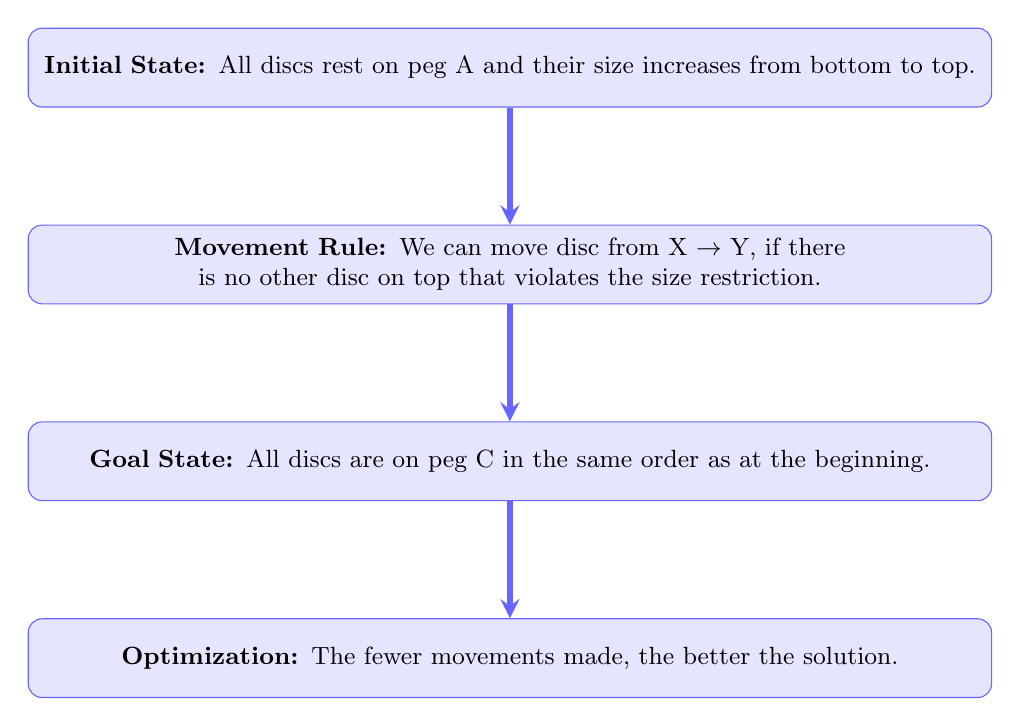
\begin{tikzpicture}[
        box/.style={rectangle, rounded corners=5pt, draw=blue!60, fill=blue!10, text width=12cm, minimum height=1cm, align=center, font=\small},
        arrow/.style={->, >=stealth, blue!60, line width=2pt}
    ]
        % Boxes
        \node[box] (initial) at (0,0) {\textbf{Initial State:} All discs rest on peg A and their size increases from bottom to top.};
        
        \node[box] (rule) at (0,-2.5) {\textbf{Movement Rule:} We can move disc from X $\rightarrow$ Y, if there is no other disc on top that violates the size restriction.};
        
        \node[box] (goal) at (0,-5) {\textbf{Goal State:} All discs are on peg C in the same order as at the beginning.};
        
        \node[box] (optimization) at (0,-7.5) {\textbf{Optimization:} The fewer movements made, the better the solution.};
        
        % Arrows
        \draw[arrow] (initial.south) -- (rule.north);
        \draw[arrow] (rule.south) -- (goal.north);
        \draw[arrow] (goal.south) -- (optimization.north);
    \end{tikzpicture}
    \caption{Symbolic representation of the Towers of Hanoi problem using domain-independent methods.}
    \label{fig:hanoi-problem-definition}
\end{figure}

\subsection{Advantages}
\label{subsec:domain-independent-advantages}

To solve problems, this method employs a \textbf{generic search algorithm}, representing the domain and problem through the symbolic model. This approach offers several advantages:

\begin{itemize}
    \item \textbf{Greater flexibility}: We do not need to know the solution beforehand. The search algorithm explores the solution space automatically.
    
    \item \textbf{Easy extensibility}: It is straightforward to add new features or constraints to the problem by modifying the symbolic model, without changing the search algorithm itself.
    
    \item \textbf{Reusability}: The same generic search algorithm can be applied to different problem domains by simply changing the symbolic representation.
\end{itemize}

\section{State-Space Search Problems}
\label{sec:state-space-search}

In state-space search problems, the environment is represented through \textbf{states} that must be uniquely distinguishable from each other, but lack accessible characteristics that allow direct differentiation. For the agent, they are simply different "labels" representing distinct states.

\subsection{Problem Components}
\label{subsec:problem-components}

This type of problem is defined by three essential elements:

\begin{itemize}
    \item \textbf{State space}: A model of the world represented by a graph, where nodes represent components of the world. These components are translated into elements of the symbolic model, symbolized in a specific way within the graph.
    
    \item \textbf{Search problem}: Through a problem-independent mechanism, we explore the state space by applying the agent's attitude, which represents the rationality component in the exploration process.
    
    \item \textbf{Objective}: To find the most efficient plan that leads from the initial state to a goal state.
\end{itemize}

\subsection{The Search Challenge}
\label{subsec:search-challenge}

Therefore, this type of problem aims to find the best path within a directed graph, as shown in Figure~\ref{fig:state-space-graph}. However, we do not know the graph structure in advance. If we knew it, we could perform a minimum path search using algorithms like Dijkstra's algorithm.

\begin{figure}[H]
    \centering
    \includegraphics[width=0.9\textwidth]{img/graph.png}
    \caption{Example of a state-space search graph. The red nodes and path highlight a possible solution path from the initial state (s1) to a goal state (s12).}
    \label{fig:state-space-graph}
\end{figure}

Since the graph is unknown, we must explore it incrementally through search algorithms, discovering states and transitions as we explore the state space.

\subsection{The Search Process}
\label{subsec:search-process}

The search method operates through an iterative cycle, as illustrated in Figure~\ref{fig:search-method}:

\begin{figure}[H]
    \centering
    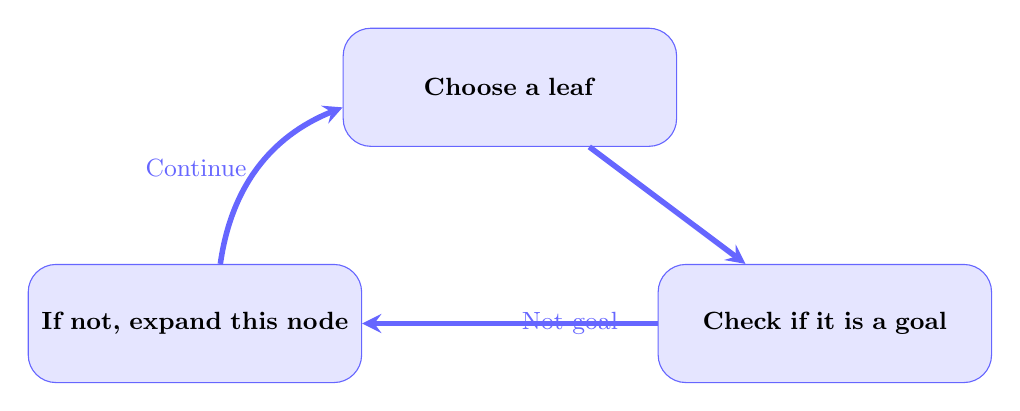
\begin{tikzpicture}[
        box/.style={rectangle, rounded corners=10pt, draw=blue!60, fill=blue!10, text width=4cm, minimum height=1.5cm, align=center, font=\small},
        arrow/.style={->, >=stealth, blue!60, line width=2pt}
    ]
        % Boxes
        \node[box] (choose) at (0,0) {\textbf{Choose a leaf}};
        \node[box] (check) at (4,-3) {\textbf{Check if it is a goal}};
        \node[box] (expand) at (-4,-3) {\textbf{If not, expand this node}};
        
        % Arrows
        \draw[arrow] (choose) -- (check);
        \draw[arrow] (check) -- node[right, font=\small] {Not goal} (expand);
        \draw[arrow, bend left=30] (expand) to node[left, font=\small] {Continue} (choose);
    \end{tikzpicture}
    \caption{Search method based on the selection of a leaf representing a state.}
    \label{fig:search-method}
\end{figure}

The process repeats until a goal state is found. During this exploration, we build a \textbf{search tree} that represents the states we have discovered and explored, as shown in Figure~\ref{fig:search-tree}.

\begin{figure}[H]
    \centering
    \includegraphics[width=0.9\textwidth]{img/tree.png}
    \caption{Example of a search tree showing the exploration of states. Each node represents a state configuration, and edges represent transitions between states.}
    \label{fig:search-tree}
\end{figure}

\begin{figure}[H]
    \centering
    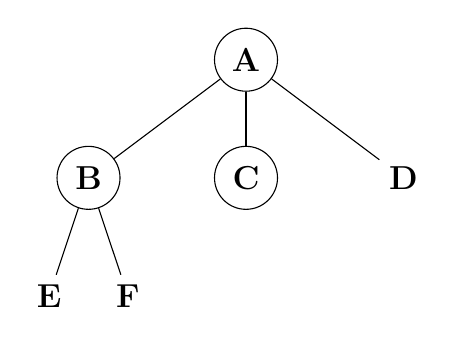
\begin{tikzpicture}[
        node/.style={circle, draw=black, fill=white, minimum size=0.8cm, font=\large\bfseries},
        textnode/.style={font=\large\bfseries}
    ]
        % Tree nodes
        \node[node] (A) at (0,0) {A};
        \node[node] (B) at (-2,-1.5) {B};
        \node[node] (C) at (0,-1.5) {C};
        \node[textnode] (D) at (2,-1.5) {D};
        \node[textnode] (E) at (-2.5,-3) {E};
        \node[textnode] (F) at (-1.5,-3) {F};
        
        % Edges
        \draw (A) -- (B);
        \draw (A) -- (C);
        \draw (A) -- (D);
        \draw (B) -- (E);
        \draw (B) -- (F);
    \end{tikzpicture}
    \caption{Nomenclature for graph traversal in search algorithms. \textbf{Notation:} When expanding, we note the successors from left to right, but the algorithm does not always expand them in that order (another algorithm could have chosen D before, and would then continue on that side of the figure).}
    \label{fig:search-nomenclature}
\end{figure}

\textit{It is a particular way of traversing a graph (it will be different for each algorithm we will see).}

\begin{itemize}
    \item \textbf{A} is a node with initial state (expanded) with three successors B, C, D.
    \item \textbf{B} is a node with state B, expanded, with two successors.
    \item \textbf{C} is a node with state C, expanded, without successors.
    \item \textbf{D} is a node pending expansion (in open list).
    \item \textbf{E} is a node pending expansion (in open list).
    \item \textbf{F} is a node pending expansion (in open list).
\end{itemize}

\subsection{General Search Algorithm}
\label{subsec:general-search-algorithm}

We can define a general search algorithm as shown in the following Python implementation:

\begin{lstlisting}[caption={General search algorithm}, label={lst:general-search}]
def general_search(initial_state, goal_state):
    """
    General search algorithm for state-space problems.
    
    Args:
        initial_state: The starting state S0
        goal_state: The goal state G
    
    Returns:
        Path from initial_state to goal_state, or None if no solution exists
    """
    # Line 1: Initialize open list with initial state
    open_list = [Node(initial_state, parent=None)]
    
    # Line 2: Main search loop
    while open_list:  # While open_list is not empty
        # Line 3: Extract first node from open list
        node = open_list.pop(0)  # FIFO for BFS
        
        # Line 4-5: Check if node is goal
        if is_goal(node.state, goal_state):
            # Return path by backtracking through parent nodes
            return reconstruct_path(node)
        
        # Line 7: Expand node to get successors
        successors = expand(node.state)
        
        # Line 8-10: Add successors to open list
        for successor_state in successors:
            successor_node = Node(successor_state, parent=node)
            open_list.append(successor_node)
    
    # Line 13: No solution found
    return None

class Node:
    """Node representation in the search tree."""
    def __init__(self, state, parent=None):
        self.state = state  # State reached at this point
        self.parent = parent  # Reference to parent node (line 9)
\end{lstlisting}

\subsubsection{Algorithm Components}
\label{subsubsec:algorithm-components}

The search tree is represented using a \textbf{Node} record type. In its simplest form, a node is linked to its predecessor (parent) through a reference (line 112 in the code, where the parent is set in the Node constructor). Each node stores the state reached at that point in the exploration.

\begin{itemize}
    \item \textbf{Open list} (line 85): A list of nodes containing the current leaves of the tree—those states and paths that have been expanded for exploration.
    
    \item \textbf{Empty list check} (line 88): If the list is empty, we have encountered a problem with no solution. Otherwise, we extract the first element from the list of open leaves (line 90).
    
    \item \textbf{Goal check} (lines 93-95): If the node is a goal state, we return the path by performing backtracking through the parent nodes of the found goal node.
    
    \item \textbf{Expansion} (lines 98, 101-103): We expand the node to get successors (line 98), then add the new states obtained from expansion to the open list (lines 101-103).
\end{itemize}

In the following sections, we will show how different uninformed search algorithms work, which are used as the foundation for many intelligent agent problems.

\subsubsection{Repeated States Problem}
\label{subsubsec:repeated-states}

In all search mechanisms, we face a potential problem: \textbf{repeated states}. This can cause serious errors in some cases, such as entering infinite loops. We have different strategies to resolve this:

\begin{itemize}
    \item \textbf{Ignore it}: As strange as it may seem, some algorithms do not have problems with this solution due to their own exploration order.
    
    \item \textbf{Avoid simple cycles}: Prevent adding the parent of a node to the set of successors.
    
    \item \textbf{Avoid general cycles}: Prevent any ancestor of a node from being added to the set of successors.
    
    \item \textbf{Avoid all repeated states}: Do not allow adding any node that already exists in the tree to the set of successors.
\end{itemize}

These strategies must consider the cost of both exploring too much and searching for repeated elements to explore less. The choice depends on the specific problem and the trade-off between memory usage and computational efficiency.

\subsection{Algorithm Classification Criteria}
\label{subsec:algorithm-classification}

In the following sections, we will present different search algorithms. For all of them, we will use a classification mechanism based on the following concepts and characteristics:

\subsubsection{Completeness}
\label{subsubsec:completeness}

An algorithm is \textbf{complete} if it is guaranteed to find a solution whenever one exists. If no solution exists, a complete algorithm will correctly report that no solution was found.

\textit{Example}: Imagine you're searching for your keys in your house. A complete search method would guarantee that if your keys are somewhere in the house, you will eventually find them. If you search room by room systematically, you're using a complete method. However, if you only check the living room and give up, that's an incomplete method—you might miss the keys if they're in the bedroom.

\subsubsection{Optimality}
\label{subsubsec:optimality}

An algorithm is \textbf{optimal} if, when multiple solutions exist, it always finds the best one according to some cost measure (e.g., shortest path, minimum number of steps, lowest cost).

\textit{Example}: Consider finding a route from your home to a restaurant. There might be three routes: Route A (5 km, 10 minutes), Route B (8 km, 8 minutes), and Route C (12 km, 15 minutes). An optimal algorithm would find Route B if you want the fastest route, or Route A if you want the shortest distance. A non-optimal algorithm might find Route C first and stop there, even though better options exist.

\subsubsection{Time Complexity}
\label{subsubsec:time-complexity}

\textbf{Time complexity} measures how long an algorithm takes to find a solution, typically expressed in terms of the problem size (e.g., number of nodes, depth of the search tree).

\textit{Example}: Think of searching for a specific book in a library. If the library has 1,000 books and you check them one by one, you might need to check all 1,000 in the worst case. If the library has 10,000 books, you might need to check all 10,000. The time complexity describes how the search time grows as the library size increases. Some algorithms might need to explore exponentially more states as the problem grows, while others scale more efficiently.

\subsubsection{Space Complexity}
\label{subsubsec:space-complexity}

\textbf{Space complexity} measures how much memory an algorithm requires to find a solution. This includes the storage needed for the open list, closed list, and other data structures.

\textit{Example}: Imagine you're exploring a maze and want to remember all the paths you've tried. A method that stores every path you've explored requires more memory than one that only remembers the current path. If the maze is very large, storing all explored paths might require more memory than your computer has available. Space complexity helps us understand these memory requirements and choose algorithms that fit within available resources.

\section{Breadth-First Search}
\label{sec:breadth-first-search}

\textbf{Breadth-First Search} (BFS) is a search strategy that generates the search tree level by level, expanding all nodes at depth level $i$ before expanding nodes at level $i+1$.

BFS considers, first, all states that are reachable in paths of length 1 (i.e., paths requiring only one action), then those of length 2 (paths requiring two actions), and so on. In this way, it finds the goal state at the minimum depth.

\begin{figure}[H]
    \centering
    \includegraphics[width=0.9\textwidth]{img/bfs_schema.png}
    \caption{Breadth-first search exploration schema. The algorithm explores all nodes at each depth level before moving to the next level.}
    \label{fig:bfs-schema}
\end{figure}

The algorithm develops a search mechanism that, for example, in the 8-puzzle problem, would result in the search tree shown in Figure~\ref{fig:bfs-tree}.

\begin{figure}[H]
    \centering
    \includegraphics[width=0.9\textwidth]{img/bfs_tree.png}
    \caption{Breadth-first search tree for the 8-puzzle problem. The tree is expanded level by level, showing all possible states at each depth.}
    \label{fig:bfs-tree}
\end{figure}

\subsection{Algorithm Implementation}
\label{subsec:bfs-implementation}

The breadth-first search algorithm can be derived from the general search algorithm previously presented, with the following modifications:

\begin{itemize}
    \item \textbf{Adding successors}: New successors are added to the \textit{end} of the open list.
    
    \item \textbf{Queue behavior}: The open list functions as a queue (inserting at the end and retrieving from the beginning), which ensures that the oldest nodes (i.e., those at the shallowest depth) are always expanded first.
    
    \item \textbf{Visited nodes control}: Additionally, we control nodes that have been visited previously to avoid revisiting states.
\end{itemize}

\subsection{Properties}
\label{subsec:bfs-properties}

This algorithm is \textbf{complete} and \textbf{optimal} (finds the shortest path when all actions have the same cost), but it presents very poor time and space complexity, as it depends proportionally on the depth level $d$ of the solution and, therefore, on the number of expanded nodes or branching factor $b$.

\begin{figure}[H]
    \centering
    \includegraphics[width=0.9\textwidth]{img/bfs_complexity.png}
    \caption{Time complexity analysis for breadth-first search in worst case, average case, and best case scenarios. The complexity is $O(b^d)$ where $b$ is the branching factor and $d$ is the depth of the solution.}
    \label{fig:bfs-complexity}
\end{figure}

As shown in Figure~\ref{fig:bfs-complexity}, the time complexity is $O(b^d)$ in all cases:
\begin{itemize}
    \item \textbf{Worst case}: Explores all nodes up to depth $d$: $1 + b + \ldots + b^{d-1} + b^d \in O(b^d)$
    \item \textbf{Average case}: Explores approximately half of the nodes at depth $d$: $1 + b + \ldots + b^{d-1} + b^d/2 \in O(b^d)$
    \item \textbf{Best case}: Finds the goal as the first node at depth $d$: $1 + b + \ldots + b^{d-1} + 1 \in O(b^d)$
\end{itemize}

The space complexity is also $O(b^d)$ because the algorithm must store all nodes at the deepest level in the open list.

\subsection{Example}
\label{subsec:bfs-example}

Let us illustrate BFS with a concrete example. Consider the weighted graph shown in Figure~\ref{fig:search-example}, where we want to find a path from the initial state $S$ to one of the goal states ($G1$ or $G2$).

\begin{figure}[H]
    \centering
    \includegraphics[width=0.9\textwidth]{img/search_example.png}
    \caption{Example search problem: finding a path from initial state $S$ to goal states $G1$ or $G2$. Edge weights represent the cost of transitions. \textbf{Note:} In this BFS example, all edge costs are treated as 1 (uniform cost), so the algorithm finds the shortest path in terms of number of steps, not total cost.}
    \label{fig:search-example}
\end{figure}

Table~\ref{tab:bfs-expansion} shows the step-by-step execution of BFS on this problem. The algorithm expands nodes level by level, and we can see how repeated states are avoided.

\begin{table}[H]
    \centering
    \begin{tabular}{|p{3cm}|p{4cm}|>{\raggedright\arraybackslash}p{7.5cm}|}
        \hline
        \textbf{Expanded} & \textbf{Generates} & \textbf{Open} \\
        \hline
        $S$ & $B, C$ & $B (SB), C (SC)$ \\
        \hline
        $B (SB)$ & $A, E$ & $C (SC), A (SBA), E (SBE)$ \\
        \hline
        $C (SC)$ & $D, G1, \cancel{B}$ & $A (SBA), E (SBE), D (SCD), G1 (SCG1)$ \\
        \hline
        $A (SBA)$ & $\cancel{C}$ & $E (SBE), D (SCD), G1 (SCG1)$ \\
        \hline
        $E (SBE)$ & $F, \cancel{D}$ & $D (SCD), G1 (SCG1), F (SBEF)$ \\
        \hline
        $D (SCD)$ & $G2, \cancel{F}$ & $G1 (SCG1), F (SBEF), G2 (SCDG2)$ \\
        \hline
        $G1 (SCG1)$ & \textbf{FIN} & --- \\
        \hline
    \end{tabular}
    \caption{BFS expansion process for the example problem. The path notation (e.g., $SB$) indicates the path from $S$ to the node. Nodes with strikethrough ($\cancel{X}$) represent states that would be generated but are skipped because they have already been visited or are in the open list, preventing cycles and redundant exploration. \textbf{Note:} Generated nodes are listed in alphabetical order for convention. All edge costs are treated as 1 in this BFS example.}
    \label{tab:bfs-expansion}
\end{table}

\textbf{Solution summary:}
\begin{itemize}
    \item \textbf{Solution:} $SC, CG1$
    \item \textbf{Length:} 2
    \item \textbf{Expanded:} 6 nodes
    \item \textbf{Generated:} 8 nodes (excluding repeated states)
    \item \textbf{Iterations:} 7
\end{itemize}

In this example, BFS finds the goal $G1$ through the path $S \rightarrow C \rightarrow G1$ (2 steps). Notice how the algorithm systematically explores all nodes at depth 1 ($B, C$) before moving to depth 2 ($A, E, D, G1$), and how it avoids generating states that have already been visited.

\section{Depth-First Search}
\label{sec:depth-first-search}

\textbf{Depth-First Search} (DFS) is another uninformed search strategy (without additional information). Unlike breadth-first search, DFS attempts to develop a path of indeterminate length, trying to reach deep goals (those that have a long path to reach them) by developing the fewest possible branches.

In general, DFS works well when combined with additional information, but it can solve problems in the same way as a breadth-first algorithm.

\begin{figure}[H]
    \centering
    \includegraphics[width=0.9\textwidth]{img/dfs_tree.png}
    \caption{Example of how the search tree is generated with the depth-first search algorithm. The red path highlights the exploration sequence, showing how DFS goes deep before backtracking.}
    \label{fig:dfs-tree}
\end{figure}

In this strategy, the tree is expanded from ``left to right,'' so the deepest nodes are expanded first. If a node without successors is reached, the algorithm backtracks and expands the next deepest node.

As a result, the method explores a ``current path'' and does not always find the node at minimum depth. The general algorithm is adapted with the following considerations:

\begin{itemize}
    \item \textbf{Adding successors}: New successors are added to the \textit{beginning} of the open list.
    
    \item \textbf{Stack behavior}: The open list functions as a stack (inserting at the beginning and extracting from the beginning), so we always extract the deepest node. By storing all successors of an expanded node in the open list, we allow ``backtracking.''
    
    \item \textbf{Visited nodes control}: We only process a node from the stack if it has not been visited yet.
\end{itemize}

\subsection{Properties}
\label{subsec:dfs-properties}

The analysis of this algorithm shows that it is \textbf{complete} (if and only if we guarantee the elimination of repeated states within the same branch), but it is \textbf{not optimal} (for cost-one operators), since it does not guarantee that it will always find the solution at the minimum depth.

DFS has the following characteristics:
\begin{itemize}
    \item \textbf{Completeness}: Complete only if repeated states within the same branch are eliminated. Without this control, DFS can get stuck in infinite loops in graphs with cycles.
    
    \item \textbf{Optimality}: Not optimal—it may find a solution, but not necessarily the shortest one, as it explores deep paths first rather than systematically exploring by depth level.
    
    \item \textbf{Time complexity}: $O(b^m)$ in the worst case, where $b$ is the branching factor and $m$ is the maximum depth of the search tree. This can be much worse than BFS if the solution is shallow.
    
    \item \textbf{Space complexity}: $O(bm)$—much better than BFS, as it only needs to store the current path from root to leaf, not all nodes at a given depth level.
\end{itemize}

\subsection{Example}
\label{subsec:dfs-example}

Let us illustrate DFS with the same example graph used for BFS. Consider the weighted graph shown in Figure~\ref{fig:dfs-search-example}, where we want to find a path from the initial state $S$ to one of the goal states ($G1$ or $G2$).

\begin{figure}[H]
    \centering
    \includegraphics[width=0.9\textwidth]{img/search_example.png}
    \caption{Example search problem: finding a path from initial state $S$ to goal states $G1$ or $G2$. Edge weights represent the cost of transitions. \textbf{Note:} In this DFS example, all edge costs are treated as 1 (uniform cost), and nodes are generated in inverse alphabetical order for convention.}
    \label{fig:dfs-search-example}
\end{figure}

Table~\ref{tab:dfs-expansion} shows the step-by-step execution of DFS on this problem. Notice how DFS explores deep paths first, going as far as possible before backtracking.

\begin{table}[H]
    \centering
    \begin{tabular}{|p{3cm}|p{4cm}|>{\raggedright\arraybackslash}p{7.5cm}|}
        \hline
        \textbf{Expanded} & \textbf{Generates} & \textbf{Open} \\
        \hline
        $S$ & $C, B$ & $B (SB), C (SC)$ \\
        \hline
        $B (SB)$ & $E, A$ & $A (SBA), E (SBE), C (SC)$ \\
        \hline
        $A (SBA)$ & $\cancel{C}$ & $E (SBE), C (SC)$ \\
        \hline
        $E (SBE)$ & $F, D$ & $D (SBED), F (SBEF), C (SC)$ \\
        \hline
        $D (SBED)$ & $G2, \cancel{F}$ & $G2 (SBEDG2), F (SBEF), C (SC)$ \\
        \hline
        $G2 (SBEDG2)$ & \textbf{FIN} & --- \\
        \hline
    \end{tabular}
    \caption{DFS expansion process for the example problem. The path notation (e.g., $SB$) indicates the path from $S$ to the node. Nodes with strikethrough ($\cancel{X}$) represent states that would be generated but are skipped because they have already been visited or are in the open list, preventing cycles and redundant exploration. \textbf{Note:} Generated nodes are listed in inverse alphabetical order for convention. All edge costs are treated as 1 in this DFS example.}
    \label{tab:dfs-expansion}
\end{table}

\textbf{Solution summary:}
\begin{itemize}
    \item \textbf{Solution:} $SB, BE, ED, DG2$
    \item \textbf{Length:} 4
    \item \textbf{Expanded:} 5 nodes
    \item \textbf{Generated:} 7 nodes (excluding repeated states)
    \item \textbf{Iterations:} 6
\end{itemize}

In this example, DFS finds the goal $G2$ through the path $S \rightarrow B \rightarrow E \rightarrow D \rightarrow G2$ (4 steps). Notice how DFS explores deep into the tree (following the path $S \rightarrow B \rightarrow E \rightarrow D$) before finding the goal, unlike BFS which would have found a shorter path. This demonstrates that DFS is not optimal—it finds a solution, but not necessarily the shortest one.

\section{Uniform Cost Search}
\label{sec:uniform-cost-search}

In the previous cases of breadth-first and depth-first search, we assumed that the cost of applying any action (and therefore, the cost of choosing a branch) was always equal to 1, so the total cost of a path was the number of levels at which a particular node was located. But what happens when the cost of transitioning from one node to another is not equal for all actions in the environment?

To solve this type of scenario where the cost is not equal for all actions (but is positive in all cases), we have the \textbf{Uniform Cost Search} (UCS) algorithm.

\subsection{Algorithm Overview}
\label{subsec:ucs-overview}

Using the same general search algorithm, we apply the idea of directing the search by the cost of the operators. We assume there exists a utility function $f(n) = g(n)$ that allows us to calculate the real cost to reach node $n$ from the initial node. In each iteration of the algorithm, we will expand first the node with the lowest cost $f$.

For simplicity, in the rest of the explanation of this algorithm, we will refer to the utility function interchangeably as $f$ or $g$.

\subsection{Algorithm Modifications}
\label{subsec:ucs-modifications}

The modifications made to the general search algorithm are:

\begin{itemize}
    \item \textbf{Priority-based storage}: We store each node by priority based on its $g$ value. Therefore, the insertion of new nodes in the open list will be ordered in ascending order according to their $g$ value.
    
    \item \textbf{Priority queue}: The above makes the open list a priority queue ordered by the $g$ value.
    
    \item \textbf{Duplicate prevention}: We only add a node to the open list if it is not already in it.
    
    \item \textbf{Cost update}: If a node is found in the open list, we replace it if and only if the new cost $f$ is lower.
\end{itemize}

\subsection{Properties}
\label{subsec:ucs-properties}

This algorithm is \textbf{complete} and \textbf{optimal} when all costs have positive integer values. Therefore, the sequence of $g$ values is unbounded, and we always expand according to the insertion order based on this same function.

UCS has the following characteristics:
\begin{itemize}
    \item \textbf{Completeness}: Complete when all edge costs are positive. If costs can be zero, completeness is guaranteed only if we ensure no infinite paths with zero cost exist.
    
    \item \textbf{Optimality}: Optimal—always finds the path with the lowest total cost from the initial state to the goal, as it expands nodes in order of increasing path cost.
    
    \item \textbf{Time complexity}: $O(b^{1+\lfloor C^*/\epsilon \rfloor})$, where $C^*$ is the cost of the optimal solution and $\epsilon$ is the minimum edge cost. In practice, this can be exponential.
    
    \item \textbf{Space complexity}: $O(b^{1+\lfloor C^*/\epsilon \rfloor})$—same as time complexity, as all nodes with cost less than the optimal solution cost may be stored.
\end{itemize}

UCS can be seen as a generalization of BFS: when all edge costs are equal to 1, UCS behaves exactly like BFS.

\subsection{Example}
\label{subsec:ucs-example}

Let us illustrate UCS with the same example graph. Consider the weighted graph shown in Figure~\ref{fig:ucs-search-example}, where we want to find the lowest-cost path from the initial state $S$ to one of the goal states ($G1$ or $G2$). Unlike BFS and DFS, UCS considers the actual edge costs.

\begin{figure}[H]
    \centering
    \includegraphics[width=0.9\textwidth]{img/search_example.png}
    \caption{Example search problem: finding the lowest-cost path from initial state $S$ to goal states $G1$ or $G2$. Edge weights represent the actual costs of transitions. \textbf{Note:} In UCS, nodes are generated in alphabetical order, and this order is also used for tie-breaking in the open list when $g$ values are equal.}
    \label{fig:ucs-search-example}
\end{figure}

Table~\ref{tab:ucs-expansion} shows the step-by-step execution of UCS on this problem. Notice how UCS expands nodes in order of increasing path cost $g$, and updates nodes in the open list when better paths are found.

\begin{table}[H]
    \centering
    \begin{tabular}{|p{2.5cm}|p{3.5cm}|>{\raggedright\arraybackslash}p{4.5cm}|>{\raggedright\arraybackslash}p{4.5cm}|}
        \hline
        \textbf{Expanded} & \textbf{Generates} & \textbf{Open} & \textbf{Closed} \\
        \hline
        $S$ & $B (g=1), C (g=4)$ & $B (g=1), C (g=4)$ & $S$ \\
        \hline
        $B (g=1)$ & $A (g=2), E (g=8)$ & $A (g=2), C (g=4), E (g=8)$ & $S, B (g=1)$ \\
        \hline
        $A (g=2)$ & $C (g=3)$ & $C (g=3), \cancel{C (g=4)}, E (g=8)$ & $S, B (g=1), A (g=2)$ \\
        \hline
        $C (g=3)$ & $D (g=8), G1 (g=24)$ ($B$ repeated in path to $C$) & $D (g=8), E (g=8), G1 (g=24)$ & $S, B (g=1), A (g=2), C (g=3)$ \\
        \hline
        $D (g=8)$ & $F (g=14), G2 (g=19)$ & $E (g=8), F (g=14), G2 (g=19), G1 (g=24)$ & $S, B (g=1), A (g=2), C (g=3), D (g=8)$ \\
        \hline
        $E (g=8)$ & $D (g=11), F (g=18)$ ($D$ and $F$ worse than existing paths) & $F (g=14), G2 (g=19), G1 (g=24)$ & $S, B (g=1), A (g=2), C (g=3), D (g=8), E (g=8)$ \\
        \hline
        $F (g=14)$ & (no successors) & $G2 (g=19), G1 (g=24)$ & $S, B (g=1), A (g=2), C (g=3), D (g=8), E (g=8), F (g=14)$ \\
        \hline
        $G2 (g=19)$ & \textbf{FIN} & --- & $S, B (g=1), A (g=2), C (g=3), D (g=8), E (g=8), F (g=14)$ \\
        \hline
    \end{tabular}
    \caption{UCS expansion process for the example problem. The path notation shows the path from $S$ to the node, and $g$ values represent the total cost. Nodes with strikethrough ($\cancel{X}$) represent states that are replaced when a better path is found. The closed list tracks all expanded nodes. \textbf{Note:} Generated nodes are listed in alphabetical order, and this order is used for tie-breaking when $g$ values are equal.}
    \label{tab:ucs-expansion}
\end{table}

\textbf{Solution summary:}
\begin{itemize}
    \item \textbf{Solution:} $SB(1), BA(1), AC(1), CD(5), DG2(11)$
    \item \textbf{Cost:} $1 + 1 + 1 + 5 + 11 = 19$
    \item \textbf{Expanded:} 7 nodes
    \item \textbf{Generated:} 11 nodes (some were never inserted into the open list due to worse costs)
\end{itemize}

In this example, UCS finds the goal $G2$ through the path $S \rightarrow B \rightarrow A \rightarrow C \rightarrow D \rightarrow G2$ with total cost 19. Notice how UCS:
\begin{itemize}
    \item Expands nodes in order of increasing cost (first $B$ with $g=1$, then $A$ with $g=2$, then $C$ with $g=3$, etc.)
    \item Updates node $C$ when a better path is found (replacing $C(g=4)$ with $C(g=3)$)
    \item Ignores worse paths (e.g., $D(g=11)$ and $F(g=18)$ from $E$ are not added because better paths already exist)
    \item Finds the optimal solution with the lowest total cost, unlike DFS which found a longer path
\end{itemize}


\newpage
\bibliographystyle{plainnat}
\bibliography{References}

\end{document}
